
After preselection, a final selection is required to optimize signal-to-background efficiency. A boosted decision tree (BDT) is trained and tested on signal and background MC, with one BDT per signal hypothesis, and a final cut is applied to each BDT discriminator. 

Training samples are constructed by randomly selecting events from the combined 2016, 2017, and 2018 MC datasets detailed in Section~\ref{sec:Samples}. The same background normalization scale factors, data and MC corrections, b-jet requirement, and preselection described in Sections~\ref{sec:EventSelection} and~\ref{sec:Corrections} are applied to the corresponding year's MC. Additional cuts of $\Muu > \SI{250}{\GeV}$ and $\Muujj > \MLQ$ are applied, to reduce training bias in background-enriched and low-signal regions. After training, a separate sample is constructed from the same MC and in the same way, and tested on each BDT to verify there is no overfitting (there is no overlap in training and testing events). A set of 11 kinematic variables---identified for their strong signal-to-background separation power---are used as input variables to the BDTs: 
\begin{itemize}
    \item Invariant masses: \Muu, \Muujj, \MujOne, \MujTwo
    \item Final state object momenta: \ptof{\PmuOne}, \ptof{\PmuTwo}, \ptof{\PjOne}, \ptof{\PjTwo}
    \item Combined momenta: \ST, \MET
    \item Spatial separation between the dimuon pair and the leading-\pt jet: \DRof{\PmuOne+\PmuTwo}{\PjOne}
\end{itemize}
Further details, including a number of studies, can be found in Appendix~\ref{app:BDTPerformance}.

To extract the highest possible signal, a cut on the BDT response is optimized using the Punzi significance~\cite{Punzi} as a figure of merit, defined here:

\begin{equation}
    \frac{\epsilon(t)}{a/2+\sqrt{B(t)}}
    \label{eq:punzi}
\end{equation}

where $\epsilon(t)$ is the signal efficiency for a cut $t$, $a$ is the chosen sigma significance ($a = 5$ in this analysis), and $B(t)$ is the number of background events after applying a cut $t$.

A comparison between observed and expected data at preselection in the BDT score at every leptoquark mass point is shown in Figures~\ref{figapp:BDT300to1400}--\ref{figapp:BDT2700to4000}. Final selection cuts are optimized and applied to the BDT score for each leptoquark mass, while the same cut value is used accross all years. A cut log is listed in Table~\ref{tab:cutlog}. To ensure all events at final selection are contained within the signal region (SR) and do not overlap with events in the background normalization CRs (where the SR and CRs are defined in Table~\ref{tab:srcrdefs}), an additional cut of $\Muu > \SI{250}{\GeV}$ is applied. Additionally, the same \MLQ-dependent cut used in the BDT training is applied at final selection: $\Muujj > \MLQ$. Efficiency in signal and background from applying each final selection cut is shown in Fig.~\ref{figapp:efficiency} for all three years of data-taking. Efficiency here is defined as the number of events passing the final selection (optimized BDT score, $\Muu > \SI{250}{\GeV}$, and $\Muujj > \MLQ$ cuts) divided by the number of events present at preselection (in both the numerator and denominator, the b-jet tag requirement, normalization scale factors, and MC corrections are applied). Event yields at final selection are provided for each year of data taking in Tables~\ref{tab:eventyields2016}--\ref{tab:eventyields2018}. W+Jets has been ommited from the tables as no events pass the final selection---it is kept in the analysis for the background normalization estimation, BDT training, systematic uncertainty estimation, etc. Figures~\ref{figapp:finalSelMuu}--\ref{figapp:finalSelDRuuj1} show the BDT input variables at final selection in 2016, 2017, and 2018 signal and background simulation for several representative leptoquark mass points. Plots showing the Punzi significance as a function of the BDT score, for each BDT, are shown in Figs.~\ref{figapp:punzivsbdt1}--\ref{figapp:punzivsbdt2}.

\begin{table}[H]
    \caption{The \ZJETS (A), \ttbar (B), and $\VV + \TTV$ (C) background normalization CR, and SR definitions.}
    \begin{center}
           %\scriptsize
           \begin{tabular}{cccc}\hline\hline
                Region      & Mass window [\GeV]                 & Additional selection \\ \hline
                Control A   & $80 < \Muu < 100$     & $N_{\jets} = 2$, $N_{\jets} = 3$, $N_{\jets} = 4$, or $N_{\jets} \geq 5$ \\ 
                Control B   & $100 < \Muu < 250$    & - \\ 
                Control C   & $80 < \Muu < 100$     & $N_{\text{leptons}}\geq 3$, $N_{\text{b-jets}}\geq 0$ \\
                Signal      & $250 < \Muu$          & - \\ \hline\hline
           \end{tabular}
           \label{tab:srcrdefs}
    \end{center}
\end{table}


%%%%%%%%%%%%%%%%%%%%%%%%%%%%%%%%%%%%%%%%%%%%%%%%%%%%%%%%%%%%%%%%%%%%%%%%%%%%%%%%%%%%%%%%%%
%%%%%%%%%%%%%%%%%%%%%%%%%%%%%%%%%%%%%%%%%% 2016 %%%%%%%%%%%%%%%%%%%%%%%%%%%%%%%%%%%%%%%%%%
%%%%%%%%%%%%%%%%%%%%%%%%%%%%%%%%%%%%%%%%%%%%%%%%%%%%%%%%%%%%%%%%%%%%%%%%%%%%%%%%%%%%%%%%%%




% 2016 final sel + pt20 veto

\begin{table}[H]
	\tiny
	\begin{center}
		\caption{Event yields in 2016 data at the final selection level. Uncertainties are statistical unless otherwise indicated.}
		\begin{tabular}{ccccccccc}
			\hline \hline
            \MLQ  &     Signal &              	 \ZJETS &                       \ttbar &                    \TTV &           	    \VV &                       Single Top &            All BG (stat + syst)&                               Data \\ \hline	
            300  &      18810 $\pm$ 240  &    	 0.686 $\pm$ 0.089  &           0.13 $\pm$ 0.13  &          0.0423 $\pm$ 0.0061  &  0.242 $\pm$ 0.059  &        0.0 $\pm$ 0.0  &        1.1 $\pm$ 0.16  $\pm$ 0.11  &                       0 \\
            400  &      5501 $\pm$ 59  &      	 0.79 $\pm$ 0.11  &             0.0 $ _{-0.0}^{+0.13}$   &  0.012 $\pm$ 0.003  &    0.0 $ _{-0.0}^{+0.014}$   & 0.378 $\pm$ 0.267  &    1.18 $ _{-0.29}^{+0.32}$   $\pm$ 0.13  &            0 \\
            500  &      3405 $\pm$ 24  &      	 0.719 $\pm$ 0.078  &           0.586 $\pm$ 0.338  &        0.025 $\pm$ 0.005  &    0.0537 $\pm$ 0.019  &       0.407 $\pm$ 0.288  &    1.79 $\pm$ 0.45  $\pm$ 0.12  &                      2 \\
            600  &      1379.9 $\pm$ 8.9  &   	 0.218 $\pm$ 0.031  &           0.0 $ _{-0.0}^{+0.13}$   &  0.018 $\pm$ 0.005  &    0.0462 $\pm$ 0.0207  &      0.0 $\pm$ 0.0  &        0.282 $ _{-0.037}^{+0.131}$   $\pm$ 0.037  &        0 \\
            700  &      706.9 $\pm$ 4.0  &    	 0.283 $\pm$ 0.035  &           0.0 $ _{-0.0}^{+0.13}$   &  0.021 $\pm$ 0.004  &    0.0 $ _{-0.0}^{+0.014}$   & 0.0 $\pm$ 0.0  &        0.304 $ _{-0.035}^{+0.132}$   $\pm$ 0.053  &        0 \\
            800  &      333.1 $\pm$ 1.7  &    	 0.0 $ _{-0.0}^{+0.011}$   &    0.0 $ _{-0.0}^{+0.13}$   &  0.0057 $\pm$ 0.0015  &  0.0063 $\pm$ 0.0032  &      0.0 $\pm$ 0.0  &        0.012 $ _{-0.003}^{+0.127}$   $\pm$ 0.001  &        0 \\
            900  &      165.48 $\pm$ 0.81  &  	 0.103 $\pm$ 0.013  &           0.0 $ _{-0.0}^{+0.13}$   &  0.011 $\pm$ 0.004  &    0.065 $\pm$ 0.026  &        0.0 $\pm$ 0.0  &        0.179 $ _{-0.03}^{+0.129}$   $\pm$ 0.018  &         0 \\
            1000  &     83.44 $\pm$ 0.46  &   	 0.15 $\pm$ 0.018  &            0.0 $ _{-0.0}^{+0.13}$   &  0.01 $\pm$ 0.004  &     0.058 $\pm$ 0.026  &        0.0 $\pm$ 0.0  &        0.219 $ _{-0.032}^{+0.13}$   $\pm$ 0.024  &         1 \\
            1100  &     45.57 $\pm$ 0.2  &    	 0.4 $\pm$ 0.047  &             0.0 $ _{-0.0}^{+0.13}$   &  0.0181 $\pm$ 0.0064  &  0.0415 $\pm$ 0.0207  &      0.0 $\pm$ 0.0  &        0.46 $ _{-0.052}^{+0.136}$   $\pm$ 0.086  &         1 \\
            1200  &     21.345 $\pm$ 0.098  & 	 0.086 $\pm$ 0.016  &           0.0 $ _{-0.0}^{+0.13}$   &  0.0053 $\pm$ 0.0027  &  0.0 $ _{-0.0}^{+0.014}$   & 0.19 $\pm$ 0.19  &      0.282 $ _{-0.191}^{+0.229}$   $\pm$ 0.03  &         1 \\
            1300  &     11.244 $\pm$ 0.051  & 	 0.0466 $\pm$ 0.0113  &         0.0 $ _{-0.0}^{+0.13}$   &  0.0 $\pm$ 0.0  &        0.0 $ _{-0.0}^{+0.014}$   & 0.0 $\pm$ 0.0  &        0.0478 $ _{-0.0113}^{+0.1274}$   $\pm$ 0.0078  &    0 \\
            1400  &     7.011 $\pm$ 0.029  &  	 0.186 $\pm$ 0.028  &           0.0 $ _{-0.0}^{+0.13}$   &  0.0 $\pm$ 0.0  &        0.0 $ _{-0.0}^{+0.014}$   & 0.19 $\pm$ 0.19  &      0.376 $ _{-0.192}^{+0.23}$   $\pm$ 0.042  &         0 \\
            1500  &     3.384 $\pm$ 0.015  &  	 0.0221 $\pm$ 0.0052  &         0.0 $ _{-0.0}^{+0.13}$   &  0.0 $\pm$ 0.0  &        0.013 $\pm$ 0.013  &        0.0 $\pm$ 0.0  &        0.037 $ _{-0.014}^{+0.127}$   $\pm$ 0.005  &        0 \\
            1600  &     1.9368 $\pm$ 0.0081  &	 0.174 $\pm$ 0.038  &           0.0 $ _{-0.0}^{+0.13}$   &  0.0 $\pm$ 0.0  &        0.0 $ _{-0.0}^{+0.014}$   & 0.0 $\pm$ 0.0  &        0.174 $ _{-0.038}^{+0.132}$   $\pm$ 0.032  &        0 \\
            1700  &     1.0235 $\pm$ 0.0052  &	 0.0306 $\pm$ 0.0092  &         0.0 $ _{-0.0}^{+0.13}$   &  0.0 $\pm$ 0.0  &        0.0 $ _{-0.0}^{+0.014}$   & 0.0 $\pm$ 0.0  &        0.0306 $ _{-0.0092}^{+0.1272}$   $\pm$ 0.0058  &    0 \\
            1800  &     0.56 $\pm$ 0.0  &     	 0.0 $\pm$ 0.0  &               0.0 $ _{-0.0}^{+0.13}$   &  0.0 $\pm$ 0.0  &        0.0 $ _{-0.0}^{+0.014}$   & 0.0 $\pm$ 0.0  &        0.0 $ _{-0.0}^{+0.13}$   $\pm$ 0.0  &               0 \\
            1900  &     0.33 $\pm$ 0.0  &     	 0.088 $\pm$ 0.018  &           0.0 $ _{-0.0}^{+0.13}$   &  0.0 $\pm$ 0.0  &        0.0 $ _{-0.0}^{+0.014}$   & 0.0 $\pm$ 0.0  &        0.088 $ _{-0.018}^{+0.128}$   $\pm$ 0.02  &         0 \\
            2000  &     0.185 $\pm$ 0.001  &  	 0.062 $\pm$ 0.019  &           0.0 $ _{-0.0}^{+0.13}$   &  0.0 $\pm$ 0.0  &        0.013 $\pm$ 0.013  &        0.0 $\pm$ 0.0  &        0.075 $ _{-0.024}^{+0.128}$   $\pm$ 0.017  &        0 \\
            2100  &     0.102 $\pm$ 0.0  &    	 0.072 $\pm$ 0.02  &            0.0 $ _{-0.0}^{+0.13}$   &  0.0 $\pm$ 0.0  &        0.0 $ _{-0.0}^{+0.014}$   & 0.0 $\pm$ 0.0  &        0.072 $ _{-0.02}^{+0.128}$   $\pm$ 0.027  &         0 \\
            2200  &     0.053 $\pm$ 0.0  &    	 0.0291 $\pm$ 0.0168  &         0.0 $ _{-0.0}^{+0.13}$   &  0.0 $\pm$ 0.0  &        0.0 $ _{-0.0}^{+0.014}$   & 0.0 $\pm$ 0.0  &        0.0291 $ _{-0.0168}^{+0.128}$   $\pm$ 0.0084  &     0 \\
            2300  &     0.03 $\pm$ 0.0  &     	 0.038 $\pm$ 0.016  &           0.0 $ _{-0.0}^{+0.13}$   &  0.0 $\pm$ 0.0  &        0.0 $ _{-0.0}^{+0.014}$   & 0.0 $\pm$ 0.0  &        0.038 $ _{-0.016}^{+0.128}$   $\pm$ 0.012  &        0 \\
            2400  &     0.017 $\pm$ 0.0  &    	 0.0149 $\pm$ 0.0056  &         0.0 $ _{-0.0}^{+0.13}$   &  0.0 $\pm$ 0.0  &        0.0 $ _{-0.0}^{+0.014}$   & 0.0 $\pm$ 0.0  &        0.0149 $ _{-0.0056}^{+0.127}$   $\pm$ 0.0061  &     0 \\
            2500  &     0.0099 $\pm$ 0.0  &   	 0.0 $\pm$ 0.0  &               0.0 $ _{-0.0}^{+0.13}$   &  0.0 $\pm$ 0.0  &        0.0 $ _{-0.0}^{+0.014}$   & 0.0 $\pm$ 0.0  &        0.0 $ _{-0.0}^{+0.13}$   $\pm$ 0.0  &               0 \\
            2600  &     0.0055 $\pm$ 0.0  &   	 0.0 $\pm$ 0.0  &               0.0 $ _{-0.0}^{+0.13}$   &  0.0 $\pm$ 0.0  &        0.0 $ _{-0.0}^{+0.014}$   & 0.0 $\pm$ 0.0  &        0.0 $ _{-0.0}^{+0.13}$   $\pm$ 0.0  &               0 \\
            2700  &     0.0 $\pm$ 0.0  &      	 0.036 $\pm$ 0.016  &           0.0 $ _{-0.0}^{+0.13}$   &  0.0 $\pm$ 0.0  &        0.0 $ _{-0.0}^{+0.014}$   & 0.0 $\pm$ 0.0  &        0.036 $ _{-0.016}^{+0.128}$   $\pm$ 0.018  &        0 \\
            2800  &     0.0 $\pm$ 0.0  &      	 0.0 $ _{-0.0}^{+0.011}$   &    0.0 $ _{-0.0}^{+0.13}$   &  0.0 $\pm$ 0.0  &        0.0 $ _{-0.0}^{+0.014}$   & 0.0 $\pm$ 0.0  &        0.0 $ _{-0.0}^{+0.13}$   $\pm$ 0.0  &               0 \\
            2900  &     0.0 $\pm$ 0.0  &      	 0.0 $ _{-0.0}^{+0.011}$   &    0.0 $ _{-0.0}^{+0.13}$   &  0.0 $\pm$ 0.0  &        0.0 $ _{-0.0}^{+0.014}$   & 0.0 $\pm$ 0.0  &        0.0 $ _{-0.0}^{+0.13}$   $\pm$ 0.0  &               0 \\
            3000  &     0.0 $\pm$ 0.0  &      	 0.0 $\pm$ 0.0  &               0.0 $ _{-0.0}^{+0.13}$   &  0.0 $\pm$ 0.0  &        0.0 $ _{-0.0}^{+0.014}$   & 0.0 $\pm$ 0.0  &        0.0 $ _{-0.0}^{+0.13}$   $\pm$ 0.0  &               0 \\
            3500  &     0.0 $\pm$ 0.0  &      	 0.028 $\pm$ 0.016  &           0.0 $ _{-0.0}^{+0.13}$   &  0.0 $\pm$ 0.0  &        0.0 $ _{-0.0}^{+0.014}$   & 0.0 $\pm$ 0.0  &        0.028 $ _{-0.016}^{+0.128}$   $\pm$ 0.034  &        0 \\
            4000  &     0.0 $\pm$ 0.0  &      	 0.0 $\pm$ 0.0  &               0.0 $ _{-0.0}^{+0.13}$   &  0.0 $\pm$ 0.0  &        0.0 $ _{-0.0}^{+0.014}$   & 0.0 $\pm$ 0.0  &        0.0 $ _{-0.0}^{+0.13}$   $\pm$ 0.0  &               0 \\
            \hline \hline
        \end{tabular}
        \label{tab:eventyields2016}
    \end{center}
\end{table}





% 2017 final sel + pt20 veto

\begin{table}[H]
	\tiny
	\begin{center}
		\caption{Event yields in 2017 data at the final selection level. Uncertainties are statistical unless otherwise indicated.}
		\begin{tabular}{ccccccccc}
			\hline \hline
            \MLQ  &     Signal &              	 \ZJETS &                       \ttbar &                    \TTV &           	    \VV &                       Single Top &                All BG (stat + syst)&                               Data \\ \hline	
            300  &      20990 $\pm$ 260  &    	 1.45 $\pm$ 0.2  &              0.59 $\pm$ 0.17  &          0.026 $\pm$ 0.005  &  	 0.0 $\pm$ 0.0  &           0.241 $\pm$ 0.17  &         2.31 $\pm$ 0.31  $\pm$ 0.23  &                      5 \\
            400  &      5952 $\pm$ 64  &      	 0.0491 $\pm$ 0.0091  &         0.093 $\pm$ 0.066  &        0.0351 $\pm$ 0.0083  &	 0.014 $\pm$ 0.005  &       0.0 $ _{-0.0}^{+0.12}$   &  0.191 $ _{-0.067}^{+0.138}$   $\pm$ 0.01  &         0 \\
            500  &      3834 $\pm$ 27  &      	 1.59 $\pm$ 0.19  &             0.258 $\pm$ 0.097  &        0.0481 $\pm$ 0.0093  &	 0.097 $\pm$ 0.028  &       0.384 $\pm$ 0.271  &        2.38 $\pm$ 0.35  $\pm$ 0.26  &                      2 \\
            600  &      1547 $\pm$ 10  &      	 0.516 $\pm$ 0.077  &           0.068 $\pm$ 0.048  &        0.012 $\pm$ 0.003  &  	 0.0 $\pm$ 0.0  &           0.0 $ _{-0.0}^{+0.12}$   &  0.597 $ _{-0.091}^{+0.151}$   $\pm$ 0.085  &        1 \\
            700  &      792.8 $\pm$ 4.4  &    	 0.558 $\pm$ 0.055  &           0.055 $\pm$ 0.055  &        0.0 $\pm$ 0.0  &      	 0.0263 $\pm$ 0.0118  &     0.0 $\pm$ 0.0  &            0.644 $\pm$ 0.078  $\pm$ 0.089  &                   0 \\
            800  &      376.3 $\pm$ 1.9  &    	 0.322 $\pm$ 0.031  &           0.056 $\pm$ 0.056  &        0.0426 $\pm$ 0.0093  &	 0.065 $\pm$ 0.029  &       0.0 $ _{-0.0}^{+0.12}$   &  0.486 $ _{-0.071}^{+0.14}$   $\pm$ 0.061  &         1 \\
            900  &      186.01 $\pm$ 0.91  &  	 0.0 $ _{-0.0}^{+0.027}$   &    0.0 $ _{-0.0}^{+0.049}$  &  0.012 $\pm$ 0.004  &  	 0.0357 $\pm$ 0.0206  &     0.0 $ _{-0.0}^{+0.12}$   &  0.0477 $ _{-0.021}^{+0.1345}$   $\pm$ 0.0094  &     0 \\
            1000  &     94.65 $\pm$ 0.44  &   	 0.178 $\pm$ 0.018  &           0.0 $ _{-0.0}^{+0.049}$  &  0.0063 $\pm$ 0.0024  &	 0.0357 $\pm$ 0.0206  &     0.0 $ _{-0.0}^{+0.12}$   &  0.22 $ _{-0.027}^{+0.133}$   $\pm$ 0.031  &         1 \\
            1100  &     51.05 $\pm$ 0.23  &   	 0.155 $\pm$ 0.016  &           0.0 $ _{-0.0}^{+0.049}$  &  0.014 $\pm$ 0.005  &  	 0.021 $\pm$ 0.012  &       0.0 $ _{-0.0}^{+0.12}$   &  0.19 $ _{-0.02}^{+0.132}$   $\pm$ 0.027  &          0 \\
            1200  &     24.26 $\pm$ 0.15  &   	 0.0 $ _{-0.0}^{+0.027}$   &    0.0 $ _{-0.0}^{+0.049}$  &  0.011 $\pm$ 0.005  &  	 0.067 $\pm$ 0.047  &       0.0 $ _{-0.0}^{+0.12}$   &  0.077 $ _{-0.047}^{+0.141}$   $\pm$ 0.014  &        0 \\
            1300  &     12.752 $\pm$ 0.08  &  	 0.0 $ _{-0.0}^{+0.027}$   &    0.0 $ _{-0.0}^{+0.049}$  &  0.0 $\pm$ 0.0  &      	 0.0258 $\pm$ 0.0258  &     0.0 $ _{-0.0}^{+0.12}$   &  0.0285 $ _{-0.0258}^{+0.1353}$   $\pm$ 0.0059  &    1 \\
            1400  &     7.961 $\pm$ 0.032  &  	 0.0709 $\pm$ 0.0082  &         0.0 $ _{-0.0}^{+0.049}$  &  0.01 $\pm$ 0.004  &   	 0.153 $\pm$ 0.088  &       0.0 $ _{-0.0}^{+0.12}$   &  0.234 $ _{-0.089}^{+0.157}$   $\pm$ 0.035  &        1 \\
            1500  &     3.851 $\pm$ 0.016  &  	 0.062 $\pm$ 0.01  &            0.0 $ _{-0.0}^{+0.049}$  &  0.0104 $\pm$ 0.0052  &	 0.0 $\pm$ 0.0  &           0.0 $ _{-0.0}^{+0.12}$   &  0.073 $ _{-0.012}^{+0.13}$   $\pm$ 0.014  &         0 \\
            1600  &     2.2027 $\pm$ 0.0091  &	 0.0234 $\pm$ 0.0043  &         0.0 $ _{-0.0}^{+0.049}$  &  0.0068 $\pm$ 0.0039  &	 0.0259 $\pm$ 0.0183  &     0.0 $ _{-0.0}^{+0.12}$   &  0.056 $ _{-0.0192}^{+0.1314}$   $\pm$ 0.0097  &     1 \\
            1700  &     1.16 $\pm$ 0.0  &     	 0.0248 $\pm$ 0.005  &          0.0 $ _{-0.0}^{+0.049}$  &  0.0068 $\pm$ 0.0039  &	 0.0 $\pm$ 0.0  &           0.0 $ _{-0.0}^{+0.12}$   &  0.0316 $ _{-0.0063}^{+0.1301}$   $\pm$ 0.0064  &    0 \\
            1800  &     0.64 $\pm$ 0.0  &     	 0.0332 $\pm$ 0.0076  &         0.0 $ _{-0.0}^{+0.049}$  &  0.0 $\pm$ 0.0  &      	 0.0 $\pm$ 0.0  &           0.0 $ _{-0.0}^{+0.12}$   &  0.0367 $ _{-0.008}^{+0.1302}$   $\pm$ 0.0093  &     0 \\
            1900  &     0.39 $\pm$ 0.0  &     	 0.0202 $\pm$ 0.0032  &         0.0 $ _{-0.0}^{+0.049}$  &  0.0104 $\pm$ 0.0052  &	 0.0259 $\pm$ 0.0183  &     0.0 $ _{-0.0}^{+0.12}$   &  0.0565 $ _{-0.0193}^{+0.1314}$   $\pm$ 0.0087  &    0 \\
            2000  &     0.22 $\pm$ 0.0  &     	 0.0371 $\pm$ 0.0069  &         0.0 $ _{-0.0}^{+0.049}$  &  0.0104 $\pm$ 0.0052  &	 0.0 $\pm$ 0.0  &           0.0 $ _{-0.0}^{+0.12}$   &  0.0477 $ _{-0.0086}^{+0.1302}$   $\pm$ 0.0135  &    0 \\
            2100  &     0.12 $\pm$ 0.0  &     	 0.0 $\pm$ 0.0  &               0.0 $ _{-0.0}^{+0.049}$  &  0.0 $\pm$ 0.0  &      	 0.0 $\pm$ 0.0  &           0.0 $ _{-0.0}^{+0.12}$   &  0.0078 $ _{-0.0024}^{+0.13}$   $\pm$ 0.0017  &      1 \\
            2200  &     0.063 $\pm$ 0.0  &    	 0.0 $ _{-0.0}^{+0.027}$   &    0.0 $ _{-0.0}^{+0.049}$  &  0.0 $\pm$ 0.0  &      	 0.0 $\pm$ 0.0  &           0.0 $ _{-0.0}^{+0.12}$   &  0.0 $ _{-0.0}^{+0.13}$   $\pm$ 0.0  &               0 \\
            2300  &     0.036 $\pm$ 0.0  &    	 0.0 $\pm$ 0.0  &               0.0 $ _{-0.0}^{+0.049}$  &  0.0 $\pm$ 0.0  &      	 0.0 $\pm$ 0.0  &           0.0 $ _{-0.0}^{+0.12}$   &  0.007 $ _{-0.0034}^{+0.13}$   $\pm$ 0.0022  &       0 \\
            2400  &     0.021 $\pm$ 0.0  &    	 0.014 $\pm$ 0.0038  &          0.0 $ _{-0.0}^{+0.049}$  &  0.0071 $\pm$ 0.0041  &	 0.0 $\pm$ 0.0  &           0.0 $ _{-0.0}^{+0.12}$   &  0.0212 $ _{-0.0056}^{+0.1301}$   $\pm$ 0.0089  &    0 \\
            2500  &     0.012 $\pm$ 0.0  &    	 0.0178 $\pm$ 0.004  &          0.0 $ _{-0.0}^{+0.049}$  &  0.0 $\pm$ 0.0  &      	 0.0 $\pm$ 0.0  &           0.0 $ _{-0.0}^{+0.12}$   &  0.0178 $ _{-0.004}^{+0.13}$   $\pm$ 0.0077  &       1 \\
            2600  &     0.0066 $\pm$ 0.0  &   	 0.0 $ _{-0.0}^{+0.027}$   &    0.0 $ _{-0.0}^{+0.049}$  &  0.0 $\pm$ 0.0  &      	 0.0 $\pm$ 0.0  &           0.0 $ _{-0.0}^{+0.12}$   &  0.0 $ _{-0.0}^{+0.13}$   $\pm$ 0.0  &               0 \\
            2700  &     0.0 $\pm$ 0.0  &      	 0.0067 $\pm$ 0.0019  &         0.0 $ _{-0.0}^{+0.049}$  &  0.0 $\pm$ 0.0  &      	 0.0 $\pm$ 0.0  &           0.0 $ _{-0.0}^{+0.12}$   &  0.0067 $ _{-0.0019}^{+0.13}$   $\pm$ 0.0037  &      0 \\
            2800  &     0.0 $\pm$ 0.0  &      	 0.0 $\pm$ 0.0  &               0.0 $ _{-0.0}^{+0.049}$  &  0.0 $\pm$ 0.0  &      	 0.0 $\pm$ 0.0  &           0.0 $ _{-0.0}^{+0.12}$   &  0.0 $ _{-0.0}^{+0.13}$   $\pm$ 0.0  &               1 \\
            2900  &     0.0 $\pm$ 0.0  &      	 0.006 $\pm$ 0.0019  &          0.0 $ _{-0.0}^{+0.049}$  &  0.0 $\pm$ 0.0  &      	 0.0 $\pm$ 0.0  &           0.0 $ _{-0.0}^{+0.12}$   &  0.006 $ _{-0.0019}^{+0.13}$   $\pm$ 0.0033  &       1 \\
            3000  &     0.0 $\pm$ 0.0  &      	 0.0 $\pm$ 0.0  &               0.0 $ _{-0.0}^{+0.049}$  &  0.0 $\pm$ 0.0  &      	 0.0 $\pm$ 0.0  &           0.0 $ _{-0.0}^{+0.12}$   &  0.0 $ _{-0.0}^{+0.13}$   $\pm$ 0.0  &               0 \\
            3500  &     0.0 $\pm$ 0.0  &      	 0.0 $ _{-0.0}^{+0.027}$   &    0.0 $ _{-0.0}^{+0.049}$  &  0.0 $\pm$ 0.0  &      	 0.0 $\pm$ 0.0  &           0.0 $ _{-0.0}^{+0.12}$   &  0.0 $ _{-0.0}^{+0.13}$   $\pm$ 0.0  &               0 \\
            4000  &     0.0 $\pm$ 0.0  &      	 0.0 $ _{-0.0}^{+0.027}$   &    0.0 $ _{-0.0}^{+0.049}$  &  0.0 $\pm$ 0.0  &      	 0.0 $\pm$ 0.0  &           0.0 $ _{-0.0}^{+0.12}$   &  0.0 $ _{-0.0}^{+0.13}$   $\pm$ 0.0  &               1 \\
            \hline \hline
        \end{tabular}
        \label{tab:eventyields2017}
    \end{center}
\end{table}



% 2018 final sel + pt20 veto

\begin{table}[H]
	\tiny
	\begin{center}
		\caption{Event yields in 2018 data at the final selection level. Uncertainties are statistical unless otherwise indicated.}
		\begin{tabular}{ccccccccc}
			\hline \hline
            \MLQ  & 	Signal &              	 \ZJETS &                   	 \ttbar &                 	     \TTV &           	     \VV &                          Single Top &                    All BG (stat + syst)&                          	    Data \\ \hline	
            300  &      32440 $\pm$ 560  &    	 1.5 $\pm$ 0.23  &          	 0.928 $\pm$ 0.28  &        	 0.11 $\pm$ 0.016  &   	 0.393 $\pm$ 0.088  &           0.464 $\pm$ 0.328  &            3.4 $\pm$ 0.5  $\pm$ 0.25  &                        0 \\
            400  &      8860 $\pm$ 140  &     	 0.0 $\pm$ 0.0  &           	 0.1387 $\pm$ 0.0801  &     	 0.0215 $\pm$ 0.0051  &	 0.0 $ _{-0.0}^{+0.02}$   &     0.0 $ _{-0.0}^{+0.23}$   &      0.163 $ _{-0.0802}^{+0.2462}$   $\pm$ 0.006  &      1 \\
            500  &      5692 $\pm$ 57  &      	 0.0 $ _{-0.0}^{+0.037}$   &	 0.276 $\pm$ 0.123  &       	 0.108 $\pm$ 0.017  &  	 0.099 $\pm$ 0.025  &           0.334 $\pm$ 0.334  &            0.818 $ _{-0.357}^{+0.359}$   $\pm$ 0.037  &        2 \\
            600  &      2288 $\pm$ 21  &      	 0.0 $ _{-0.0}^{+0.037}$   &	 0.211 $\pm$ 0.1218  &      	 0.0662 $\pm$ 0.0121  &	 0.083 $\pm$ 0.028  &           0.0 $ _{-0.0}^{+0.23}$   &      0.36 $ _{-0.126}^{+0.266}$   $\pm$ 0.016  &         3 \\
            700  &      1169.6 $\pm$ 9.2  &   	 0.302 $\pm$ 0.038  &       	 0.22 $\pm$ 0.127  &        	 0.017 $\pm$ 0.004  &  	 0.0134 $\pm$ 0.006  &          0.0 $ _{-0.0}^{+0.23}$   &      0.553 $ _{-0.133}^{+0.267}$   $\pm$ 0.046  &        1 \\
            800  &      568.8 $\pm$ 4.1  &    	 0.127 $\pm$ 0.016  &       	 0.22 $\pm$ 0.127  &        	 0.0 $\pm$ 0.0  &      	 0.085 $\pm$ 0.028  &           0.0 $ _{-0.0}^{+0.23}$   &      0.432 $ _{-0.131}^{+0.266}$   $\pm$ 0.027  &        0 \\
            900  &      282.1 $\pm$ 1.9  &    	 0.338 $\pm$ 0.041  &       	 0.0 $ _{-0.0}^{+0.084}$   &	 0.026 $\pm$ 0.0072  & 	 0.0435 $\pm$ 0.0177  &         0.0 $ _{-0.0}^{+0.23}$   &      0.407 $ _{-0.045}^{+0.251}$   $\pm$ 0.057  &        0 \\
            1000  &    	143.72 $\pm$ 0.94  &  	 0.0 $ _{-0.0}^{+0.037}$   &	 0.0687 $\pm$ 0.0687  &     	 0.007 $\pm$ 0.0019  & 	 0.0056 $\pm$ 0.0056  &         0.0 $ _{-0.0}^{+0.23}$   &      0.0813 $ _{-0.069}^{+0.2447}$   $\pm$ 0.0074  &     0 \\
            1100  &    	78.21 $\pm$ 0.49  &   	 0.175 $\pm$ 0.023  &       	 0.0759 $\pm$ 0.0759  &     	 0.0217 $\pm$ 0.006  & 	 0.0627 $\pm$ 0.0362  &         0.0 $ _{-0.0}^{+0.23}$   &      0.335 $ _{-0.087}^{+0.248}$   $\pm$ 0.032  &        0 \\
            1200  &    	37.27 $\pm$ 0.24  &   	 0.0 $ _{-0.0}^{+0.037}$   &	 0.0 $ _{-0.0}^{+0.084}$   &	 0.0147 $\pm$ 0.0073  &	 0.0056 $\pm$ 0.0056  &         0.0 $ _{-0.0}^{+0.23}$   &      0.0203 $ _{-0.0092}^{+0.2496}$   $\pm$ 0.0021  &    0 \\
            1300  &    	19.64 $\pm$ 0.12  &   	 0.0285 $\pm$ 0.0064  &     	 0.0 $ _{-0.0}^{+0.084}$   &	 0.0 $\pm$ 0.0  &      	 0.0 $ _{-0.0}^{+0.02}$   &     0.0 $ _{-0.0}^{+0.23}$   &      0.0285 $ _{-0.0064}^{+0.2476}$   $\pm$ 0.0054  &    0 \\
            1400  &    	12.419 $\pm$ 0.071  & 	 0.176 $\pm$ 0.026  &       	 0.0 $ _{-0.0}^{+0.084}$   &	 0.0213 $\pm$ 0.0081  &	 0.025 $\pm$ 0.025  &           0.0 $ _{-0.0}^{+0.23}$   &      0.223 $ _{-0.037}^{+0.25}$   $\pm$ 0.033  &         0 \\
            1500  &    	6.054 $\pm$ 0.036  &  	 0.0 $ _{-0.0}^{+0.037}$   &	 0.0 $ _{-0.0}^{+0.084}$   &	 0.0 $\pm$ 0.0  &      	 0.018 $\pm$ 0.018  &           0.0 $ _{-0.0}^{+0.23}$   &      0.02 $ _{-0.018}^{+0.25}$   $\pm$ 0.003  &          0 \\
            1600  &    	3.486 $\pm$ 0.02  &   	 0.0 $\pm$ 0.0  &           	 0.0 $ _{-0.0}^{+0.084}$   &	 0.0 $\pm$ 0.0  &      	 0.0 $ _{-0.0}^{+0.02}$   &     0.0 $ _{-0.0}^{+0.23}$   &      0.0 $ _{-0.0}^{+0.25}$   $\pm$ 0.0  &               0 \\
            1700  &    	1.878 $\pm$ 0.011  &  	 0.0374 $\pm$ 0.0132  &     	 0.0 $ _{-0.0}^{+0.084}$   &	 0.0 $\pm$ 0.0  &      	 0.0 $ _{-0.0}^{+0.02}$   &     0.0 $ _{-0.0}^{+0.23}$   &      0.0374 $ _{-0.0132}^{+0.2479}$   $\pm$ 0.0087  &    0 \\
            1800  &    	1.0336 $\pm$ 0.0061  &	 0.0 $ _{-0.0}^{+0.037}$   &	 0.0 $ _{-0.0}^{+0.084}$   &	 0.0 $\pm$ 0.0  &      	 0.0 $ _{-0.0}^{+0.02}$   &     0.0 $ _{-0.0}^{+0.23}$   &      0.0 $ _{-0.0}^{+0.25}$   $\pm$ 0.0  &               0 \\
            1900  &    	0.63 $\pm$ 0.0  &     	 0.0 $ _{-0.0}^{+0.037}$   &	 0.105 $\pm$ 0.105  &       	 0.015 $\pm$ 0.011  &  	 0.018 $\pm$ 0.018  &           0.0 $ _{-0.0}^{+0.23}$   &      0.138 $ _{-0.107}^{+0.258}$   $\pm$ 0.028  &        0 \\
            2000  &    	0.35 $\pm$ 0.0  &     	 0.0 $ _{-0.0}^{+0.037}$   &	 0.0 $ _{-0.0}^{+0.084}$   &	 0.0 $\pm$ 0.0  &      	 0.0 $ _{-0.0}^{+0.02}$   &     0.0 $ _{-0.0}^{+0.23}$   &      0.0 $ _{-0.0}^{+0.25}$   $\pm$ 0.0  &               0 \\
            2100  &    	0.2 $\pm$ 0.0  &      	 0.0 $ _{-0.0}^{+0.037}$   &	 0.0 $ _{-0.0}^{+0.084}$   &	 0.0 $\pm$ 0.0  &      	 0.0 $ _{-0.0}^{+0.02}$   &     0.0 $ _{-0.0}^{+0.23}$   &      0.0 $ _{-0.0}^{+0.25}$   $\pm$ 0.0  &               0 \\
            2200  &    	0.105 $\pm$ 0.001  &  	 0.0 $ _{-0.0}^{+0.037}$   &	 0.0 $ _{-0.0}^{+0.084}$   &	 0.0 $\pm$ 0.0  &      	 0.0178 $\pm$ 0.0178  &         0.0 $ _{-0.0}^{+0.23}$   &      0.0178 $ _{-0.0178}^{+0.2501}$   $\pm$ 0.0058  &    0 \\
            2300  &    	0.06 $\pm$ 0.0  &     	 0.0 $ _{-0.0}^{+0.037}$   &	 0.0 $ _{-0.0}^{+0.084}$   &	 0.0 $\pm$ 0.0  &      	 0.0 $ _{-0.0}^{+0.02}$   &     0.0 $ _{-0.0}^{+0.23}$   &      0.0 $ _{-0.0}^{+0.25}$   $\pm$ 0.0  &               0 \\
            2400  &    	0.035 $\pm$ 0.0  &    	 0.0 $ _{-0.0}^{+0.037}$   &	 0.0 $ _{-0.0}^{+0.084}$   &	 0.0 $\pm$ 0.0  &      	 0.018 $\pm$ 0.018  &           0.0 $ _{-0.0}^{+0.23}$   &      0.018 $ _{-0.018}^{+0.25}$   $\pm$ 0.011  &         0 \\
            2500  &    	0.02 $\pm$ 0.0  &     	 0.0 $ _{-0.0}^{+0.037}$   &	 0.0 $ _{-0.0}^{+0.084}$   &	 0.0 $\pm$ 0.0  &      	 0.0 $ _{-0.0}^{+0.02}$   &     0.0 $ _{-0.0}^{+0.23}$   &      0.0 $ _{-0.0}^{+0.25}$   $\pm$ 0.0  &               0 \\
            2600  &    	0.011 $\pm$ 0.0  &    	 0.0 $ _{-0.0}^{+0.037}$   &	 0.0 $ _{-0.0}^{+0.084}$   &	 0.0 $\pm$ 0.0  &      	 0.0178 $\pm$ 0.0178  &         0.0 $ _{-0.0}^{+0.23}$   &      0.0178 $ _{-0.0178}^{+0.2501}$   $\pm$ 0.0083  &    0 \\
            2700  &    	0.0064 $\pm$ 0.0  &   	 0.0 $ _{-0.0}^{+0.037}$   &	 0.0 $ _{-0.0}^{+0.084}$   &	 0.0 $\pm$ 0.0  &      	 0.024 $\pm$ 0.017  &           0.0 $ _{-0.0}^{+0.23}$   &      0.024 $ _{-0.017}^{+0.25}$   $\pm$ 0.024  &         0 \\
            2800  &    	0.0 $\pm$ 0.0  &      	 0.0 $ _{-0.0}^{+0.037}$   &	 0.0 $ _{-0.0}^{+0.084}$   &	 0.0 $\pm$ 0.0  &      	 0.0063 $\pm$ 0.0063  &         0.0 $ _{-0.0}^{+0.23}$   &      0.0063 $ _{-0.0063}^{+0.2496}$   $\pm$ 0.0031  &    0 \\
            2900  &    	0.0 $\pm$ 0.0  &      	 0.0 $ _{-0.0}^{+0.037}$   &	 0.0 $ _{-0.0}^{+0.084}$   &	 0.0 $\pm$ 0.0  &      	 0.0178 $\pm$ 0.0178  &         0.0 $ _{-0.0}^{+0.23}$   &      0.0178 $ _{-0.0178}^{+0.2501}$   $\pm$ 0.009  &     0 \\
            3000  &    	0.0 $\pm$ 0.0  &      	 0.0 $ _{-0.0}^{+0.037}$   &	 0.0 $ _{-0.0}^{+0.084}$   &	 0.0 $\pm$ 0.0  &      	 0.0 $ _{-0.0}^{+0.02}$   &     0.0 $ _{-0.0}^{+0.23}$   &      0.0 $ _{-0.0}^{+0.25}$   $\pm$ 0.0  &               0 \\
            3500  &    	0.0 $\pm$ 0.0  &      	 0.0 $ _{-0.0}^{+0.037}$   &	 0.0 $ _{-0.0}^{+0.084}$   &	 0.0 $\pm$ 0.0  &      	 0.0063 $\pm$ 0.0063  &         0.0 $ _{-0.0}^{+0.23}$   &      0.0063 $ _{-0.0063}^{+0.2496}$   $\pm$ 0.0074  &    0 \\
            4000  &    	0.0 $\pm$ 0.0  &      	 0.0 $ _{-0.0}^{+0.037}$   &	 0.0 $ _{-0.0}^{+0.084}$   &	 0.0 $\pm$ 0.0  &      	 0.0063 $\pm$ 0.0063  &         0.0 $ _{-0.0}^{+0.23}$   &      0.0063 $ _{-0.0063}^{+0.2496}$   $\pm$ 0.0169  &    0 \\
            \hline \hline
        \end{tabular}
        \label{tab:eventyields2018}
    \end{center}
\end{table}


\begin{figure}[H]
    \centering
    {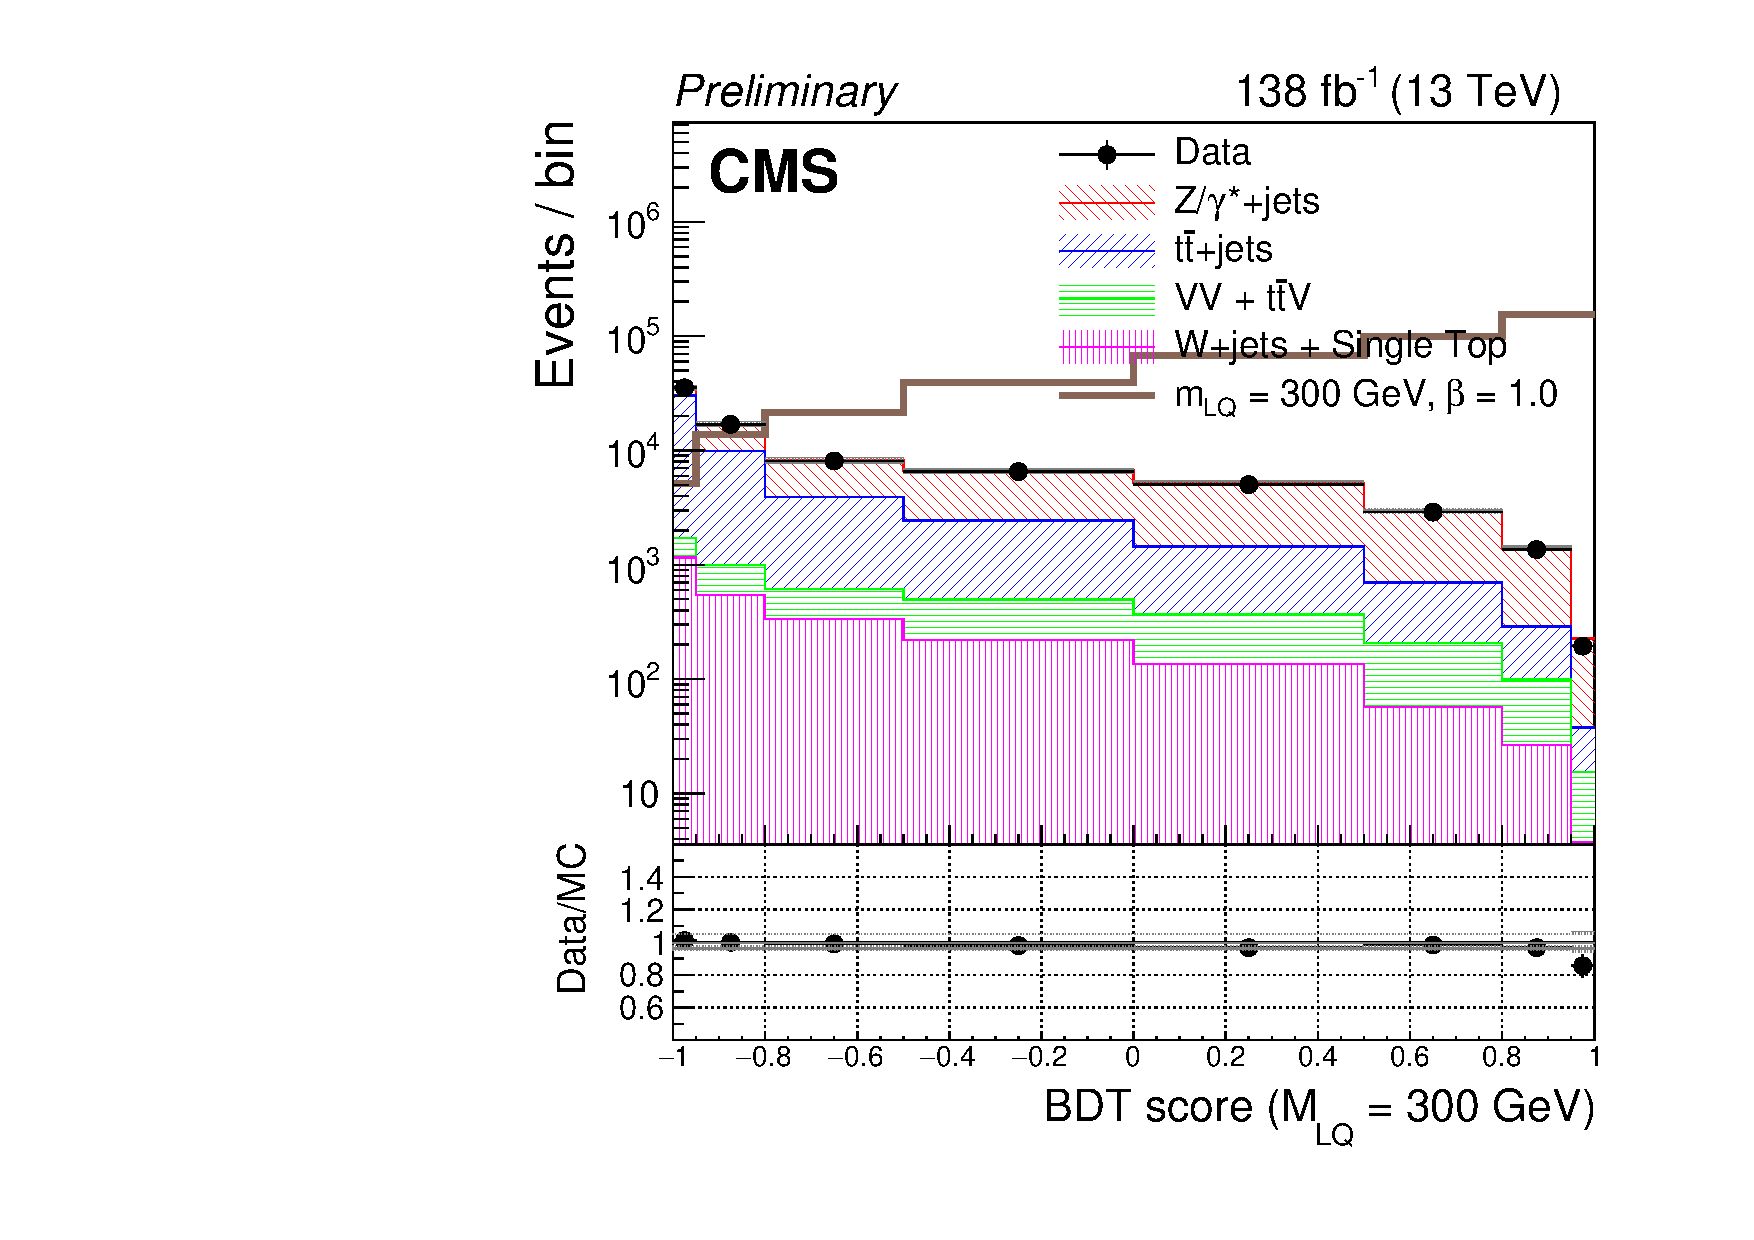
\includegraphics[width=.32\textwidth]{Images/Analysis/Results_combined_Unblinded/Plots/Preselection/BasicLQ_uujj_LQToBMu_pair_uubj_BDT_discrim_M300_standard.pdf}}
    {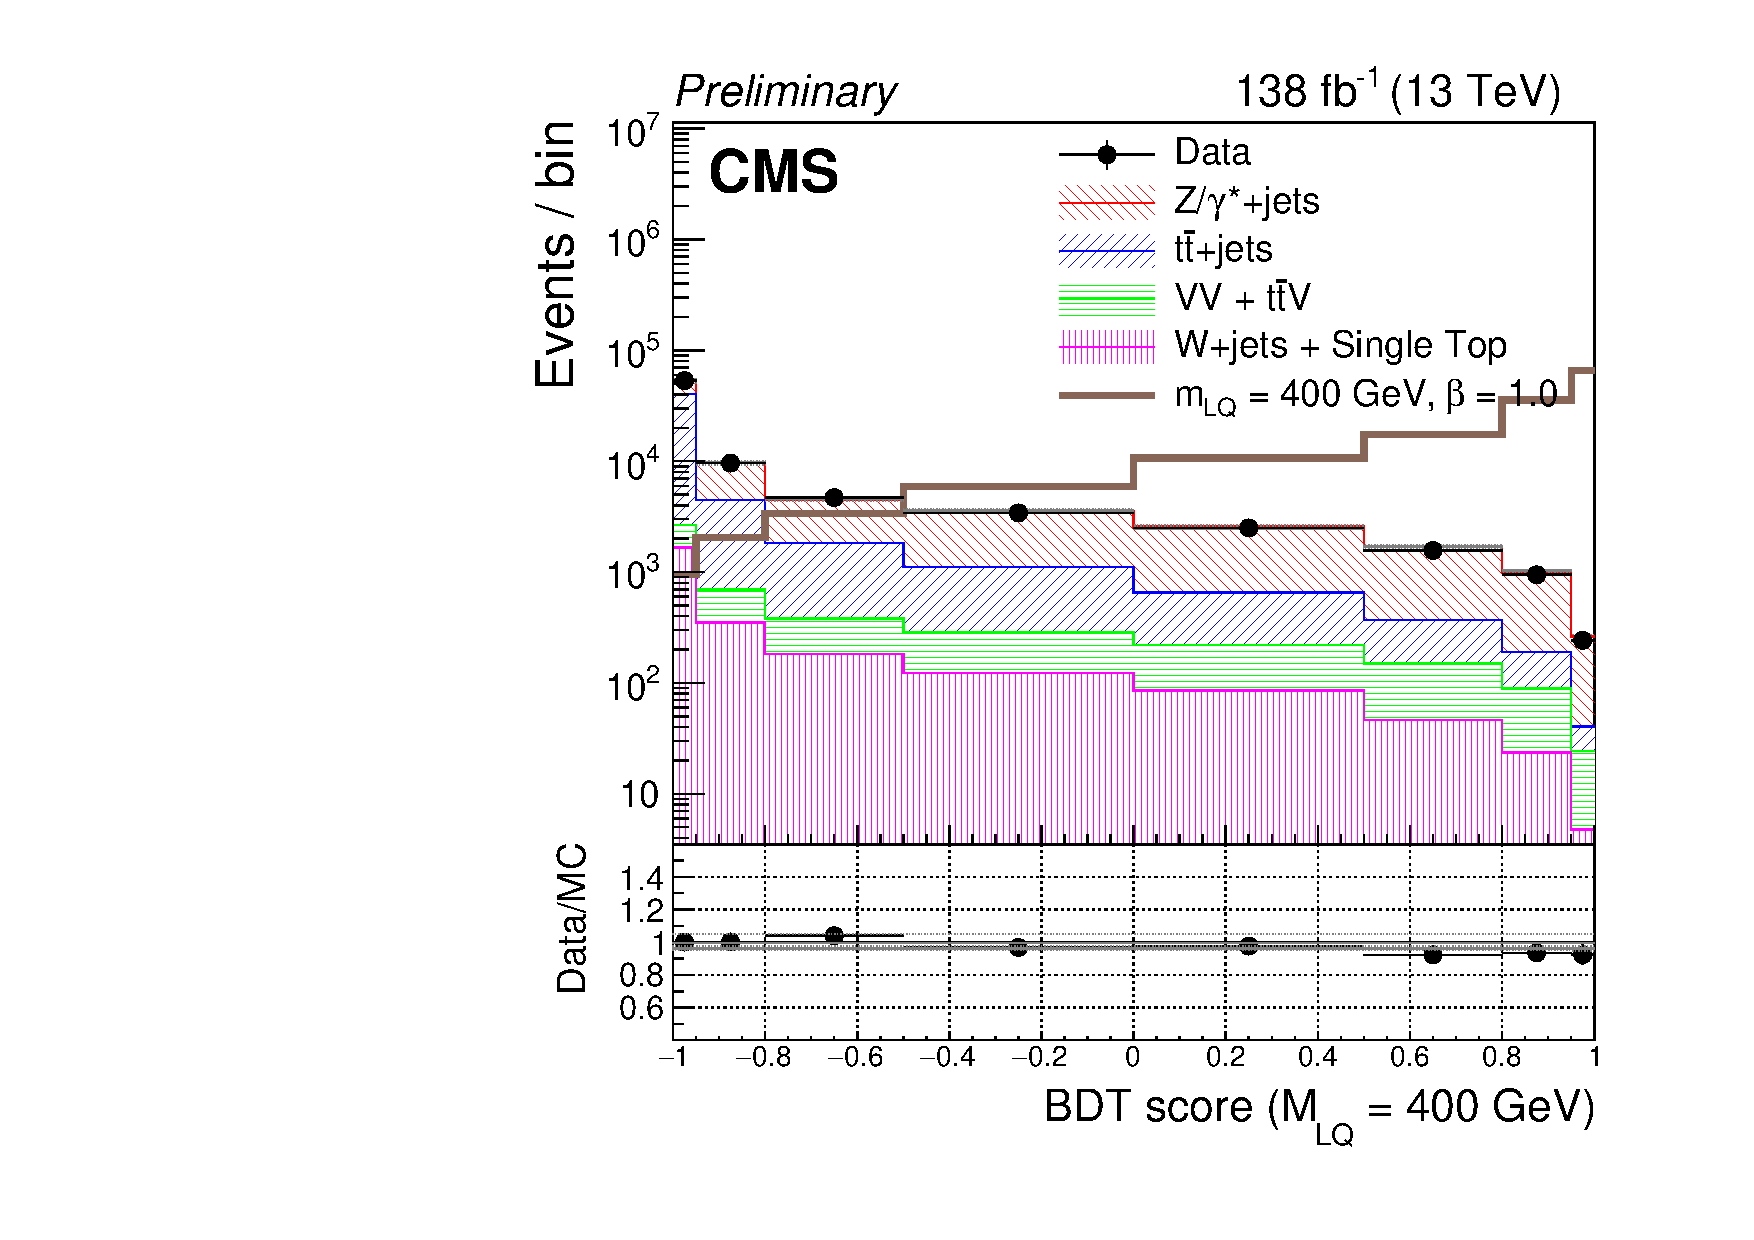
\includegraphics[width=.32\textwidth]{Images/Analysis/Results_combined_Unblinded/Plots/Preselection/BasicLQ_uujj_LQToBMu_pair_uubj_BDT_discrim_M400_standard.pdf}}
    {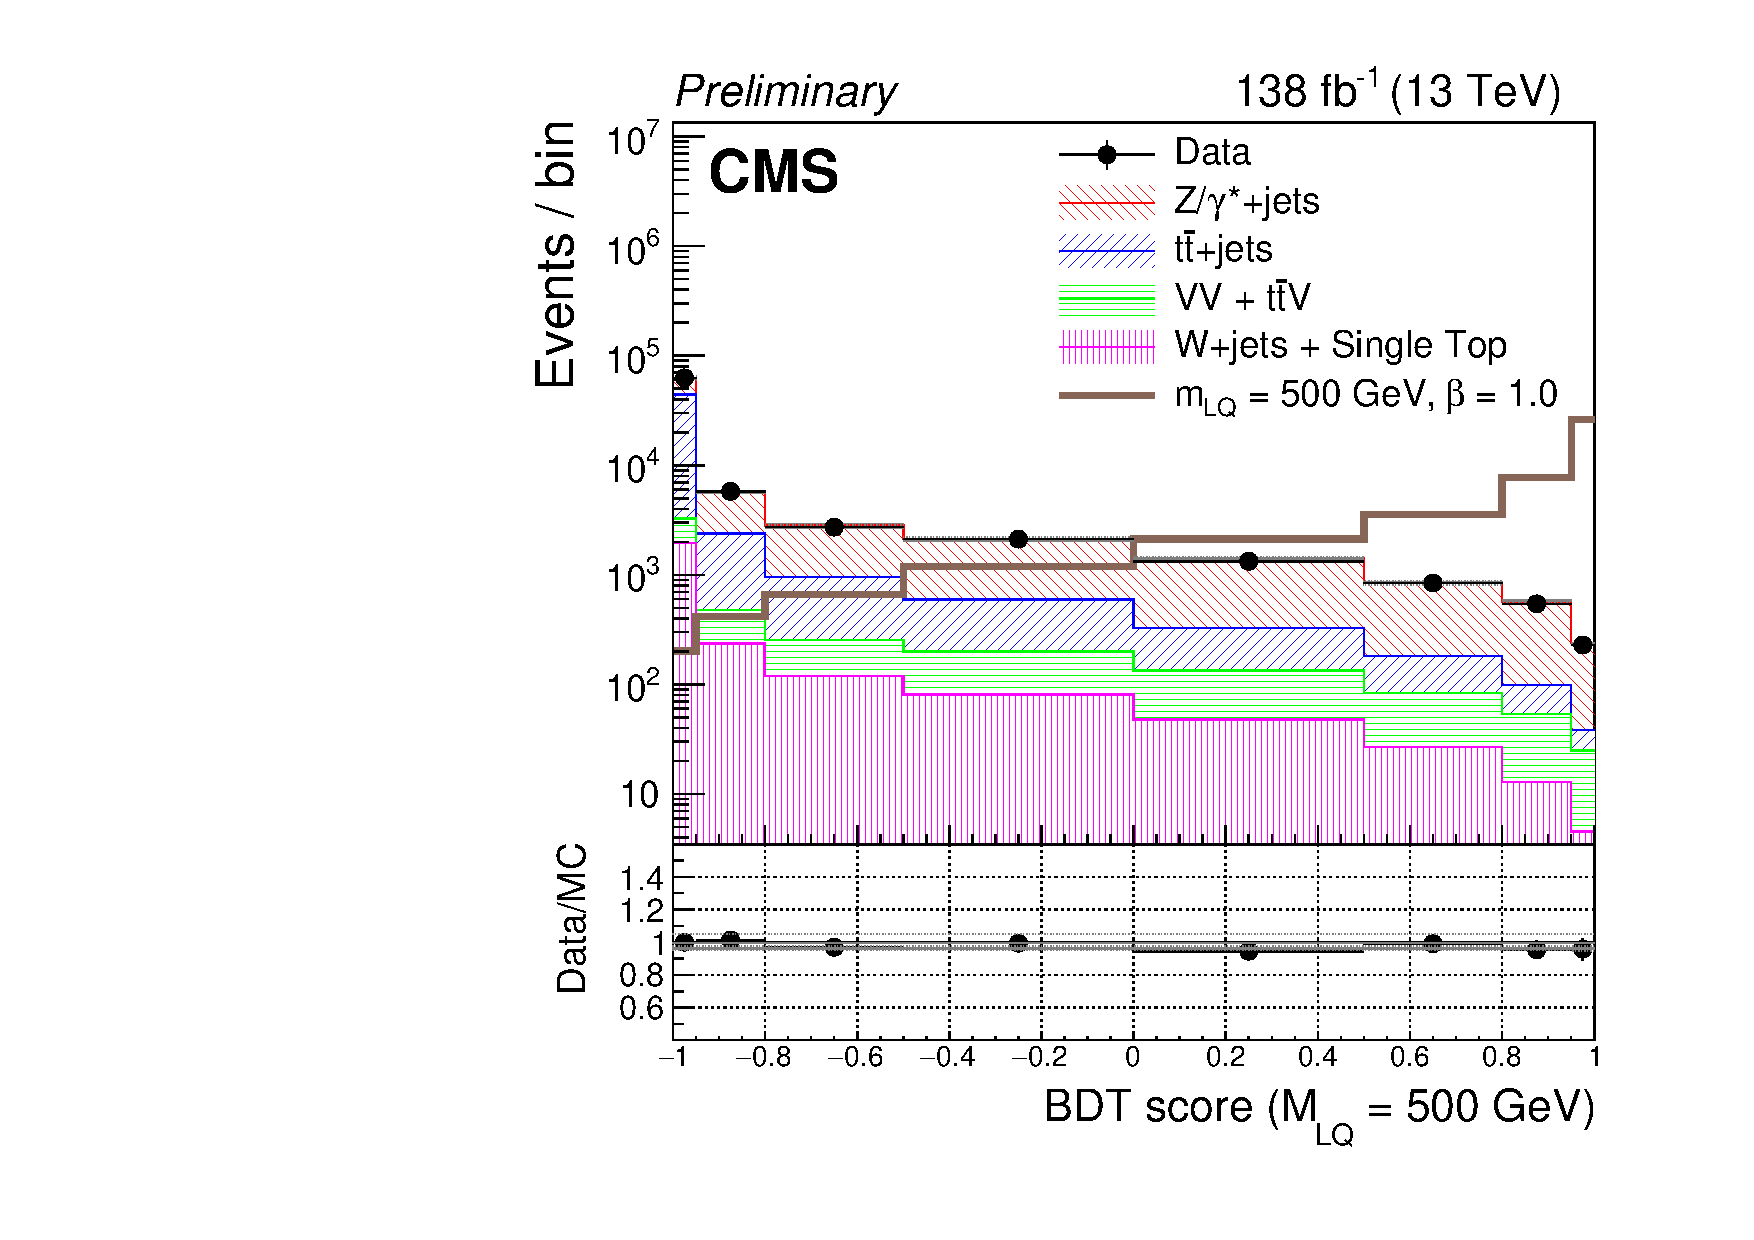
\includegraphics[width=.32\textwidth]{Images/Analysis/Results_combined_Unblinded/Plots/Preselection/BasicLQ_uujj_LQToBMu_pair_uubj_BDT_discrim_M500_standard.pdf}}
    {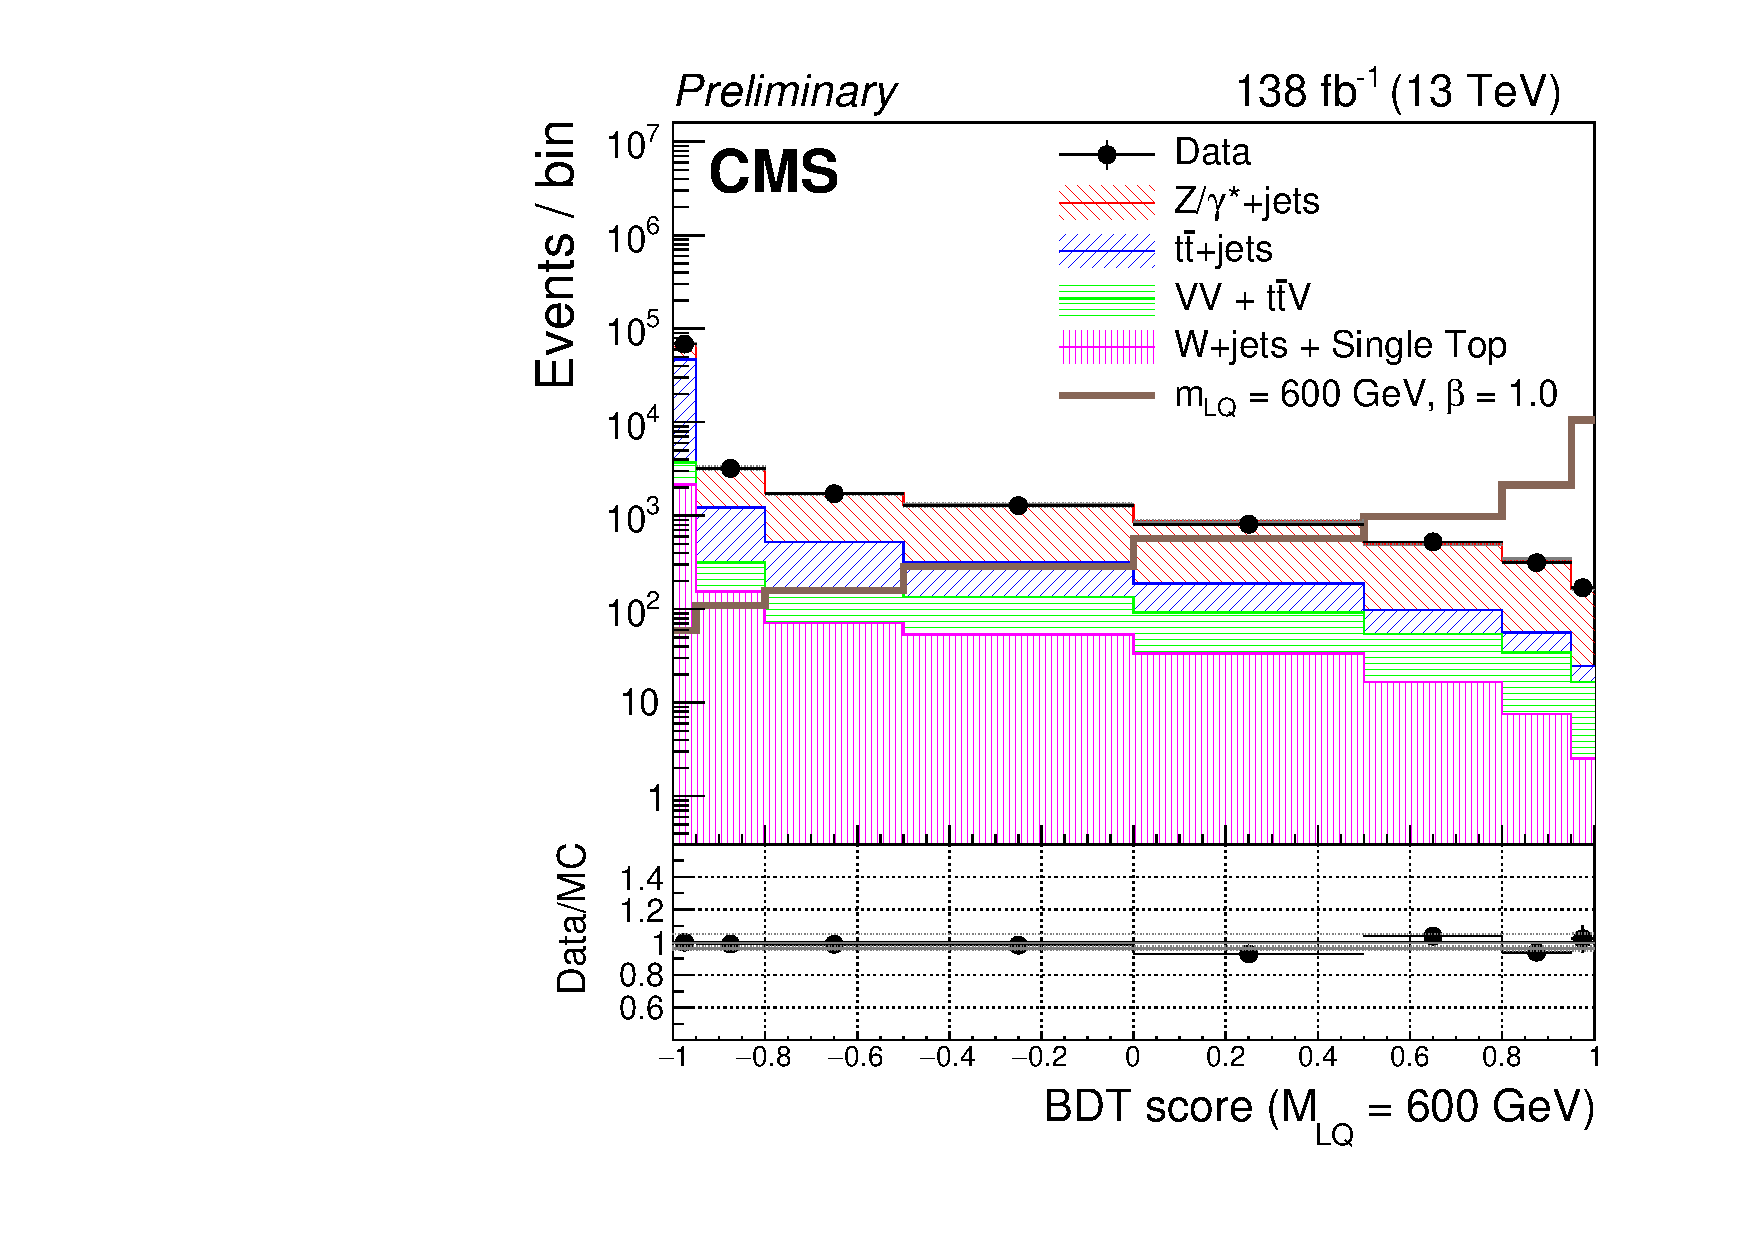
\includegraphics[width=.32\textwidth]{Images/Analysis/Results_combined_Unblinded/Plots/Preselection/BasicLQ_uujj_LQToBMu_pair_uubj_BDT_discrim_M600_standard.pdf}}
    {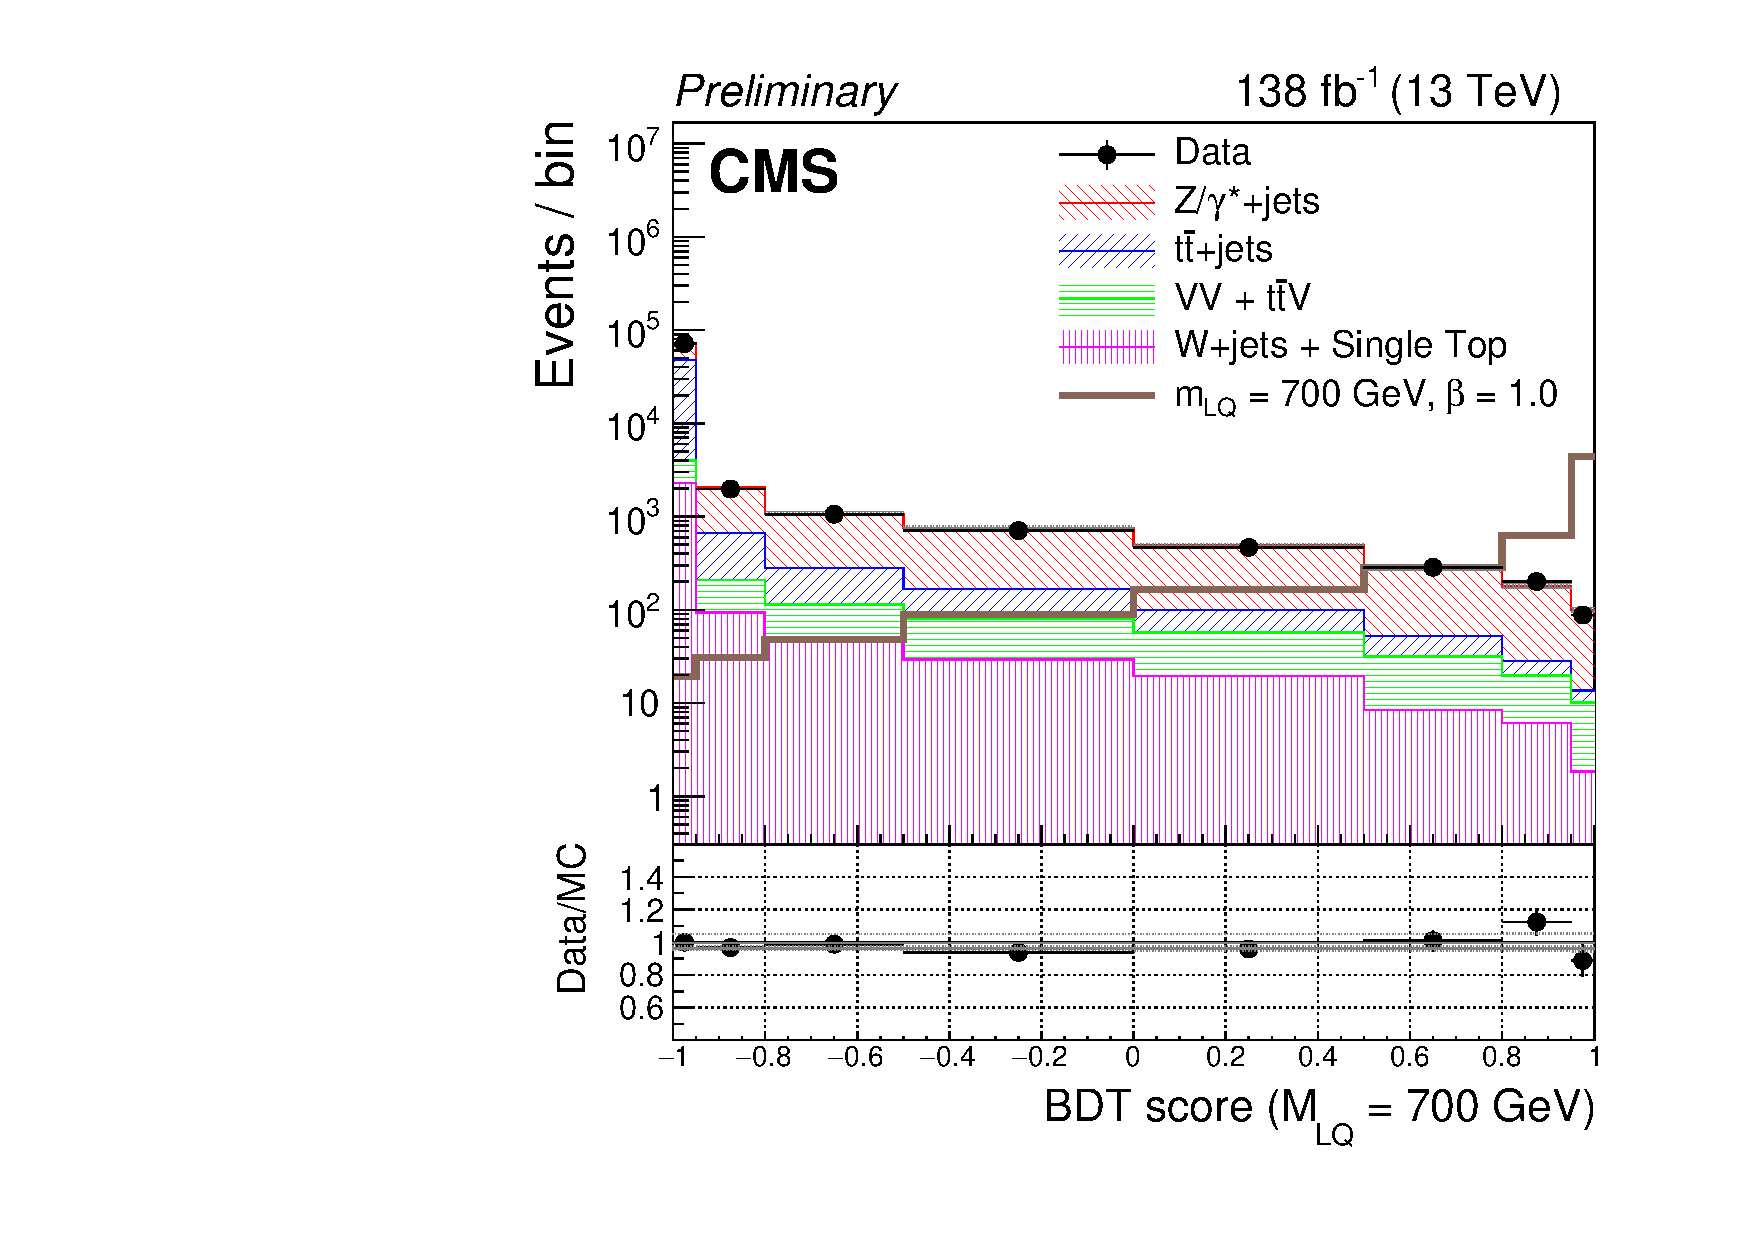
\includegraphics[width=.32\textwidth]{Images/Analysis/Results_combined_Unblinded/Plots/Preselection/BasicLQ_uujj_LQToBMu_pair_uubj_BDT_discrim_M700_standard.pdf}}
    {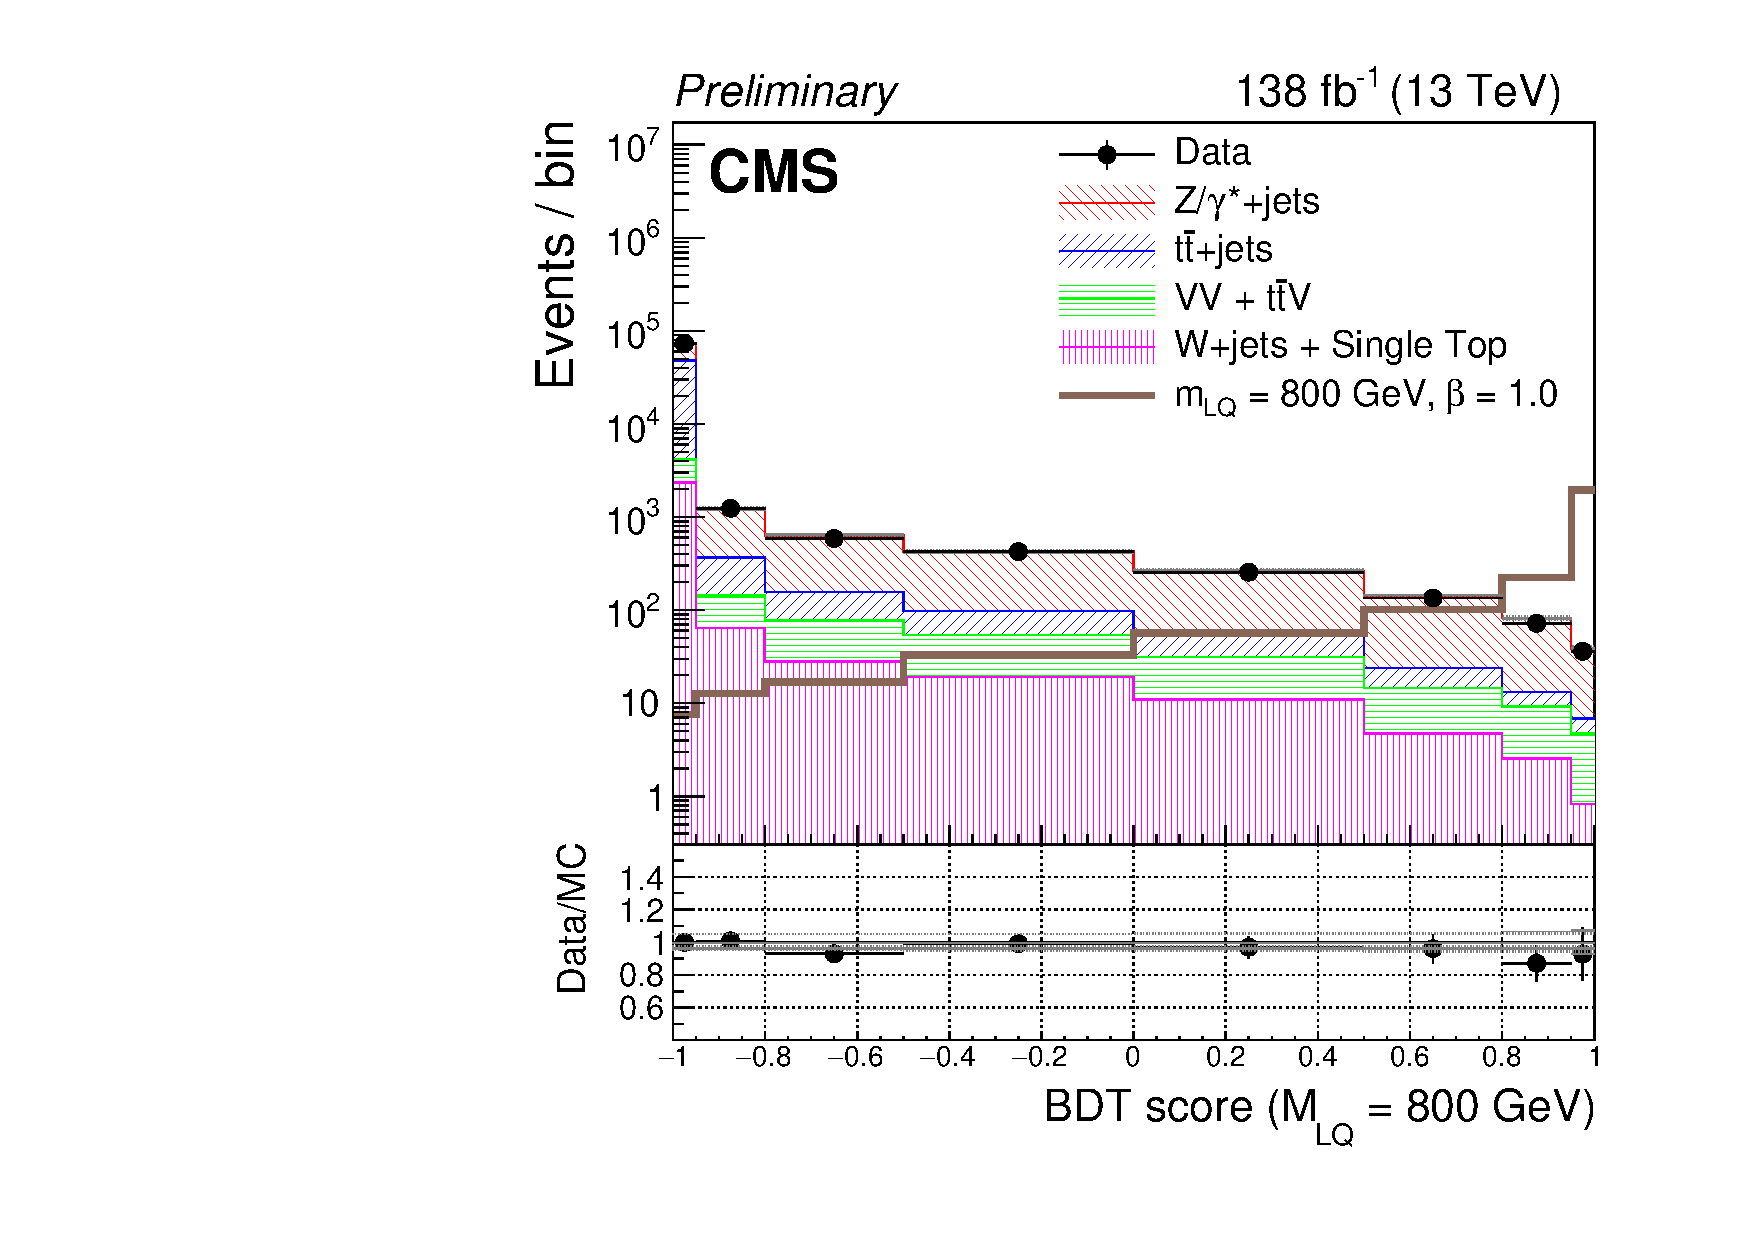
\includegraphics[width=.32\textwidth]{Images/Analysis/Results_combined_Unblinded/Plots/Preselection/BasicLQ_uujj_LQToBMu_pair_uubj_BDT_discrim_M800_standard.pdf}}
    {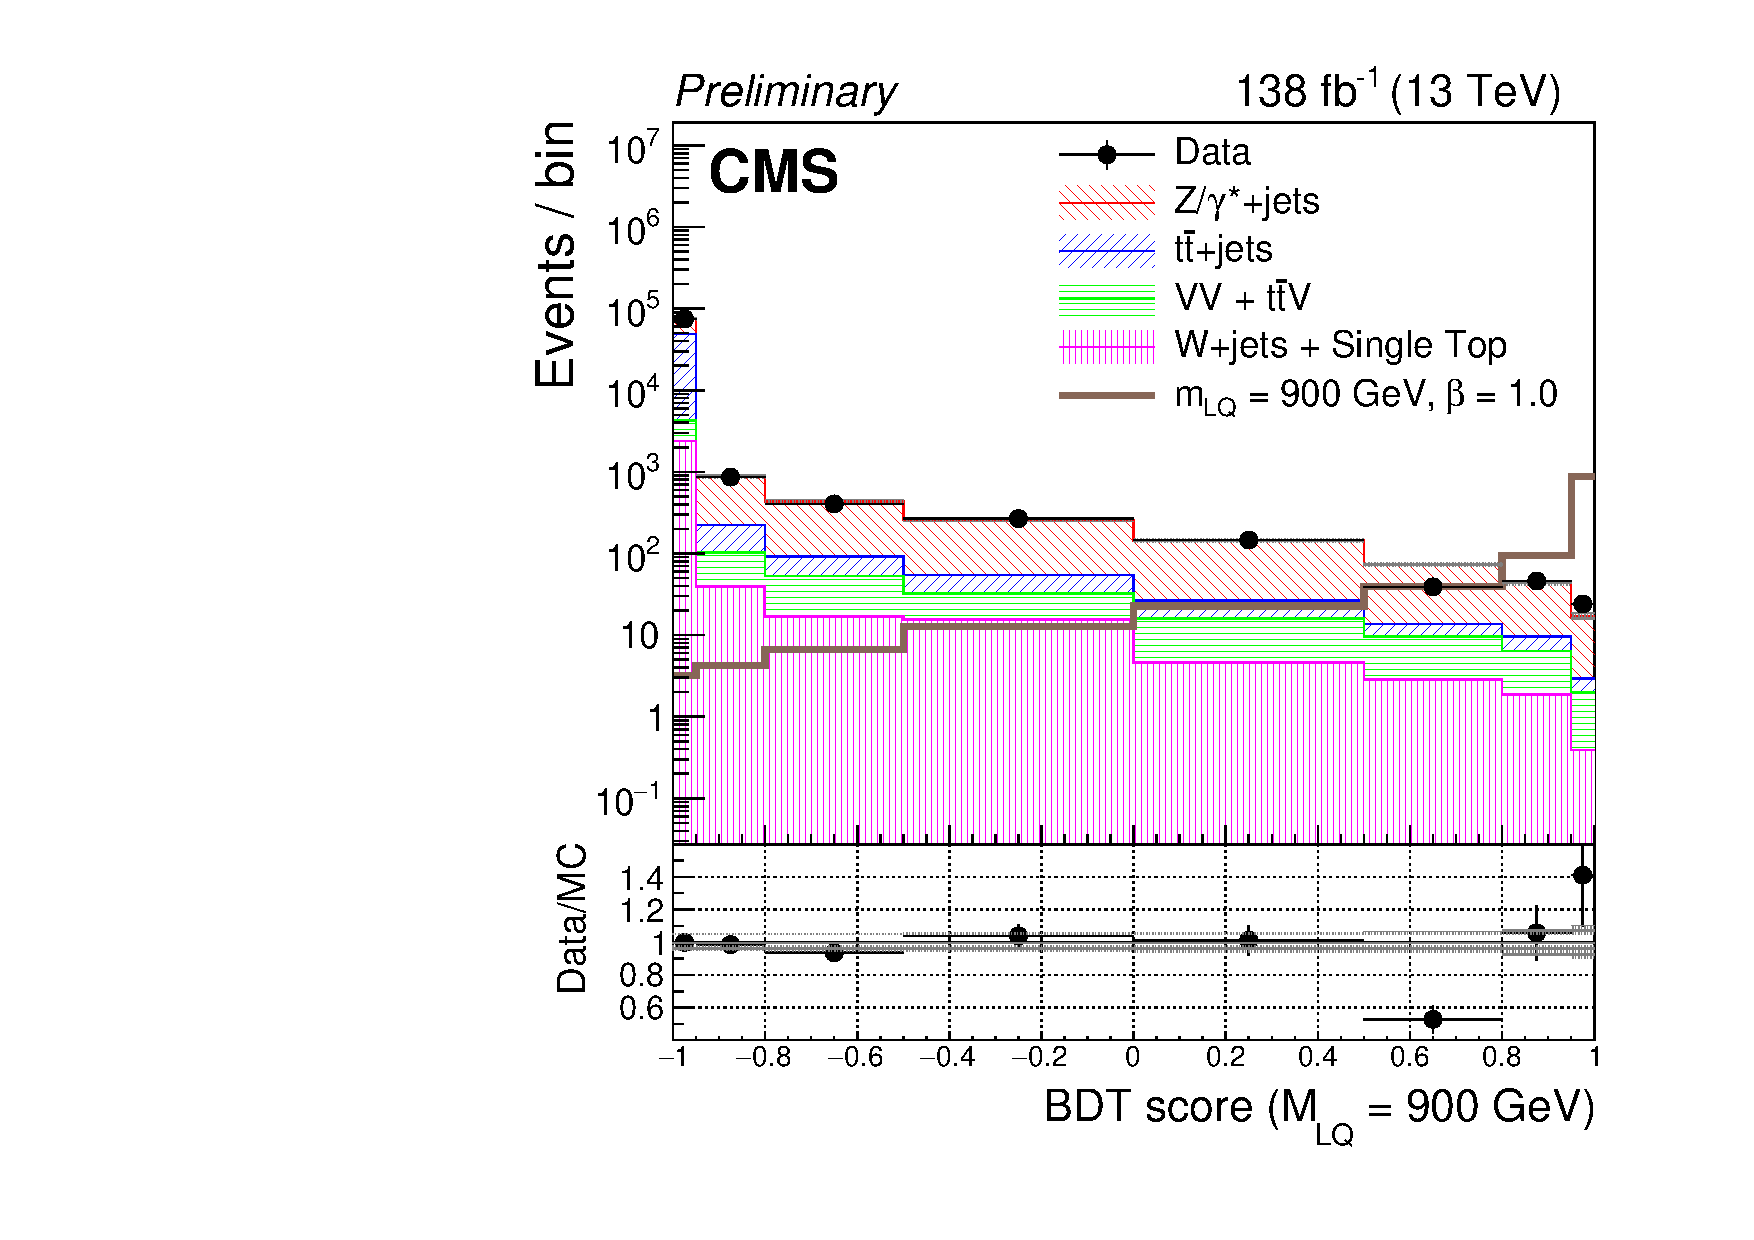
\includegraphics[width=.32\textwidth]{Images/Analysis/Results_combined_Unblinded/Plots/Preselection/BasicLQ_uujj_LQToBMu_pair_uubj_BDT_discrim_M900_standard.pdf}}
    {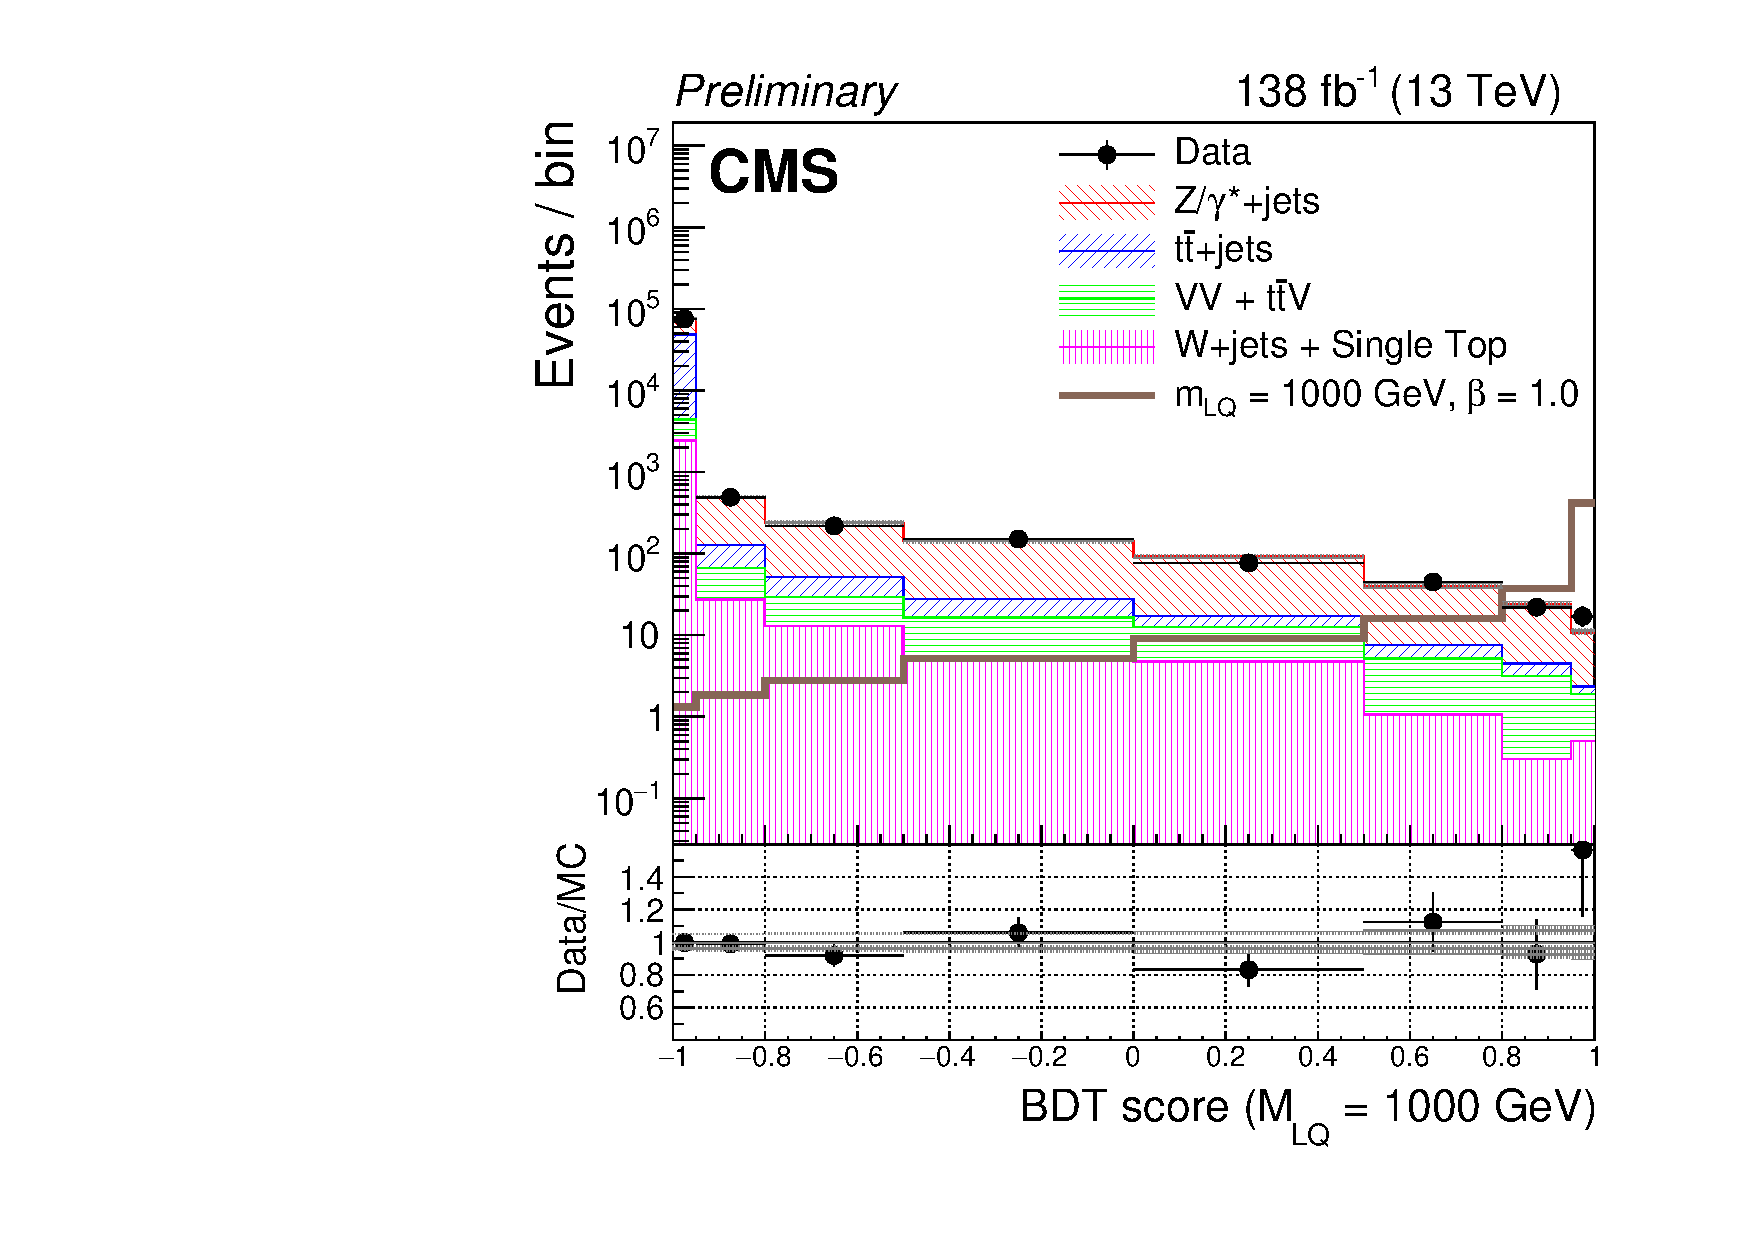
\includegraphics[width=.32\textwidth]{Images/Analysis/Results_combined_Unblinded/Plots/Preselection/BasicLQ_uujj_LQToBMu_pair_uubj_BDT_discrim_M1000_standard.pdf}}
    {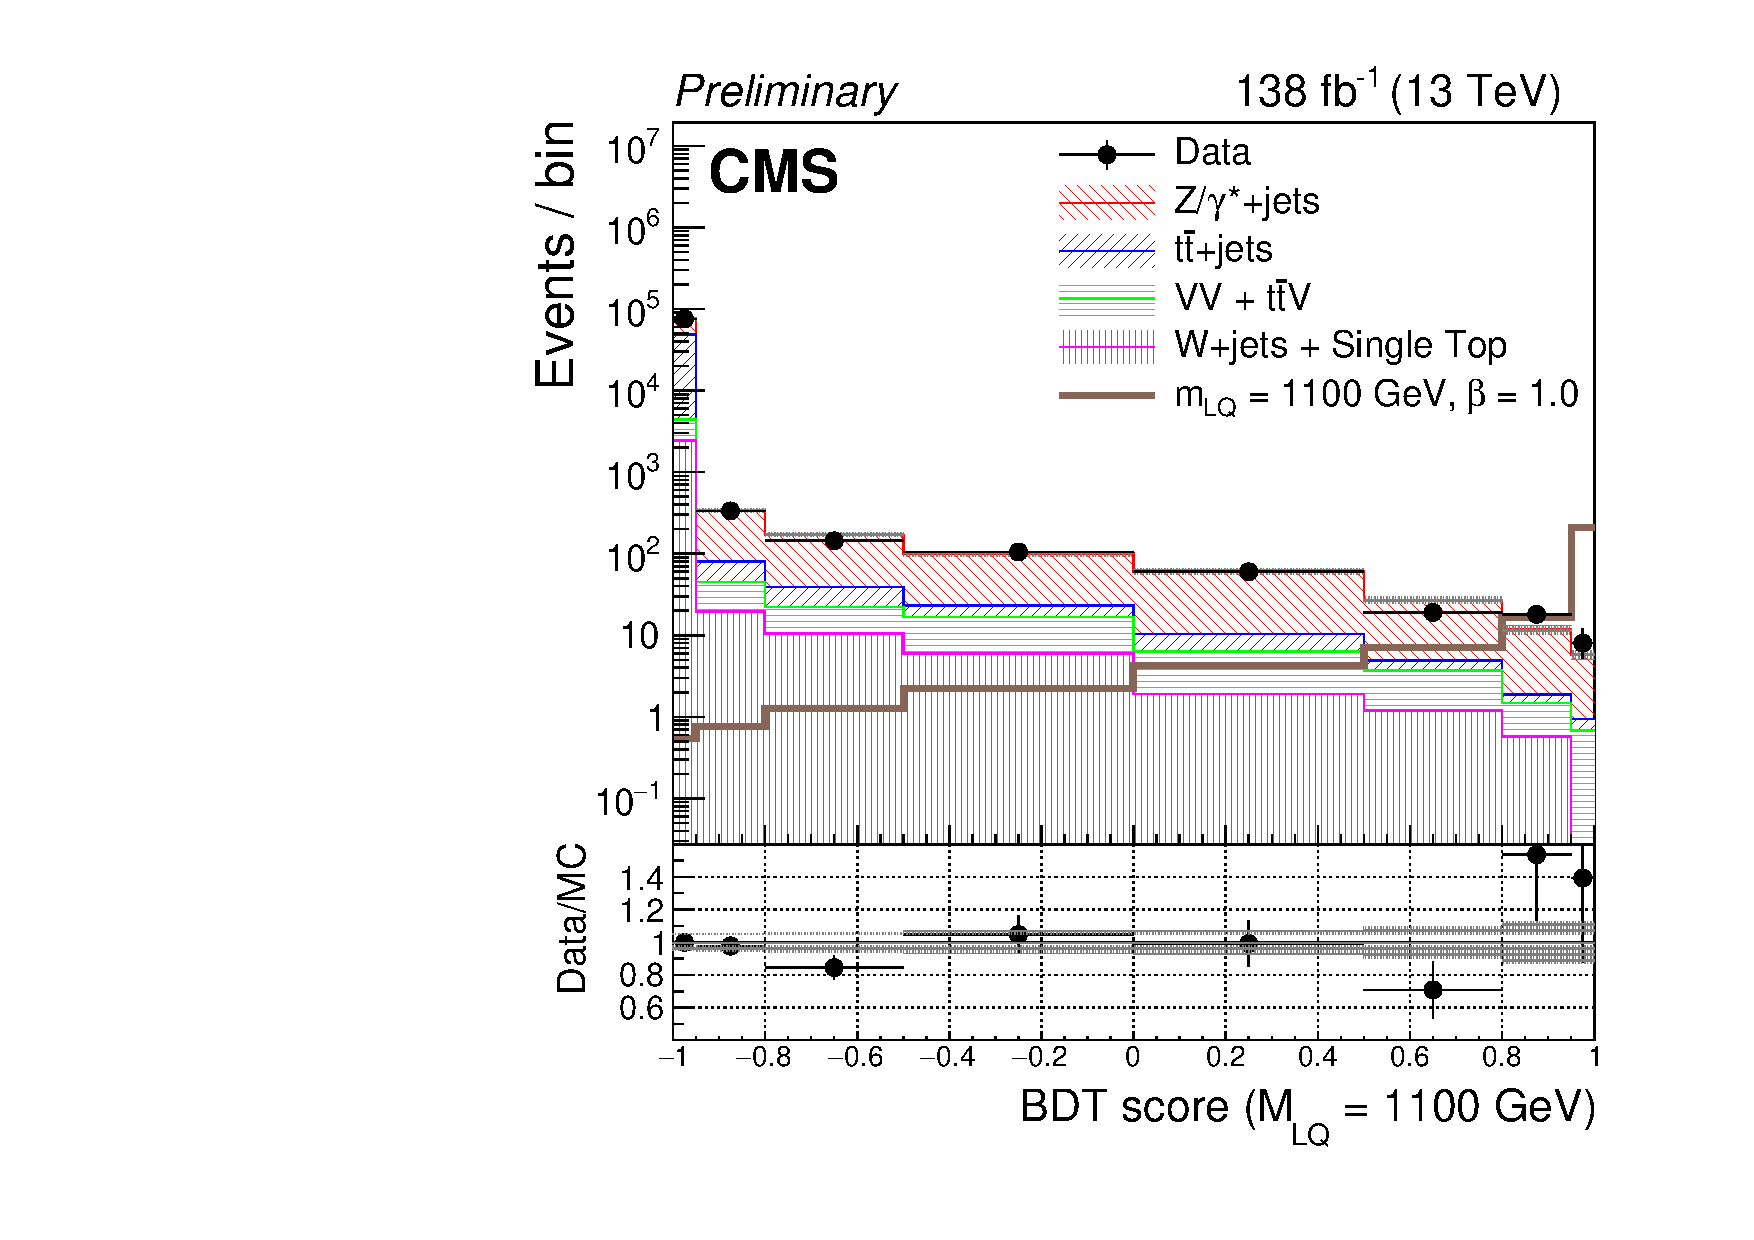
\includegraphics[width=.32\textwidth]{Images/Analysis/Results_combined_Unblinded/Plots/Preselection/BasicLQ_uujj_LQToBMu_pair_uubj_BDT_discrim_M1100_standard.pdf}}
    {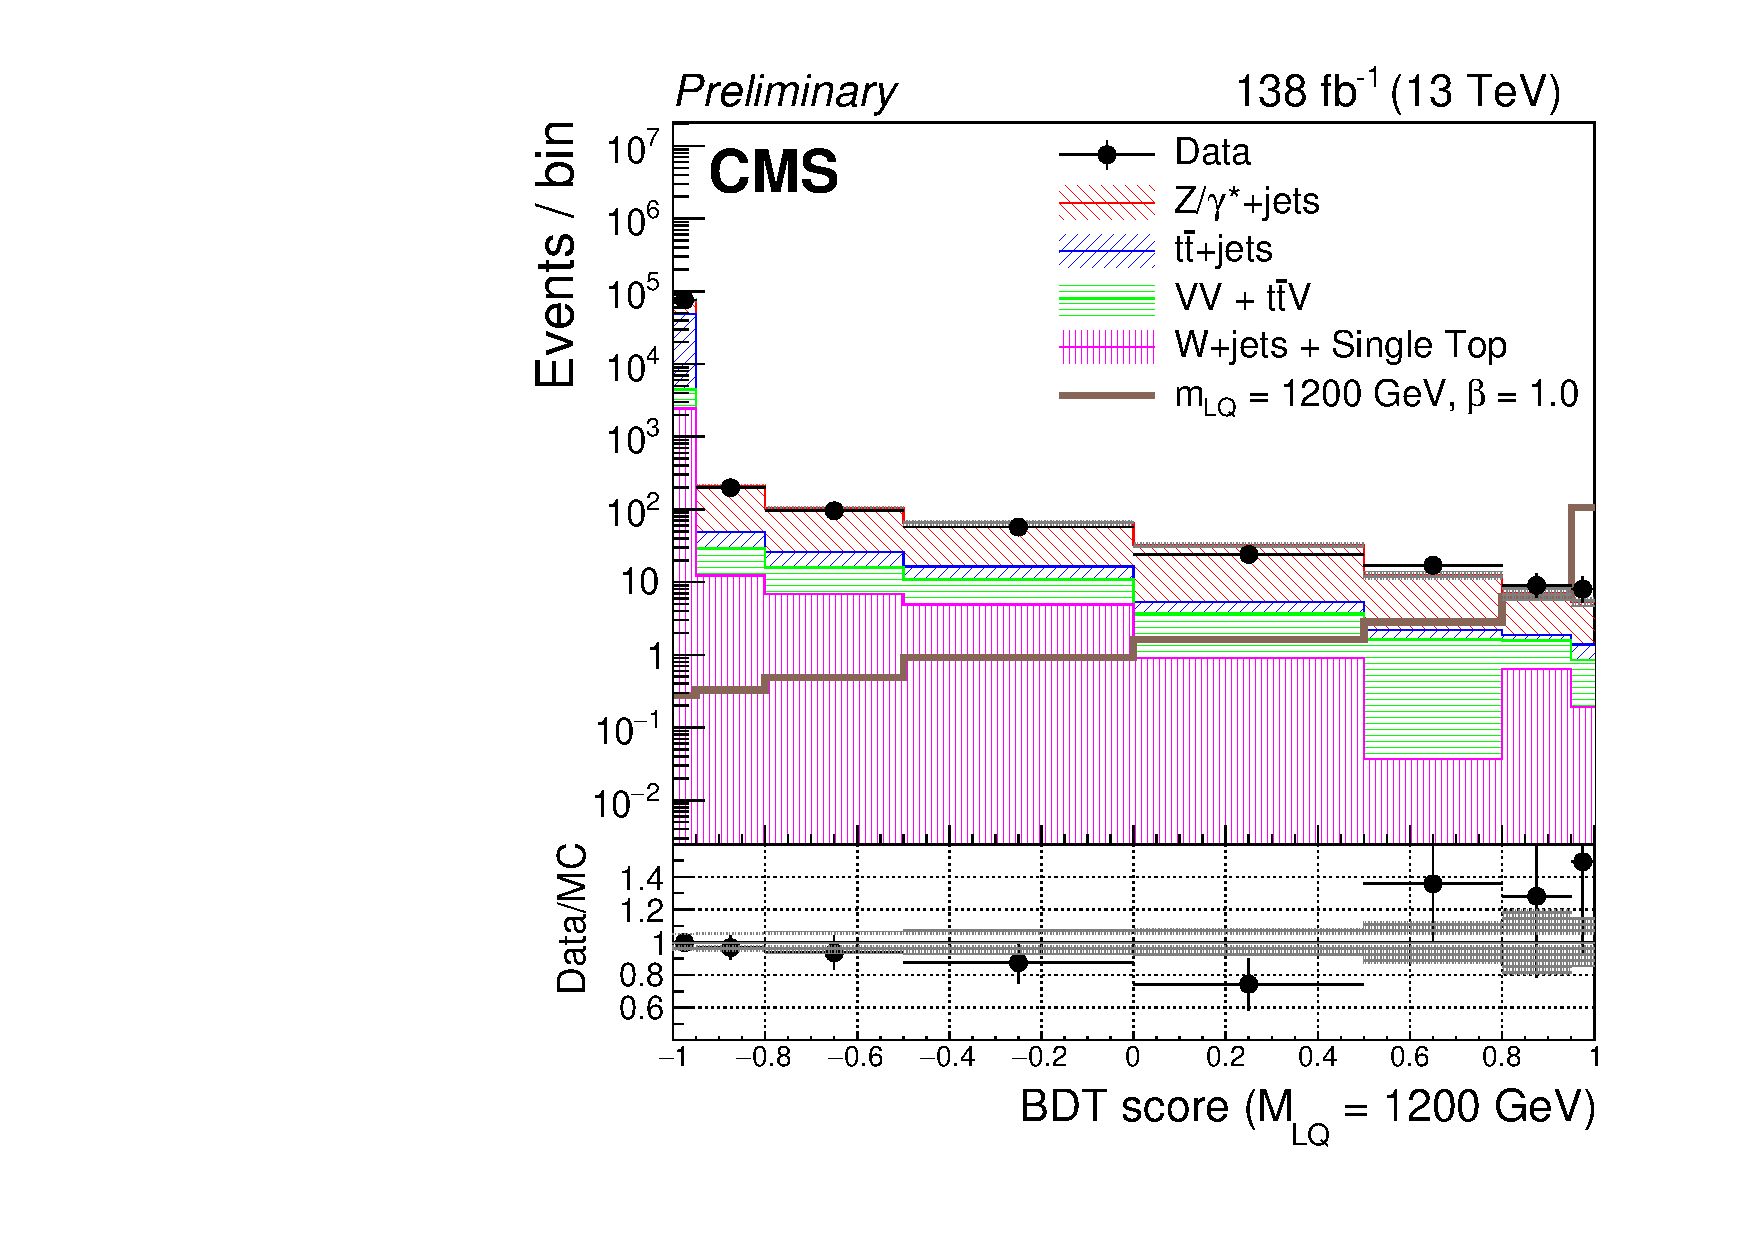
\includegraphics[width=.32\textwidth]{Images/Analysis/Results_combined_Unblinded/Plots/Preselection/BasicLQ_uujj_LQToBMu_pair_uubj_BDT_discrim_M1200_standard.pdf}}
    {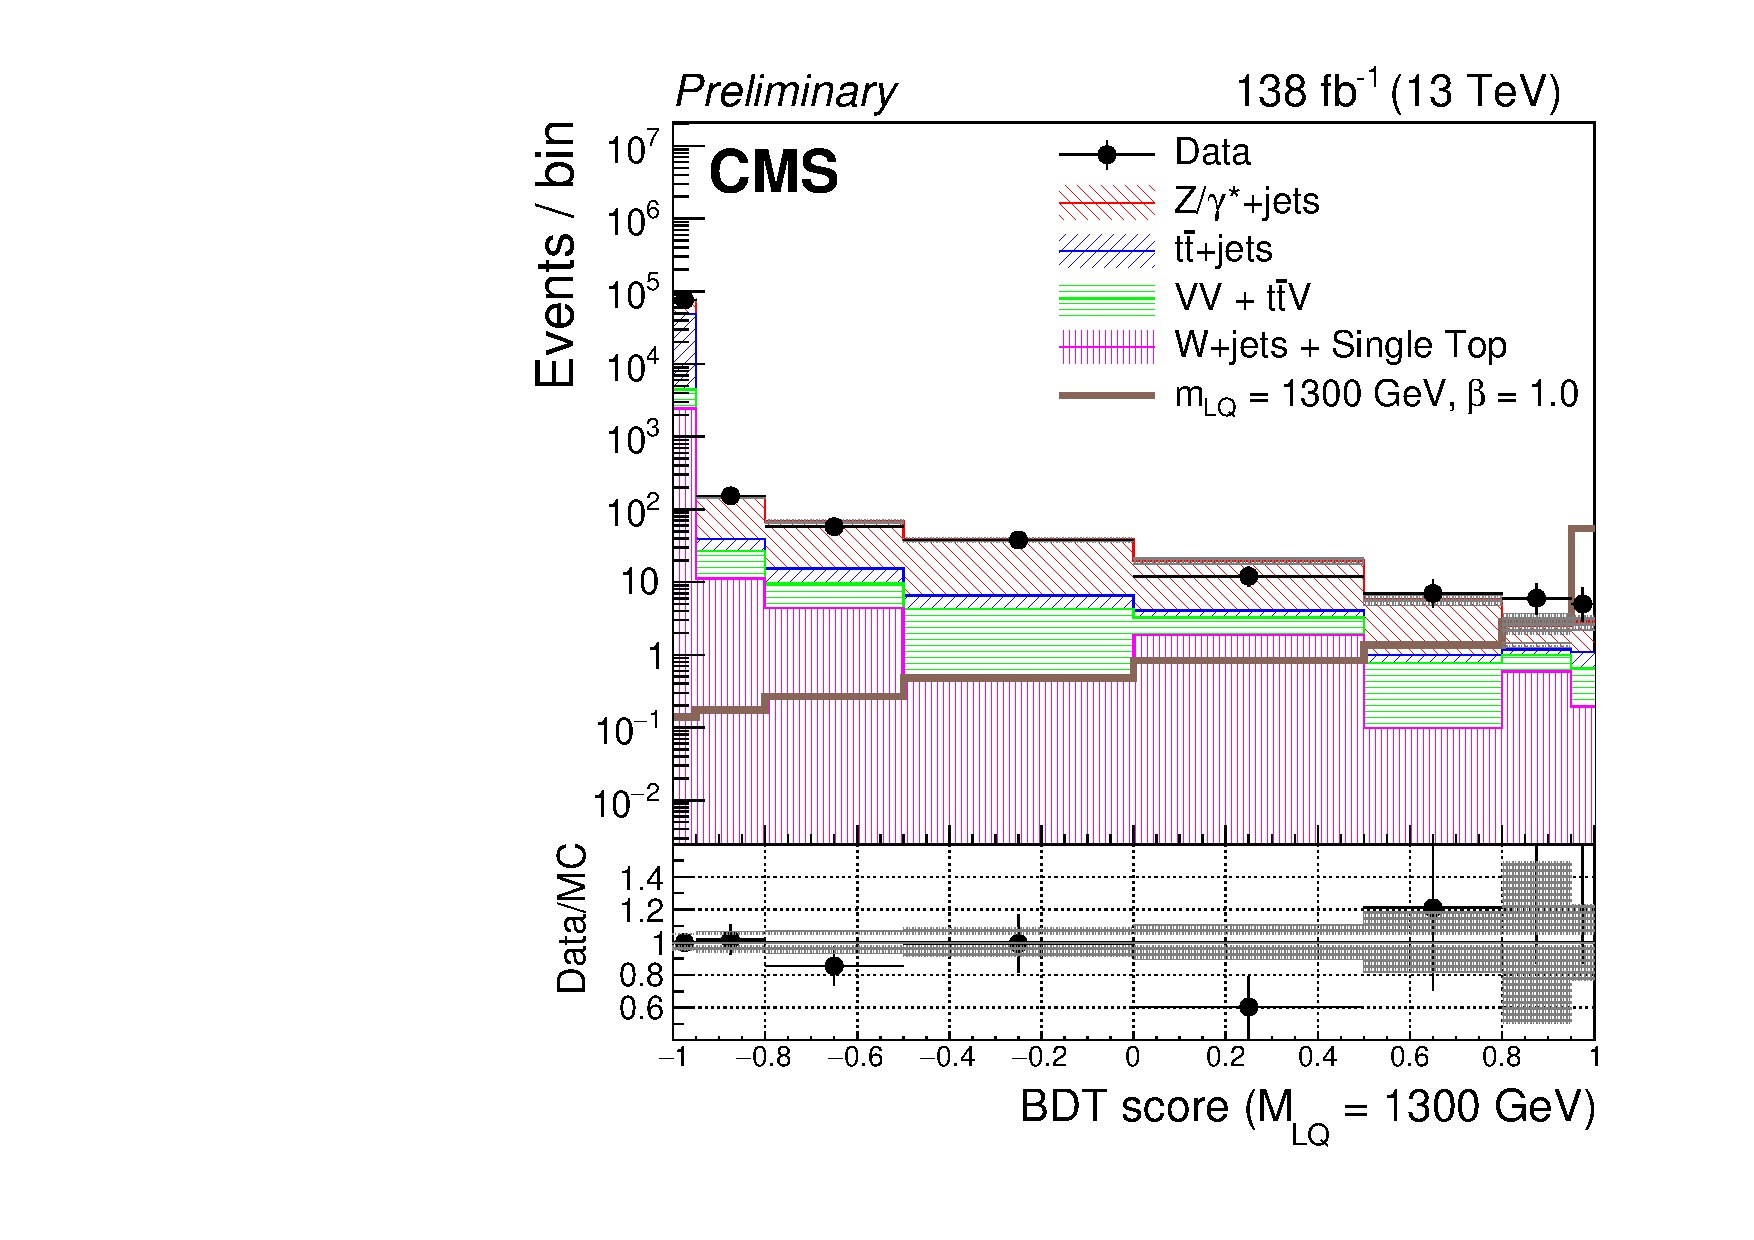
\includegraphics[width=.32\textwidth]{Images/Analysis/Results_combined_Unblinded/Plots/Preselection/BasicLQ_uujj_LQToBMu_pair_uubj_BDT_discrim_M1300_standard.pdf}}
    {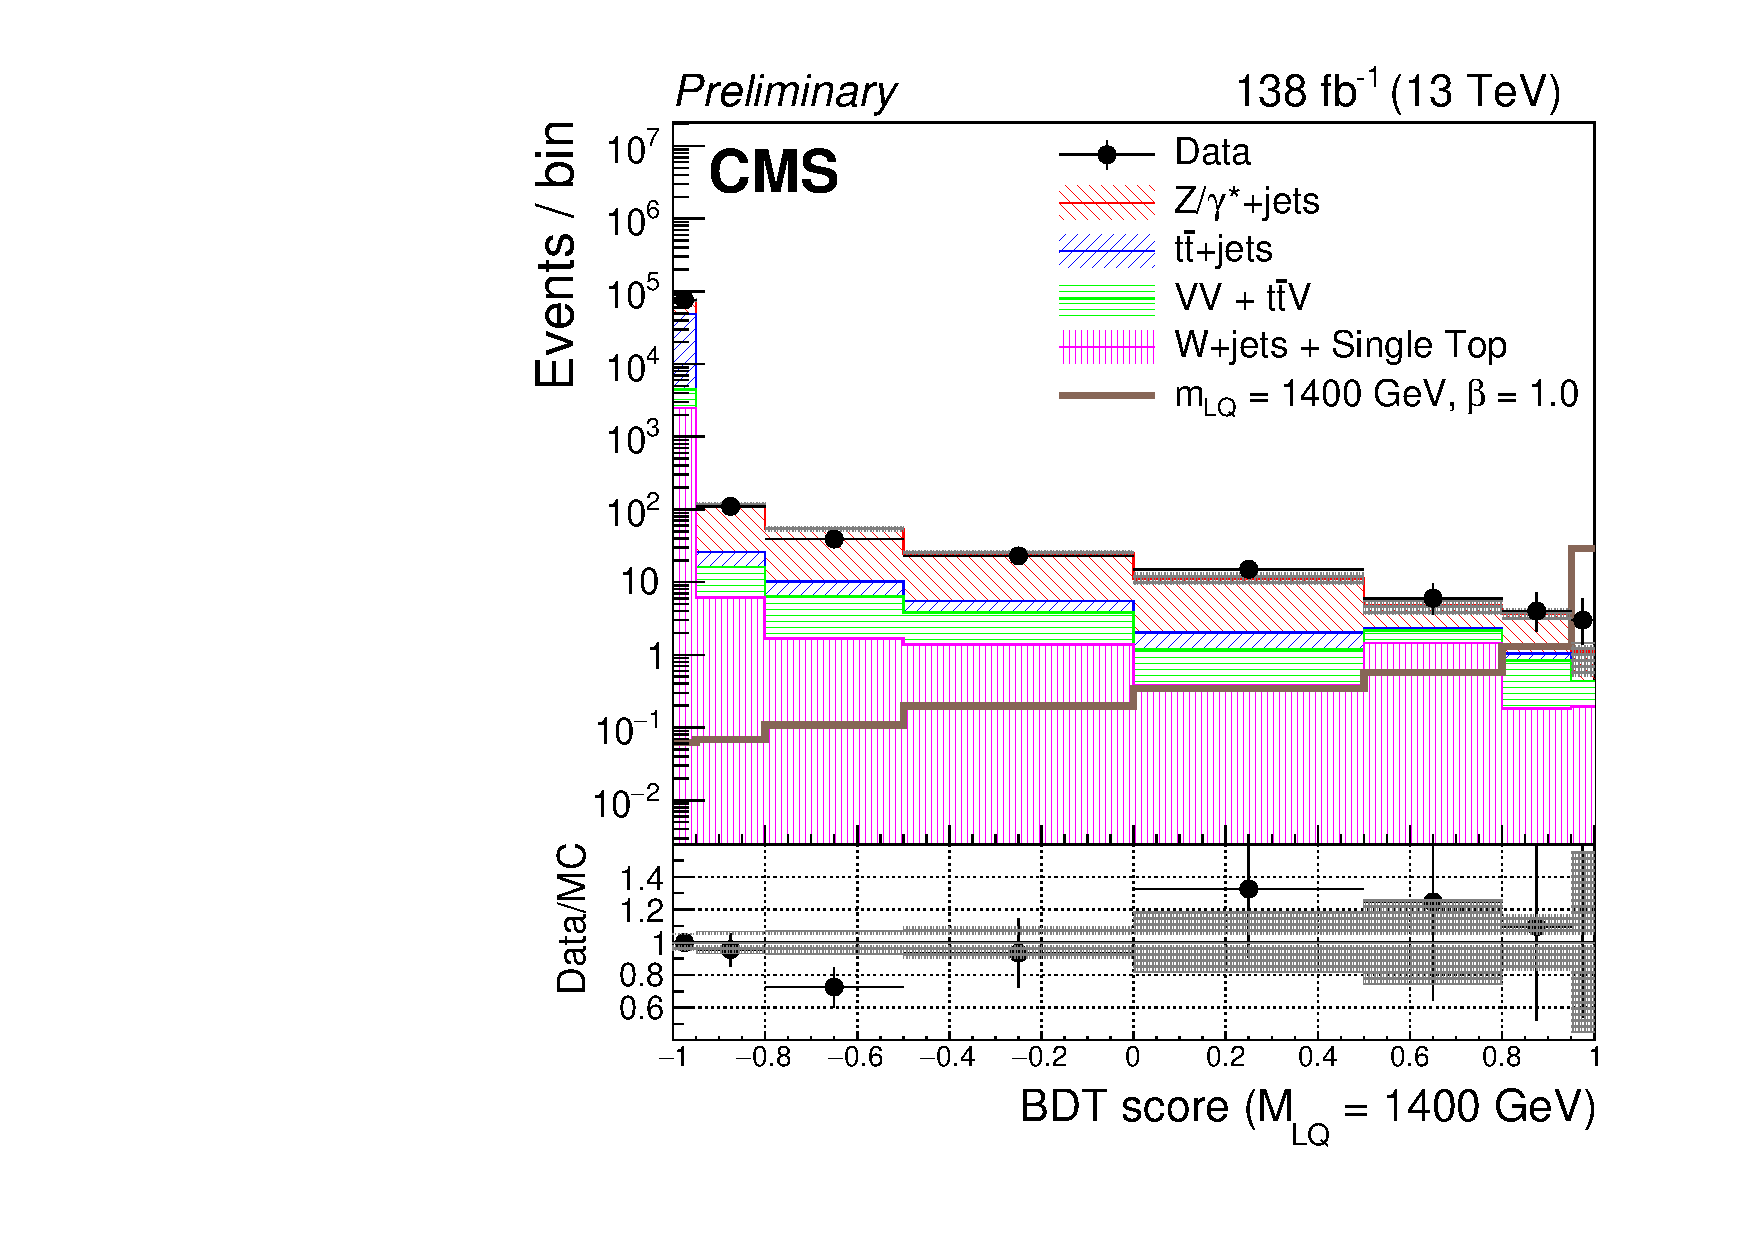
\includegraphics[width=.32\textwidth]{Images/Analysis/Results_combined_Unblinded/Plots/Preselection/BasicLQ_uujj_LQToBMu_pair_uubj_BDT_discrim_M1400_standard.pdf}}

    \caption{A comparison between observed and expected events in BDT responses at preselection level with the combination of 2016, 2017, and 2018 data. The leptoquark mass of the signal in each plot corresponds to the leptoquark mass used in the BDT training. Error bars represent statistical uncertainties, while the shaded area represents systematic uncertainties.
    \label{figapp:BDT300to1400}}
\end{figure}

\begin{figure}[H]
    \centering
    {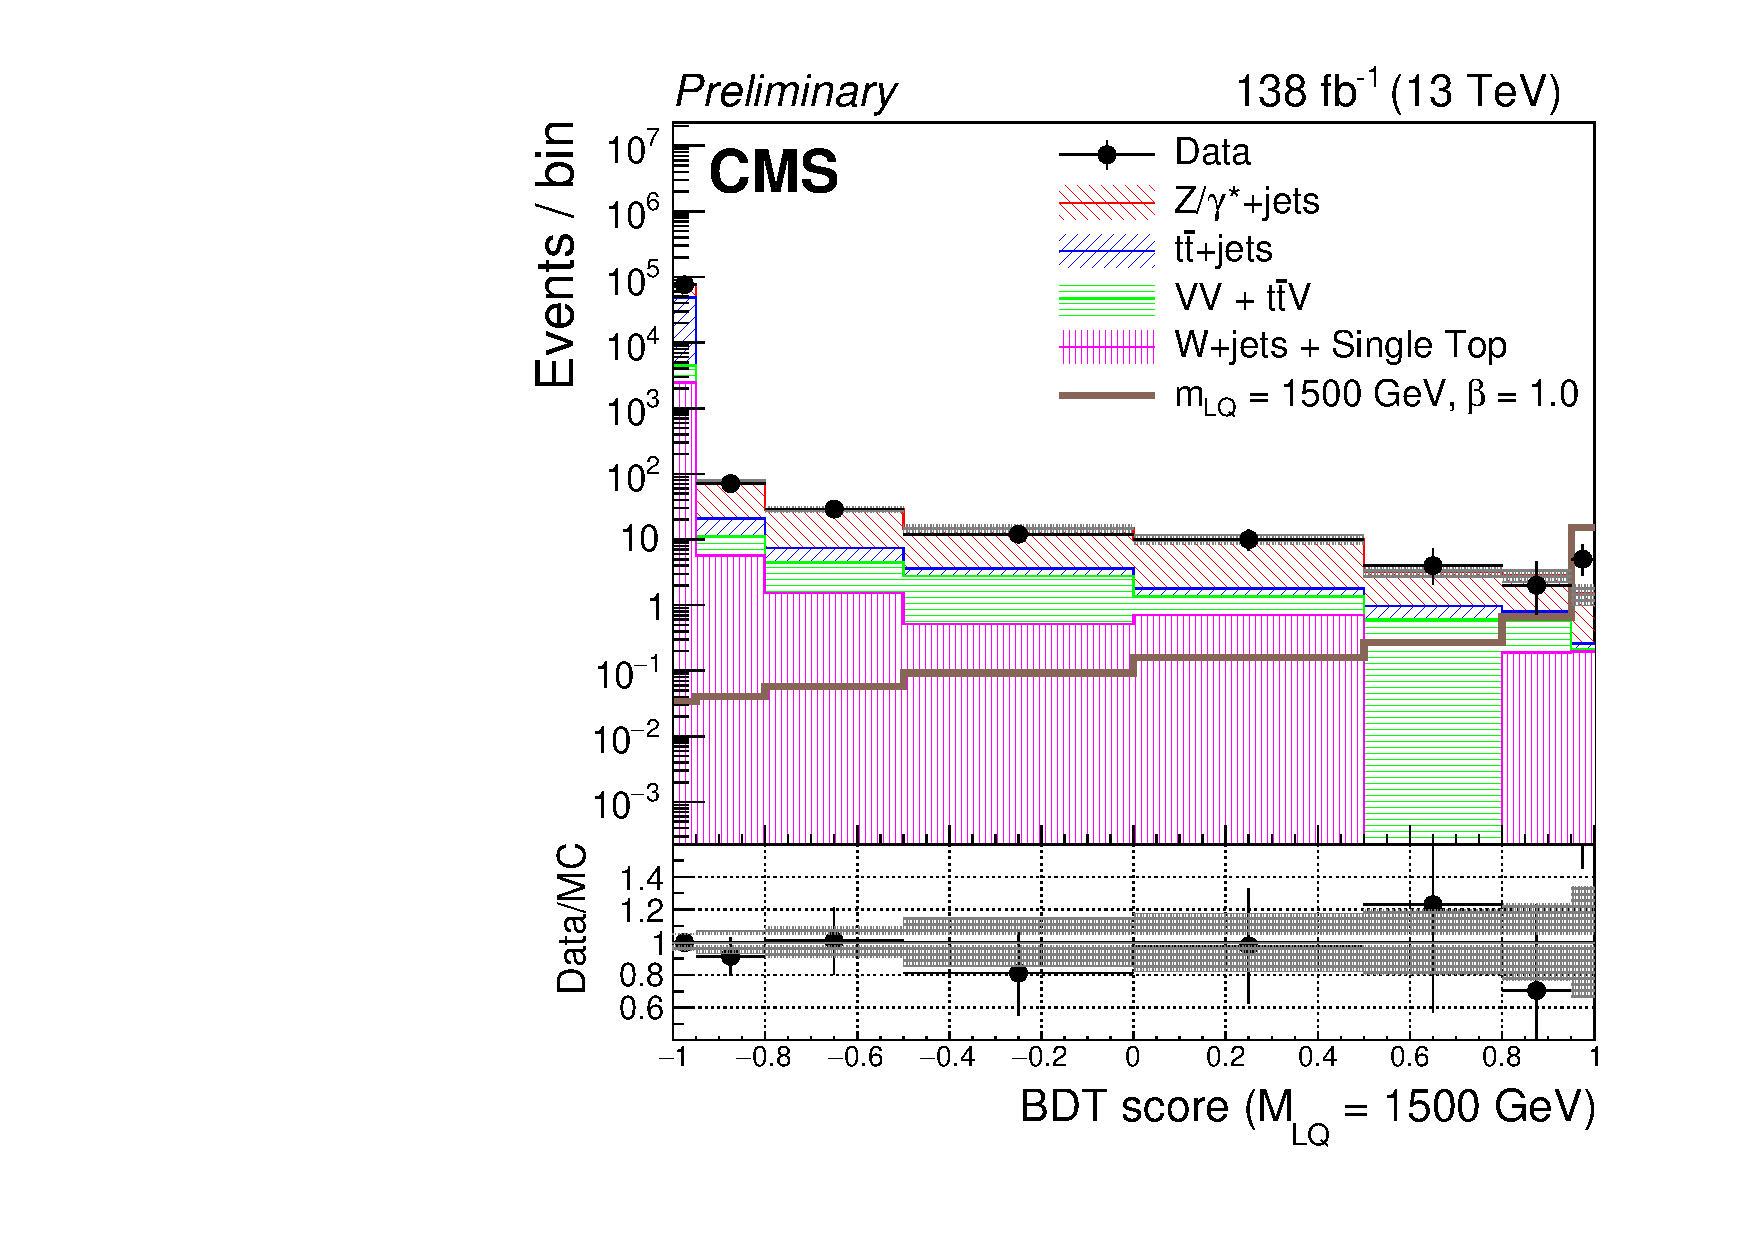
\includegraphics[width=.32\textwidth]{Images/Analysis/Results_combined_Unblinded/Plots/Preselection/BasicLQ_uujj_LQToBMu_pair_uubj_BDT_discrim_M1500_standard.pdf}}
    {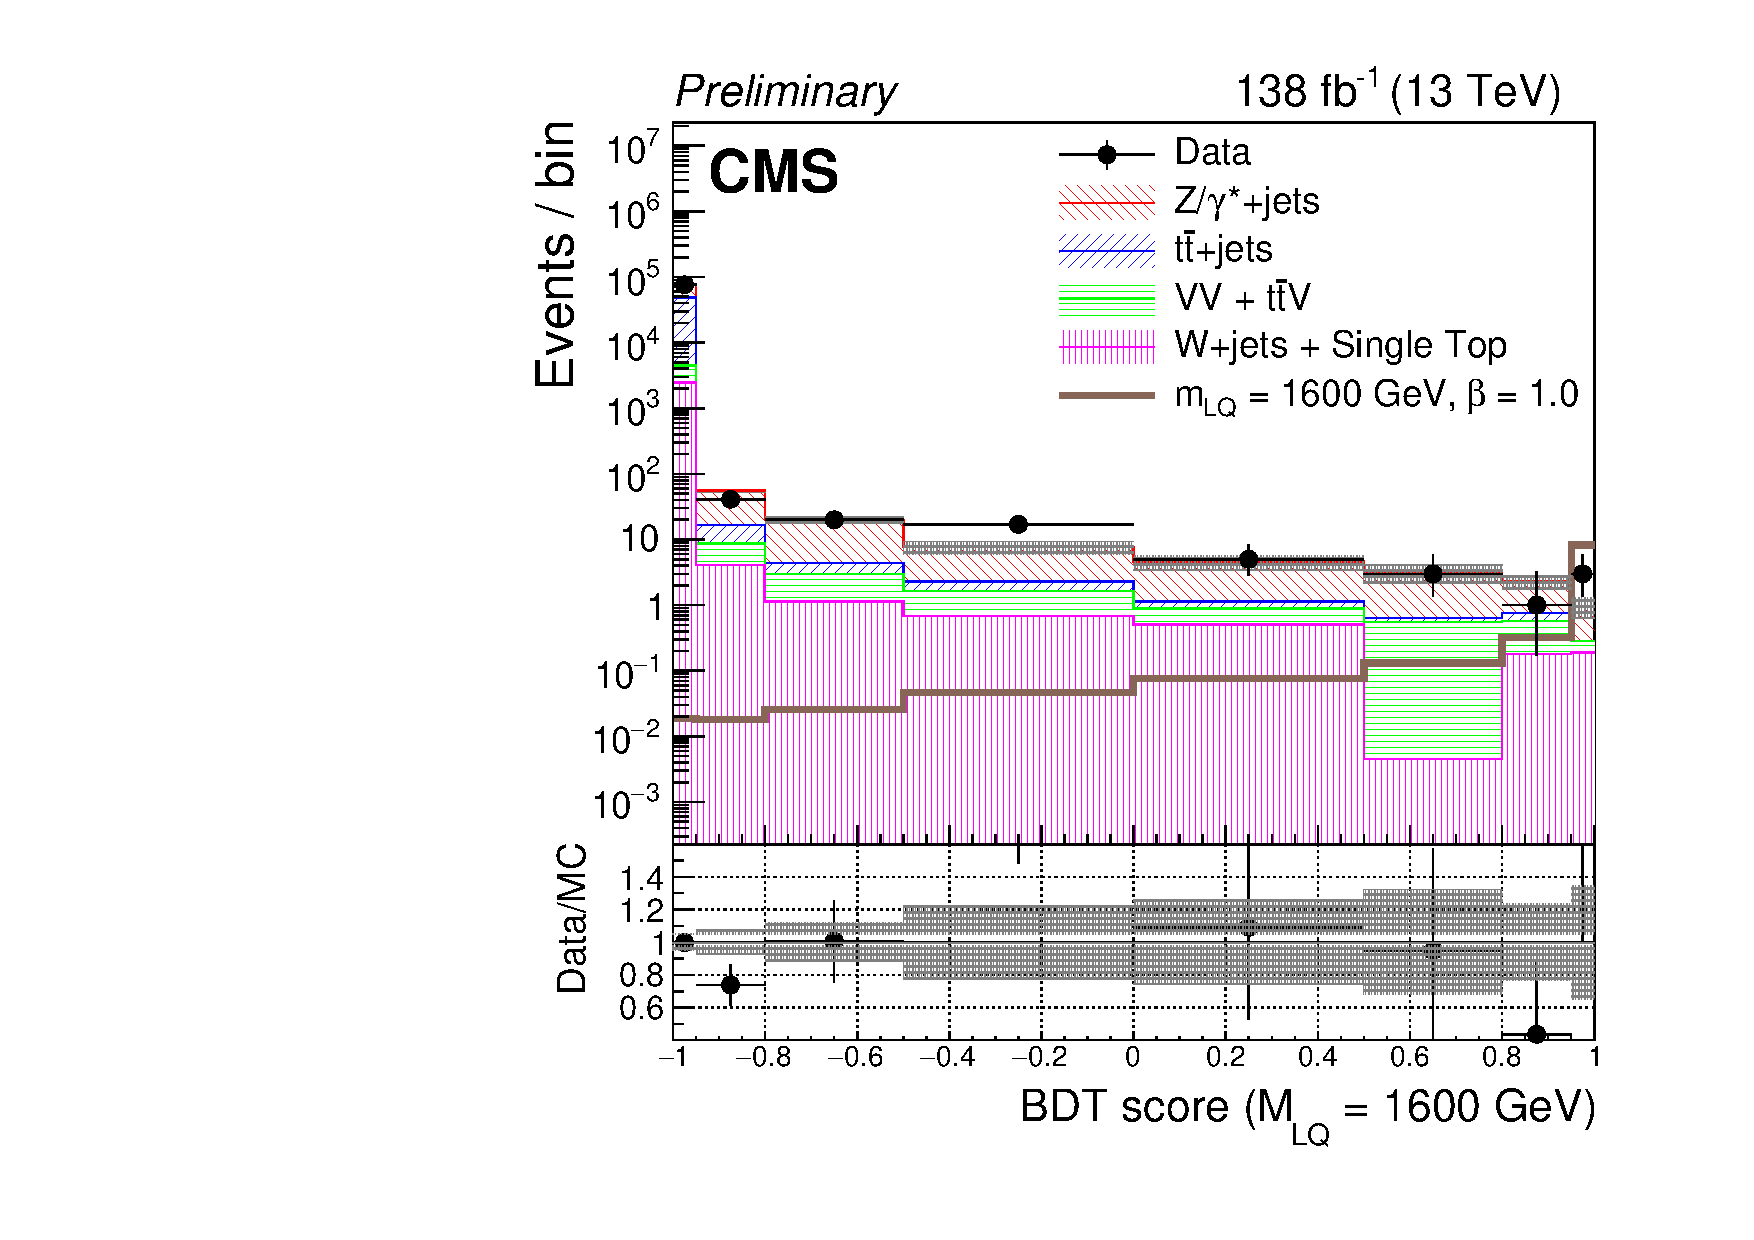
\includegraphics[width=.32\textwidth]{Images/Analysis/Results_combined_Unblinded/Plots/Preselection/BasicLQ_uujj_LQToBMu_pair_uubj_BDT_discrim_M1600_standard.pdf}}
    {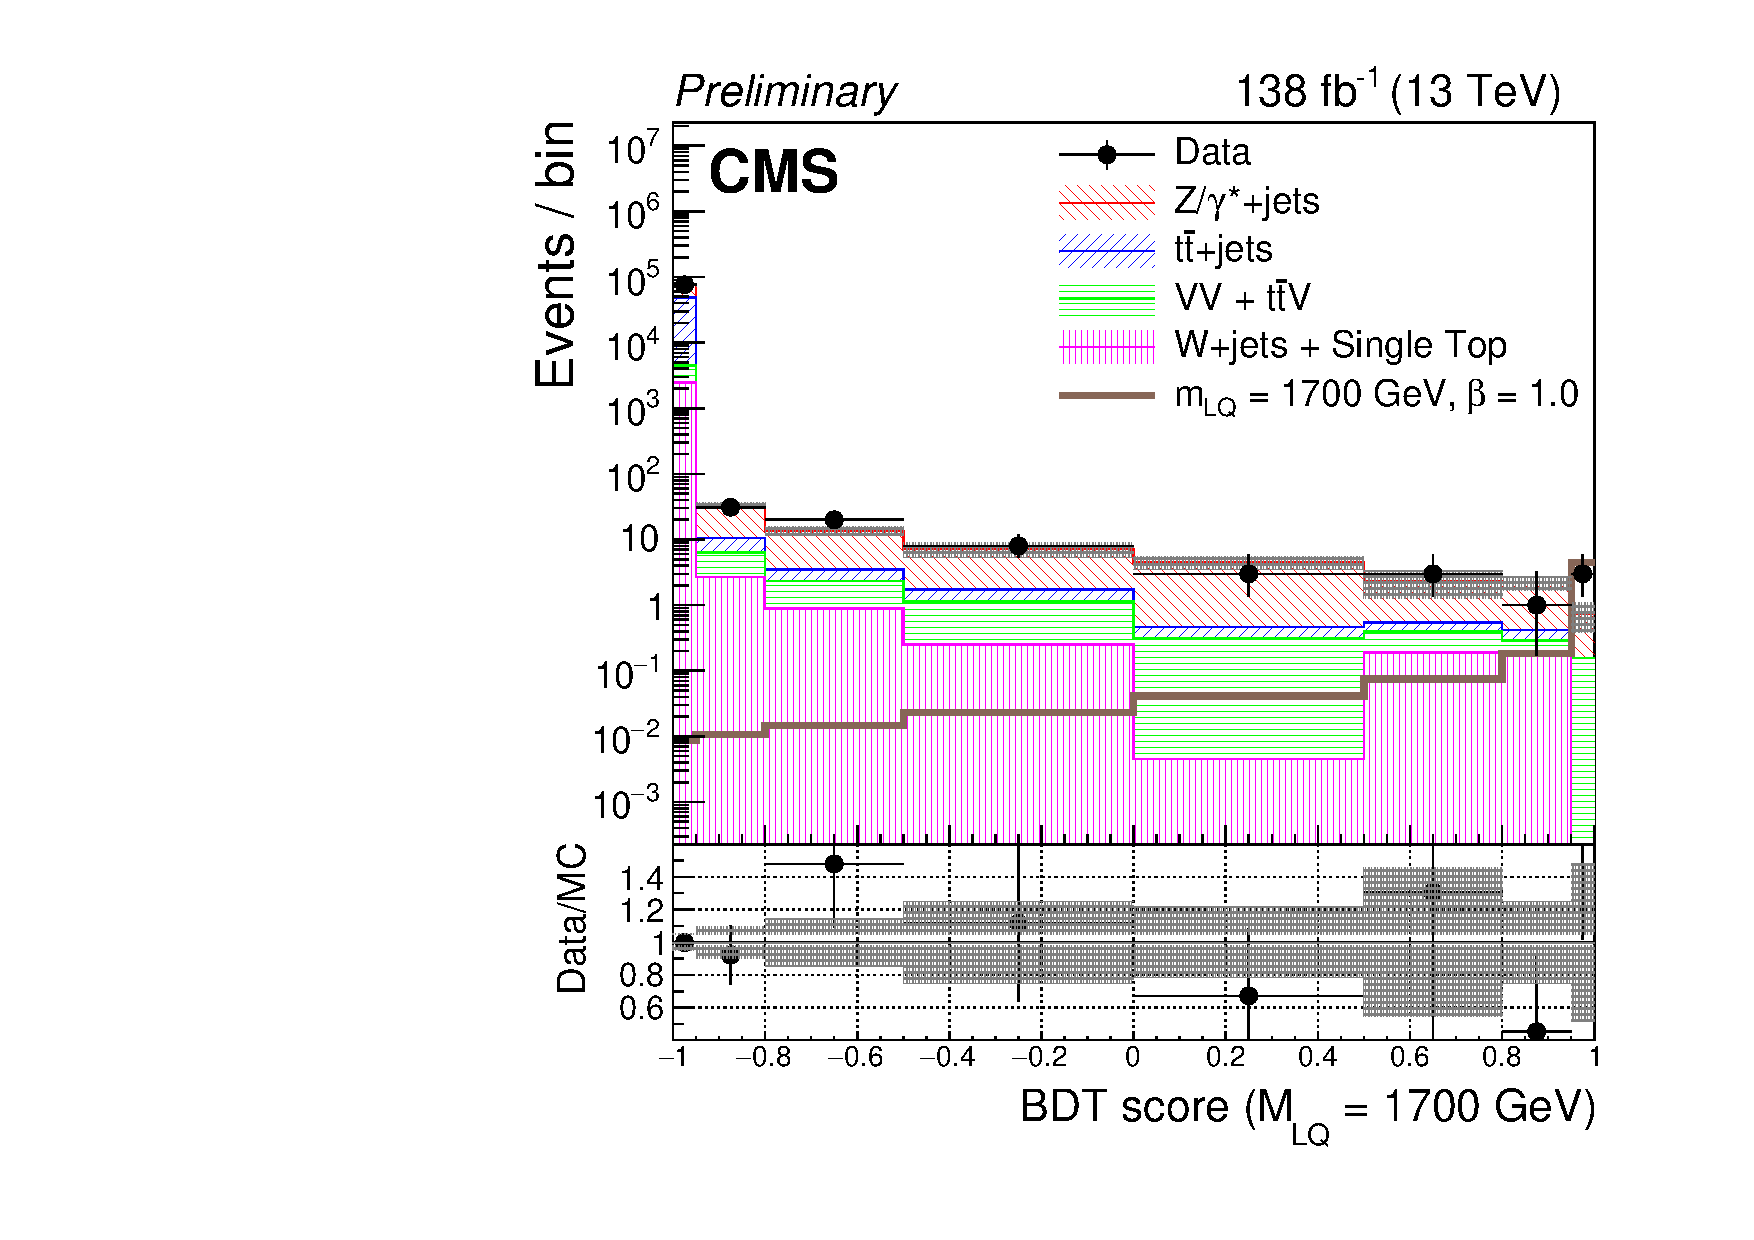
\includegraphics[width=.32\textwidth]{Images/Analysis/Results_combined_Unblinded/Plots/Preselection/BasicLQ_uujj_LQToBMu_pair_uubj_BDT_discrim_M1700_standard.pdf}}
    {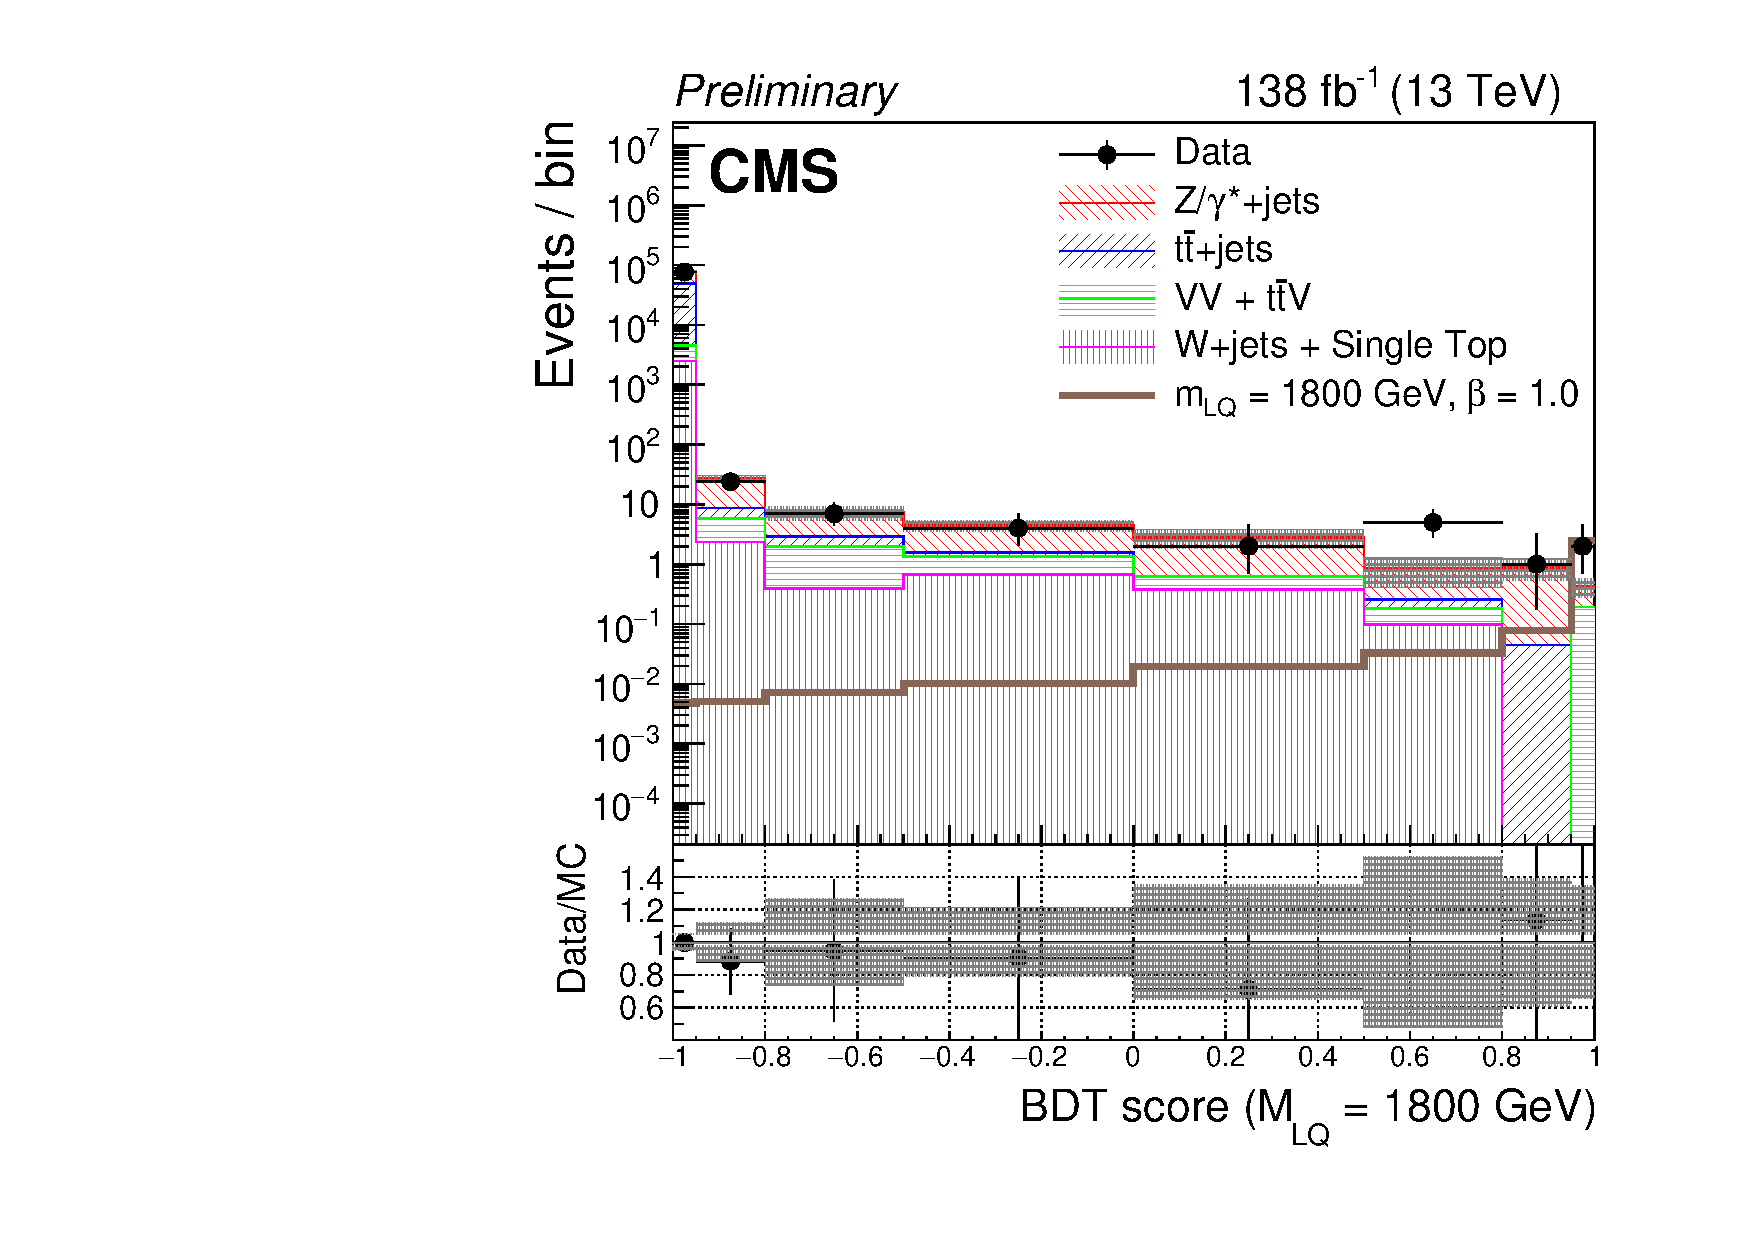
\includegraphics[width=.32\textwidth]{Images/Analysis/Results_combined_Unblinded/Plots/Preselection/BasicLQ_uujj_LQToBMu_pair_uubj_BDT_discrim_M1800_standard.pdf}}
    {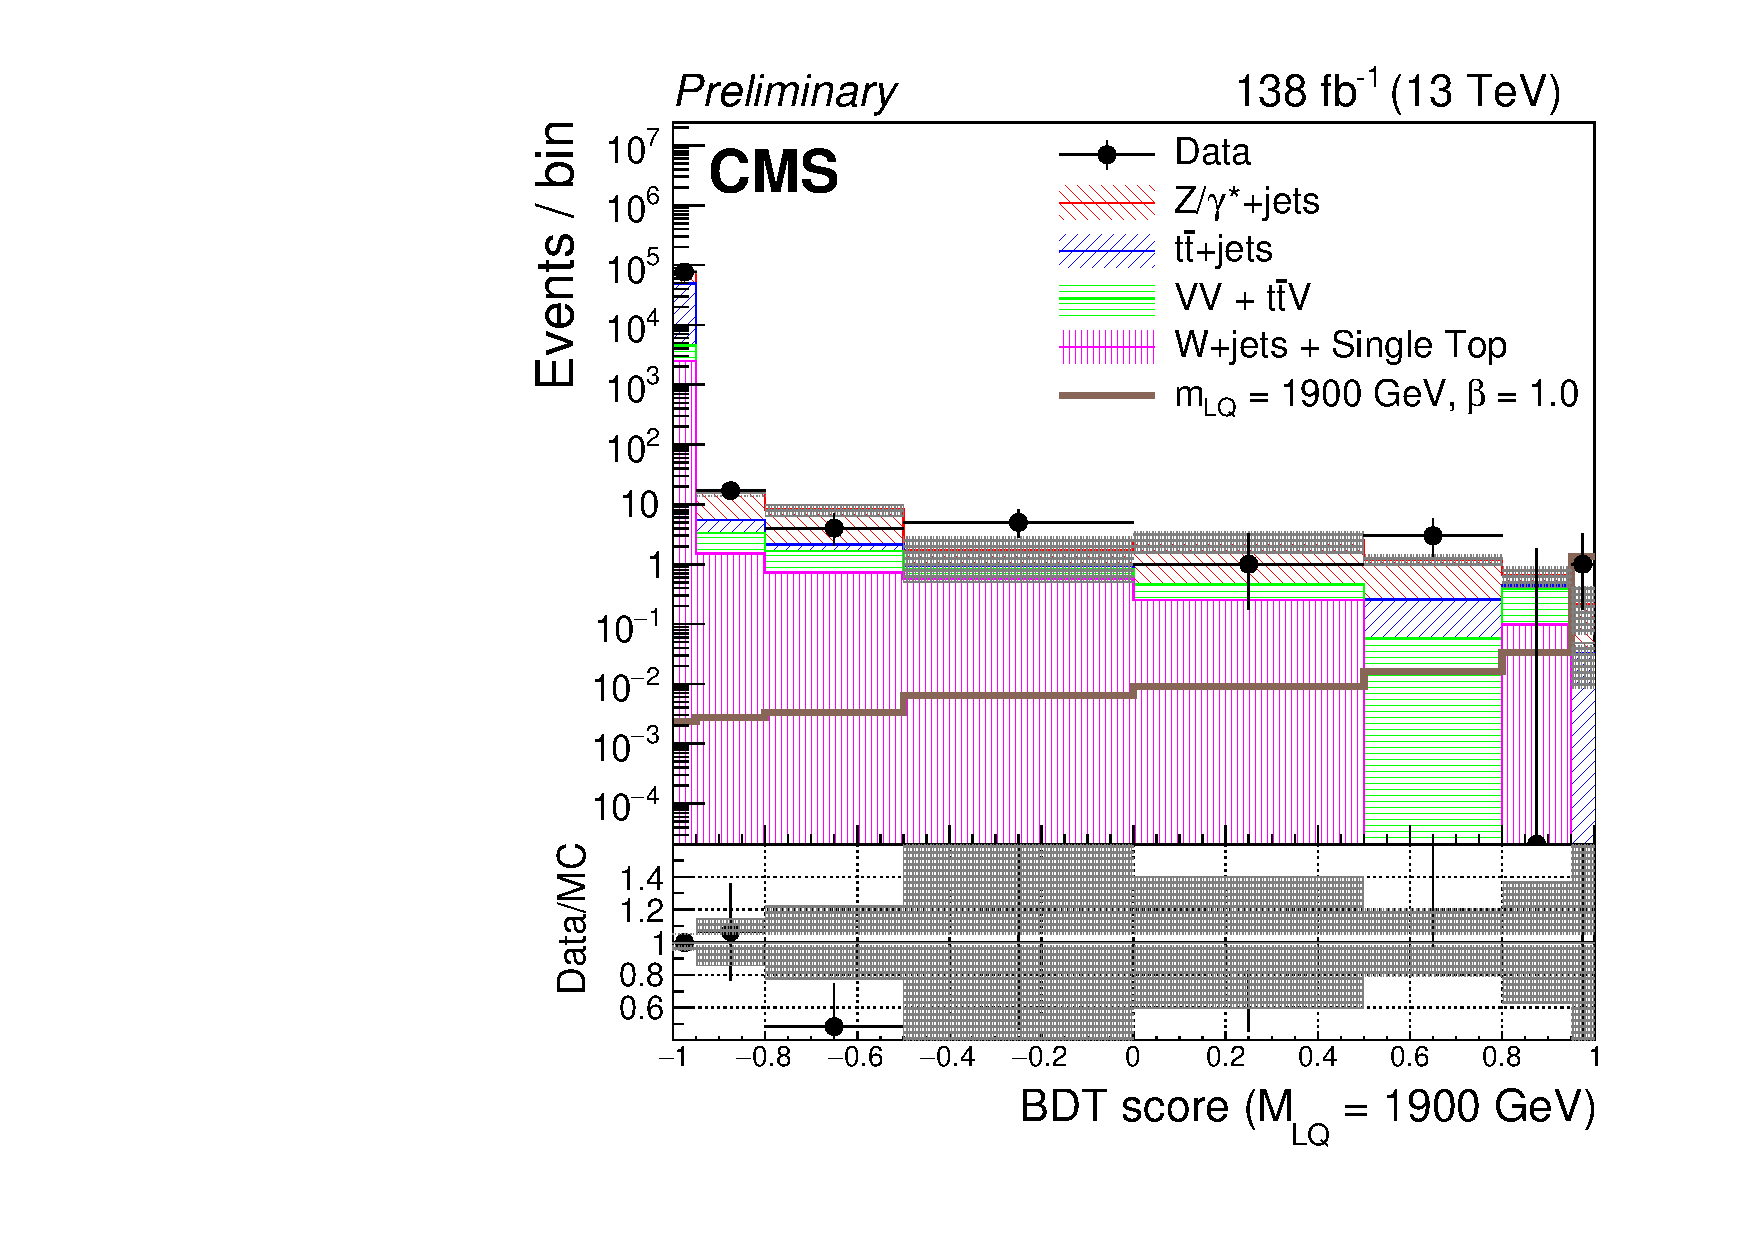
\includegraphics[width=.32\textwidth]{Images/Analysis/Results_combined_Unblinded/Plots/Preselection/BasicLQ_uujj_LQToBMu_pair_uubj_BDT_discrim_M1900_standard.pdf}}
    {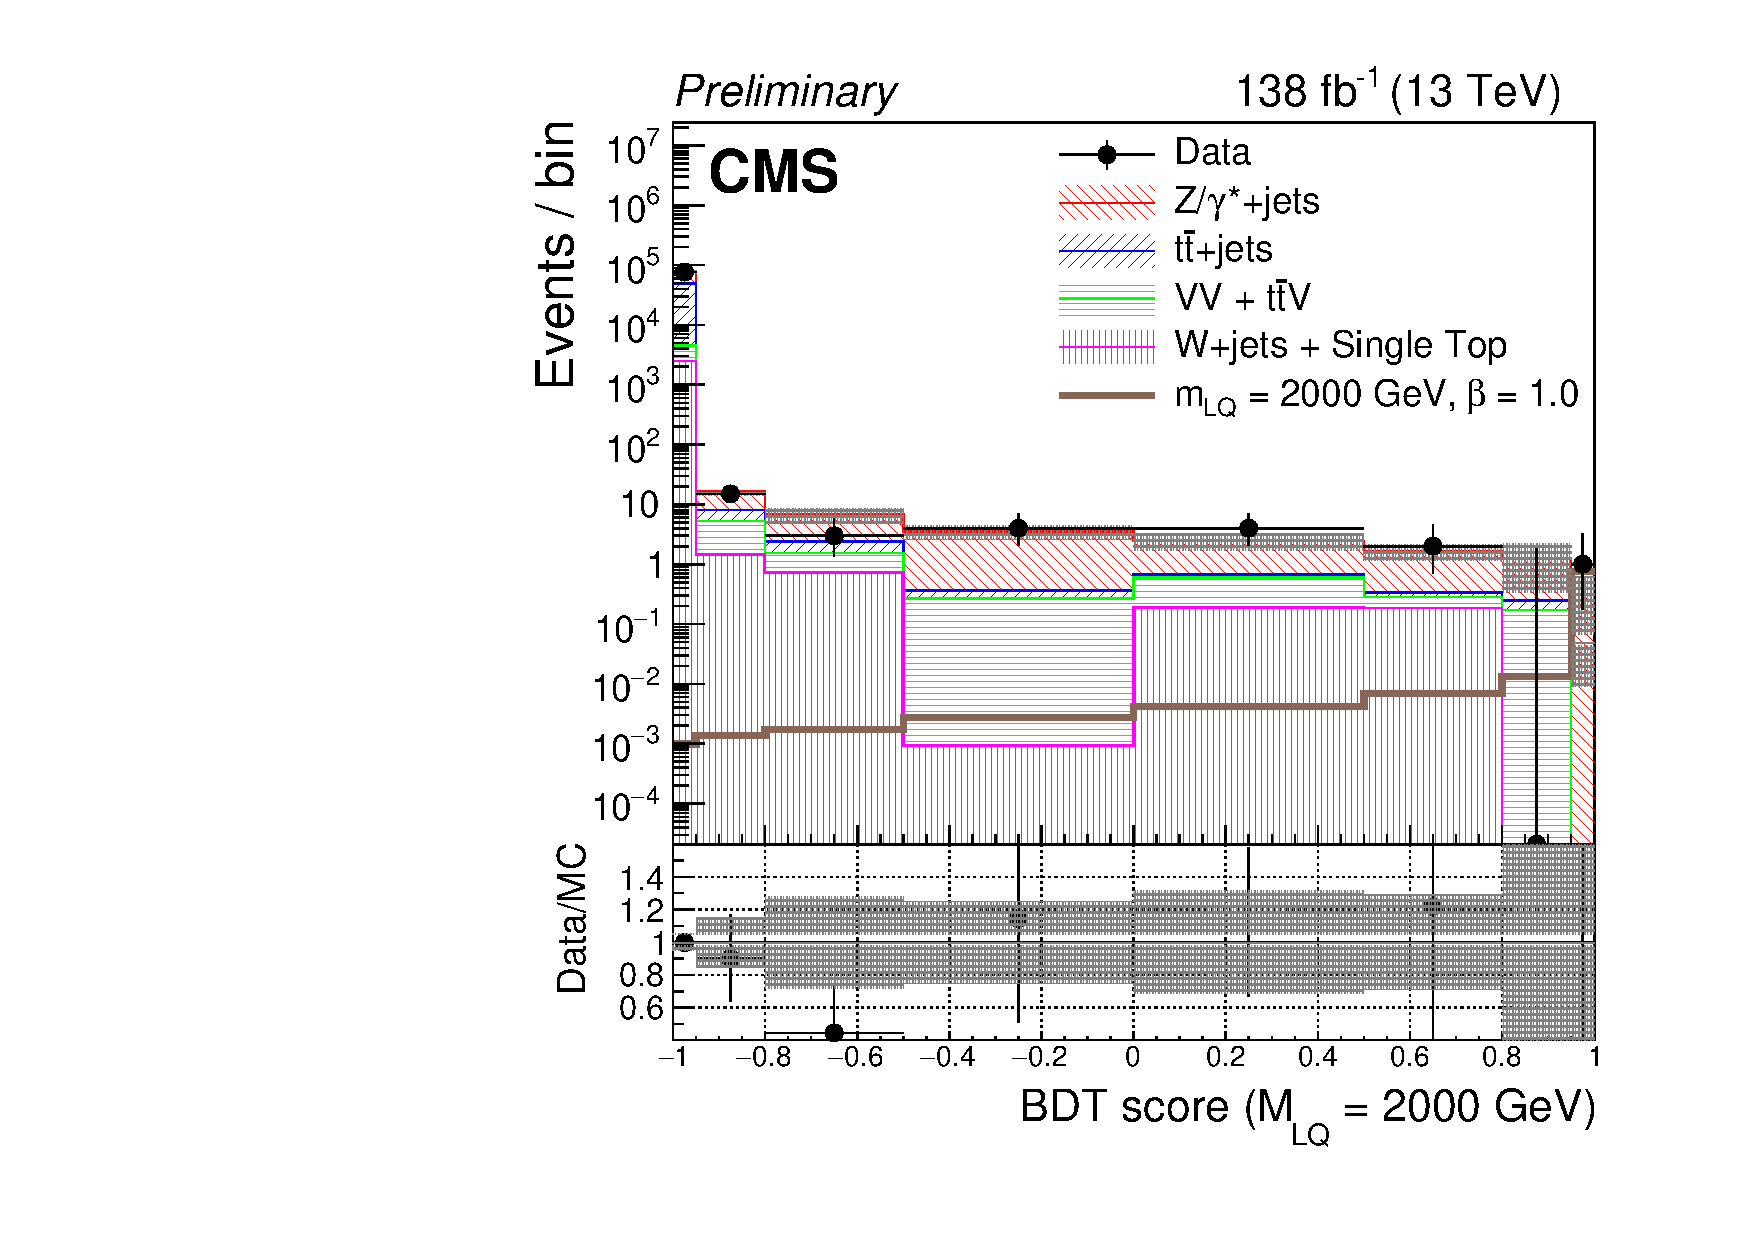
\includegraphics[width=.32\textwidth]{Images/Analysis/Results_combined_Unblinded/Plots/Preselection/BasicLQ_uujj_LQToBMu_pair_uubj_BDT_discrim_M2000_standard.pdf}}
    {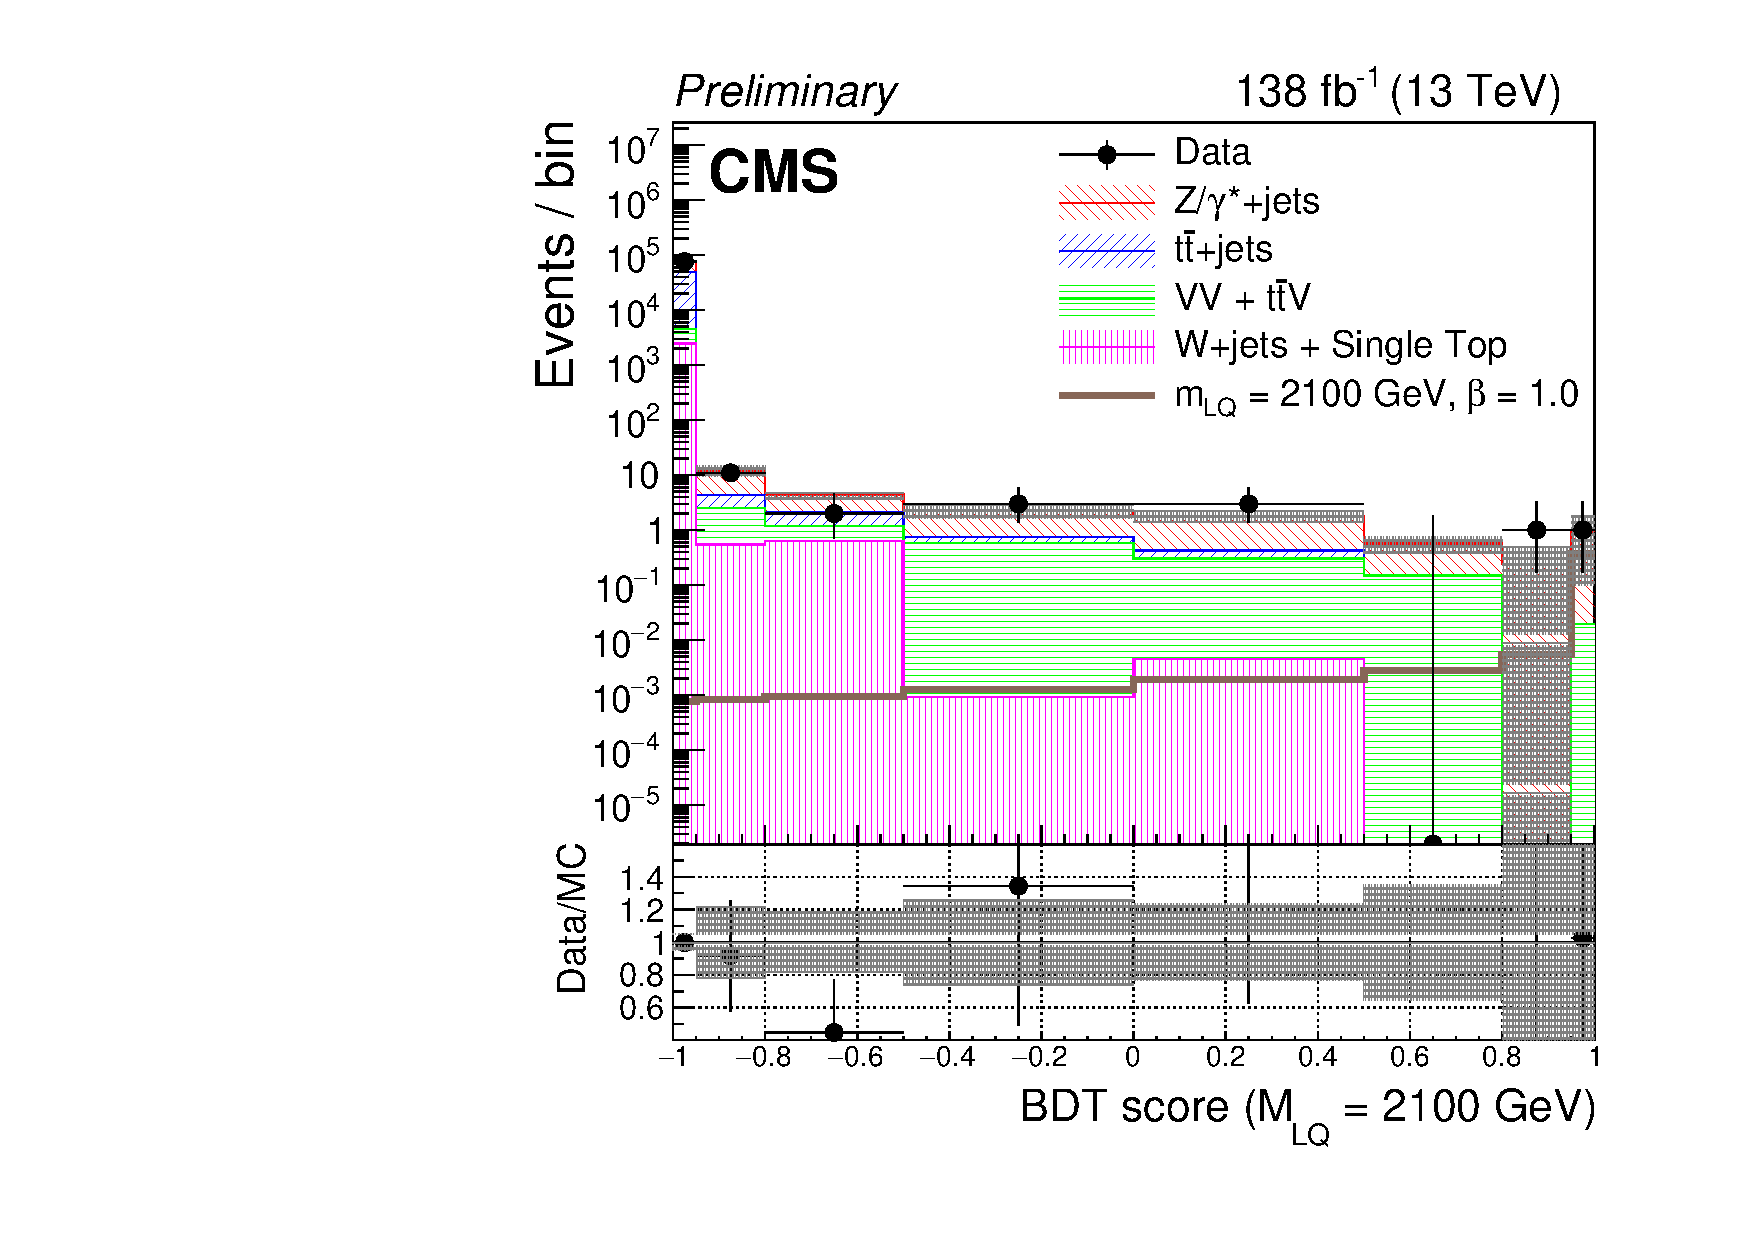
\includegraphics[width=.32\textwidth]{Images/Analysis/Results_combined_Unblinded/Plots/Preselection/BasicLQ_uujj_LQToBMu_pair_uubj_BDT_discrim_M2100_standard.pdf}}
    {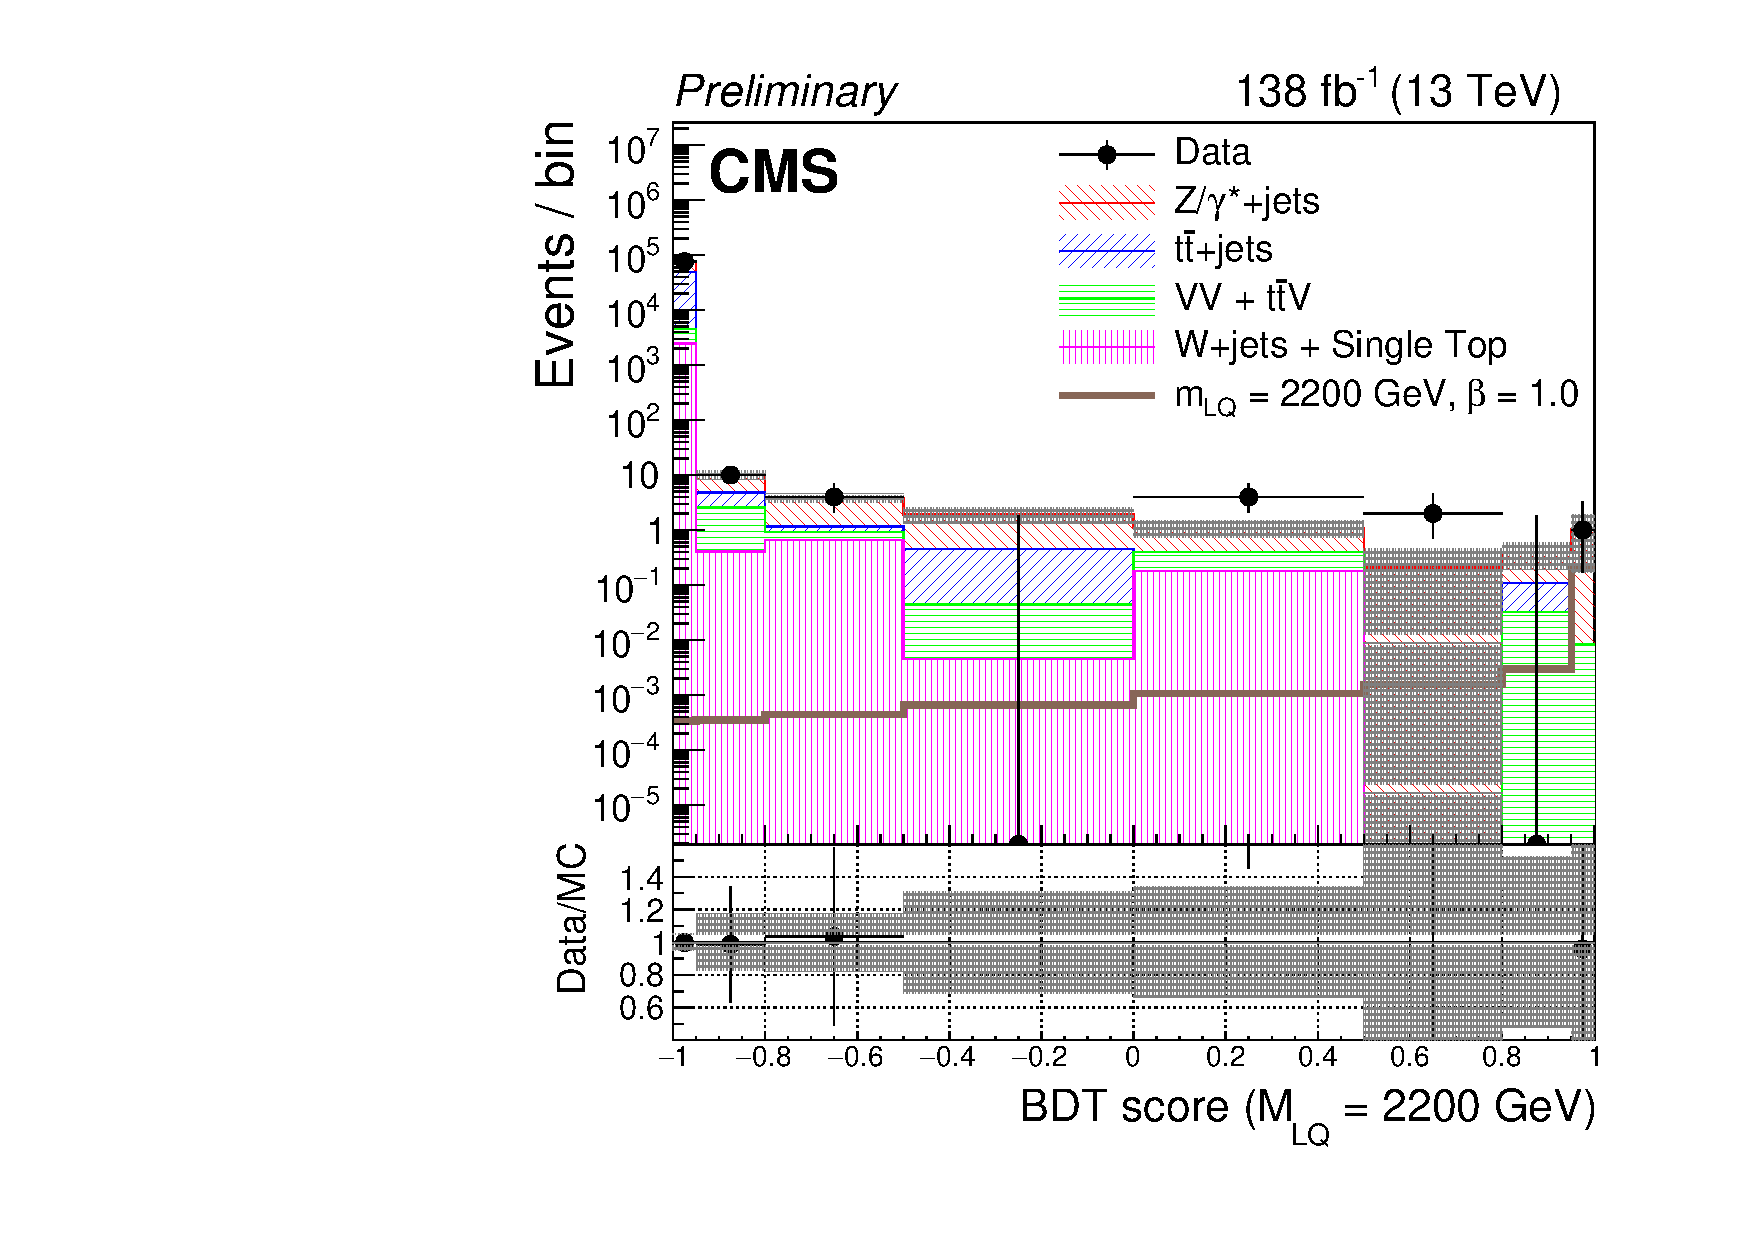
\includegraphics[width=.32\textwidth]{Images/Analysis/Results_combined_Unblinded/Plots/Preselection/BasicLQ_uujj_LQToBMu_pair_uubj_BDT_discrim_M2200_standard.pdf}}
    {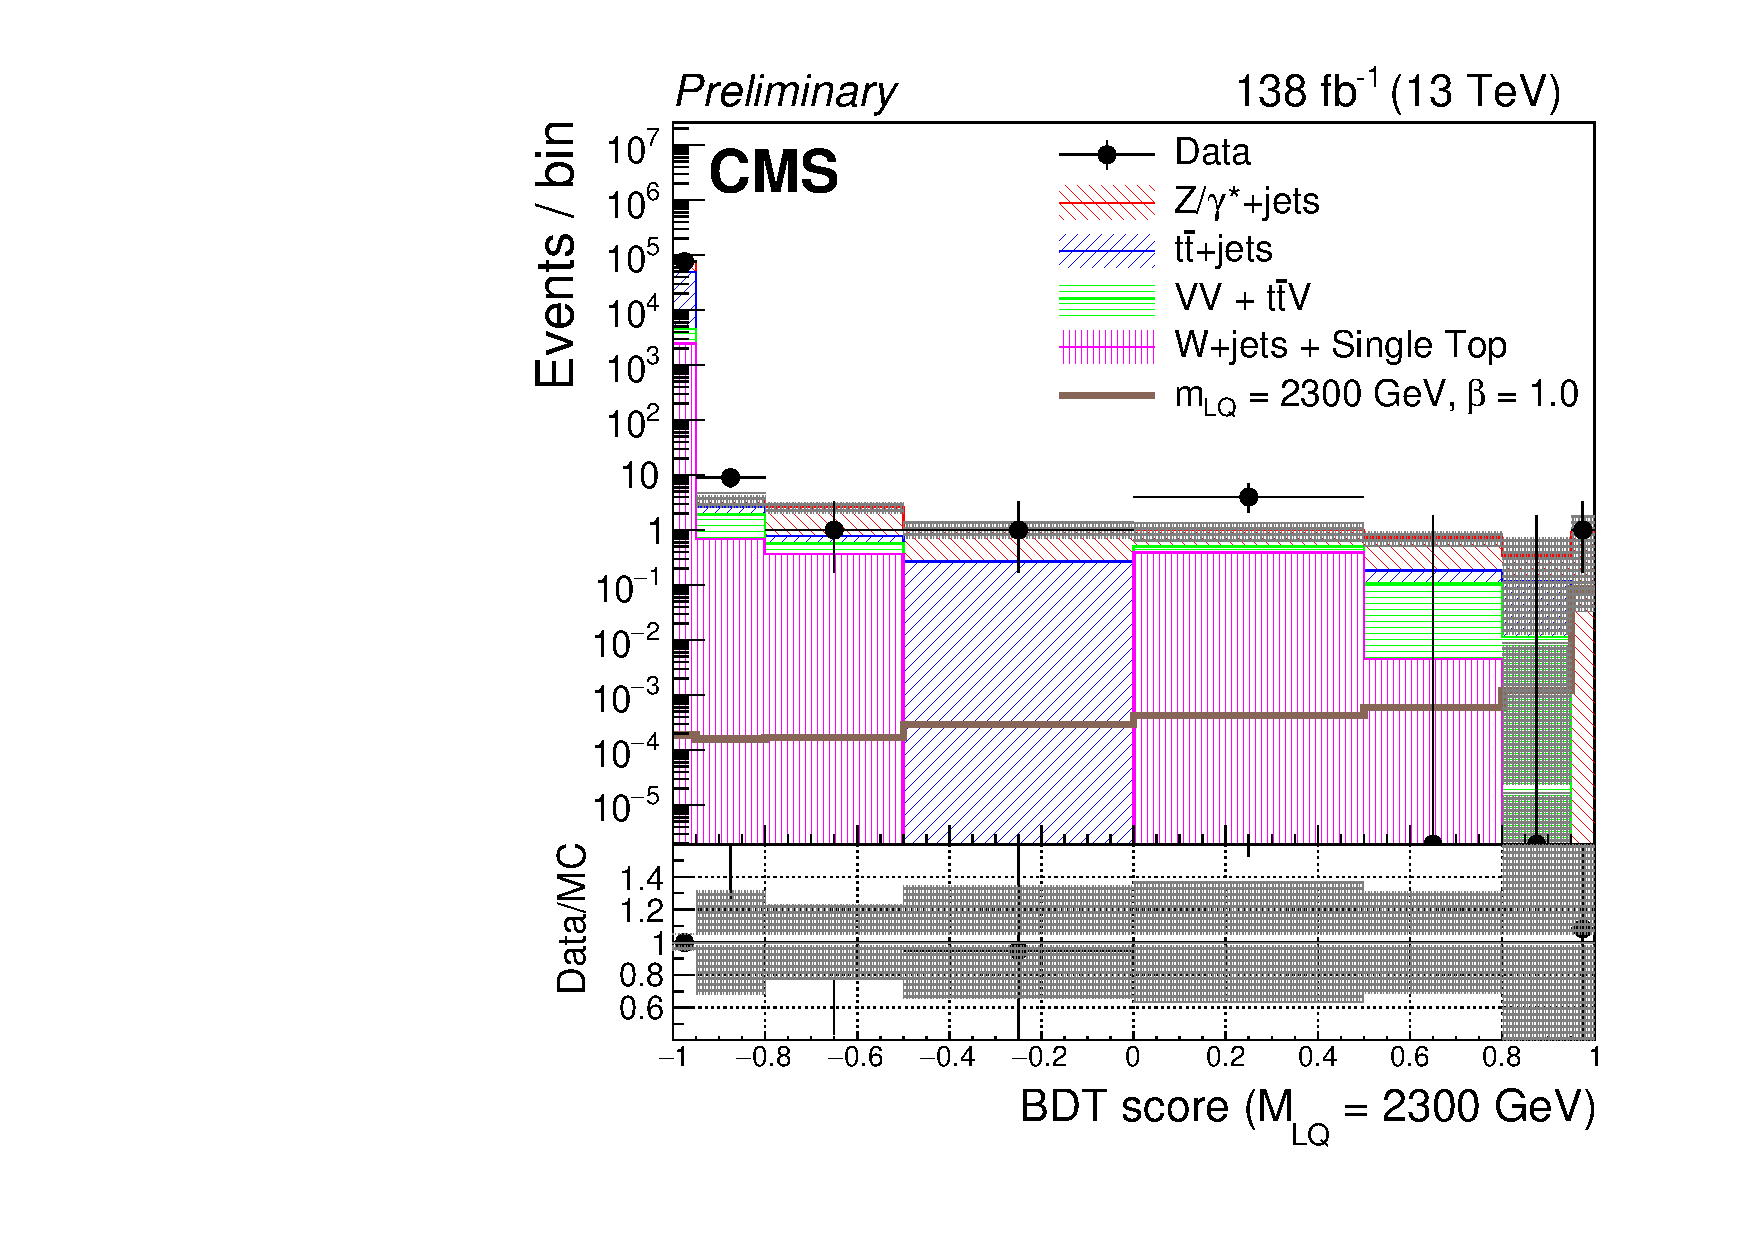
\includegraphics[width=.32\textwidth]{Images/Analysis/Results_combined_Unblinded/Plots/Preselection/BasicLQ_uujj_LQToBMu_pair_uubj_BDT_discrim_M2300_standard.pdf}}
    {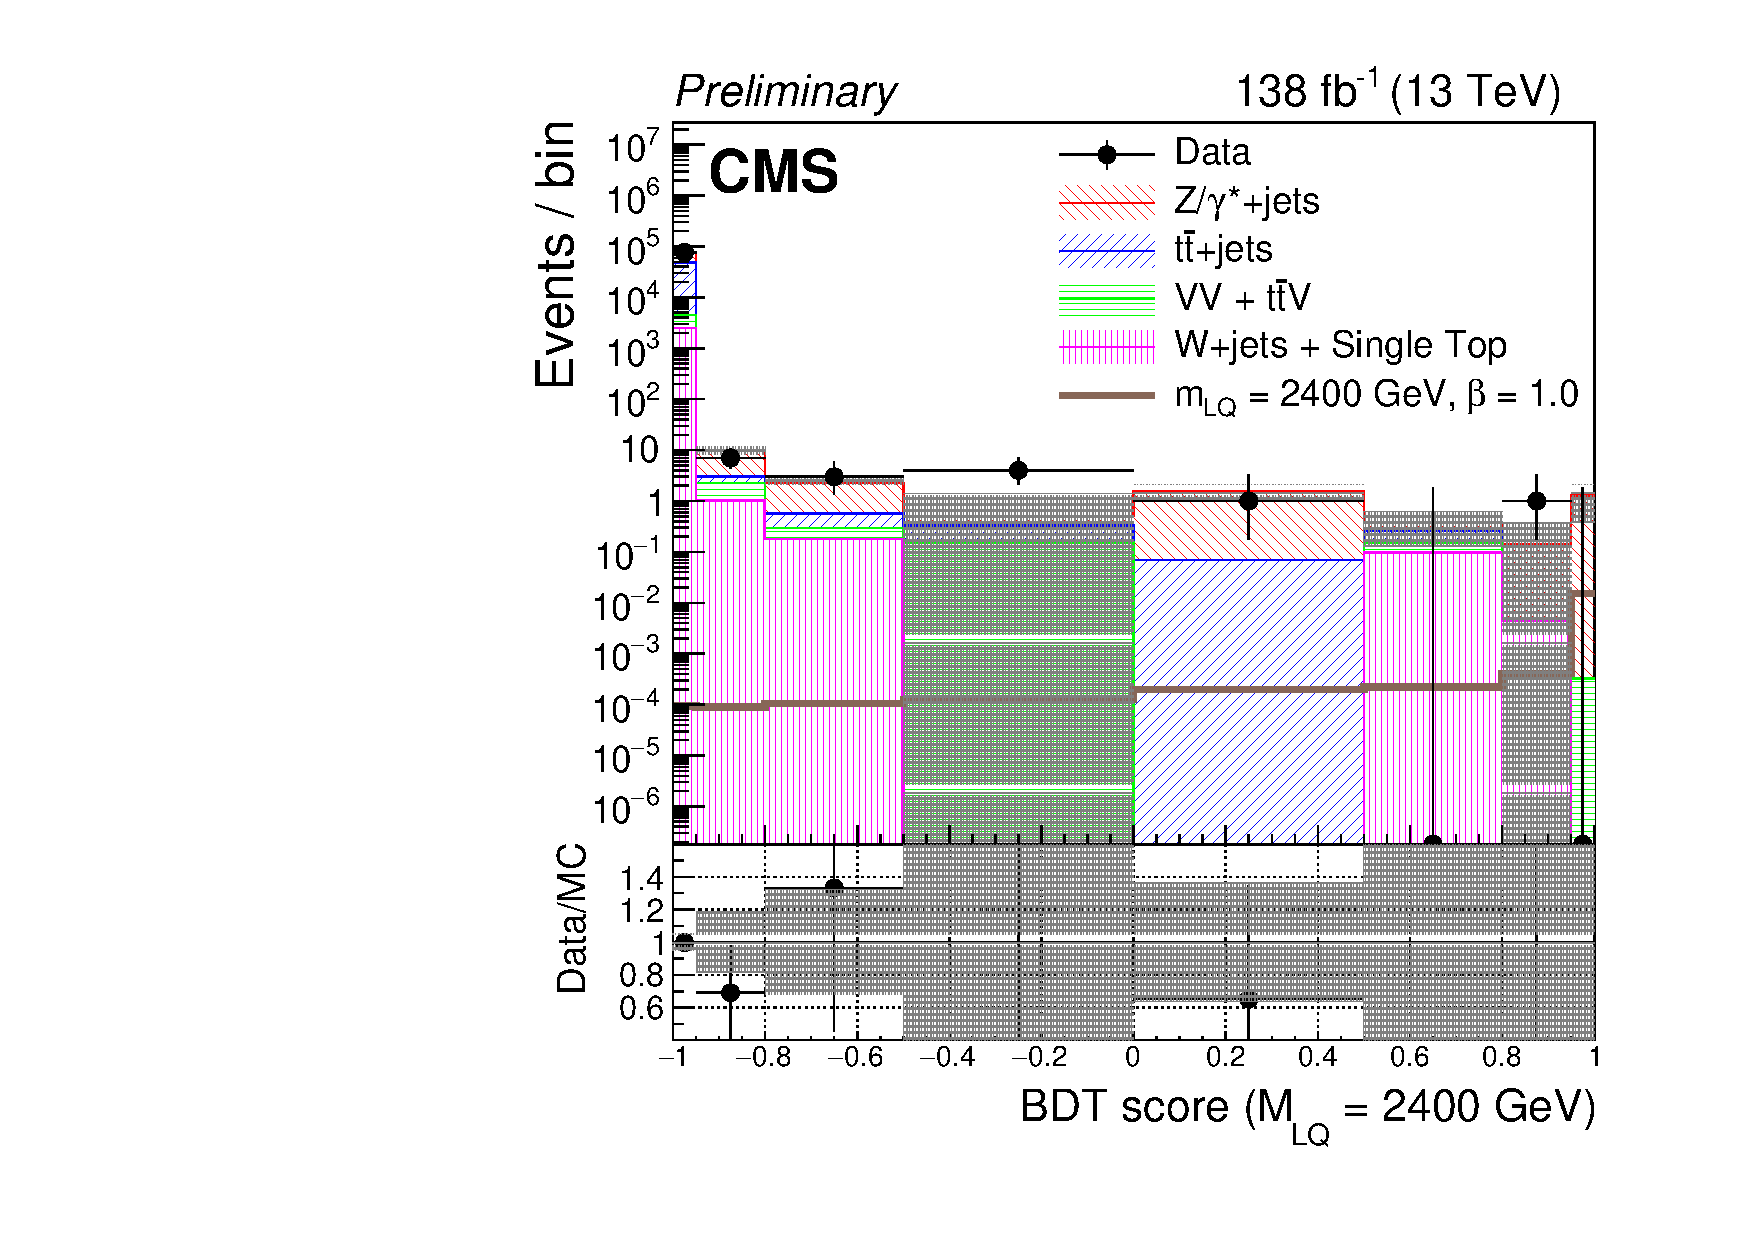
\includegraphics[width=.32\textwidth]{Images/Analysis/Results_combined_Unblinded/Plots/Preselection/BasicLQ_uujj_LQToBMu_pair_uubj_BDT_discrim_M2400_standard.pdf}}
    {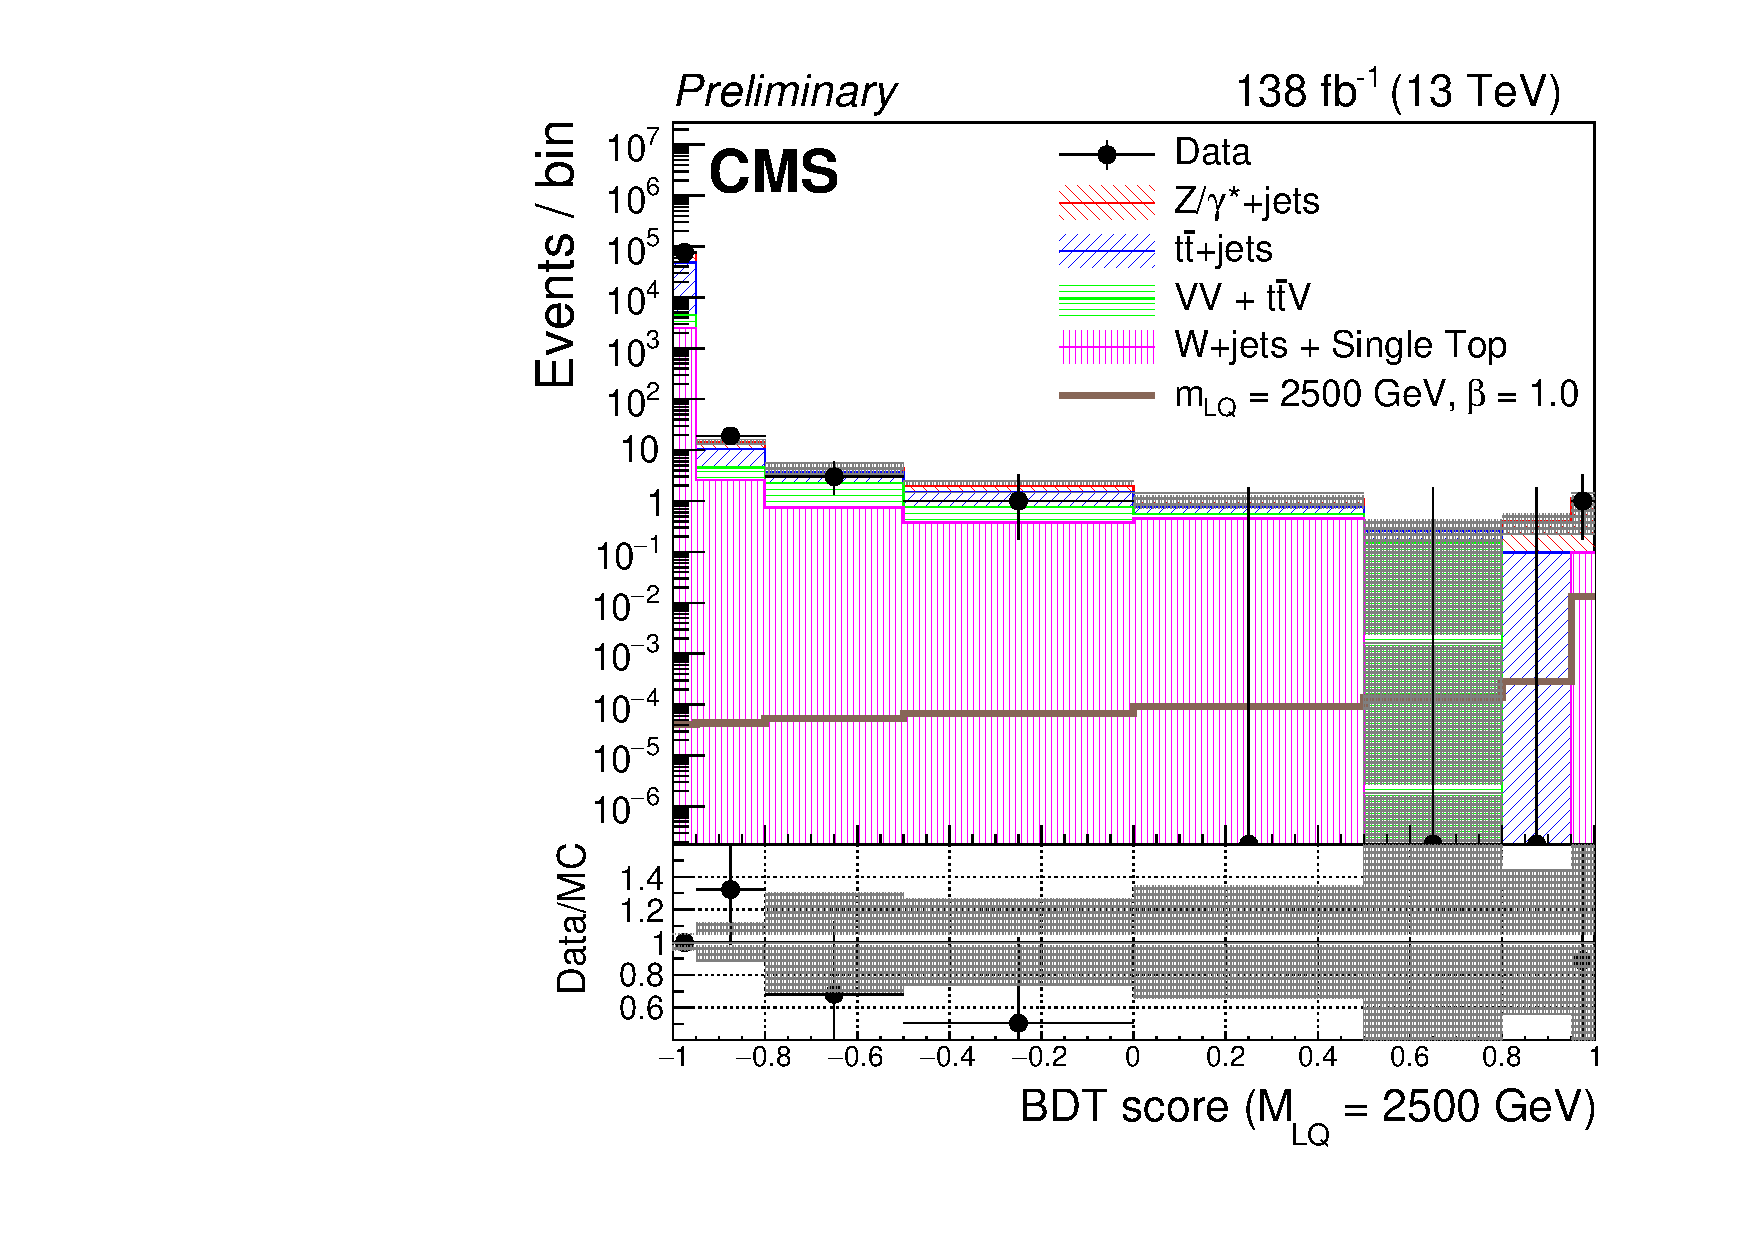
\includegraphics[width=.32\textwidth]{Images/Analysis/Results_combined_Unblinded/Plots/Preselection/BasicLQ_uujj_LQToBMu_pair_uubj_BDT_discrim_M2500_standard.pdf}}
    {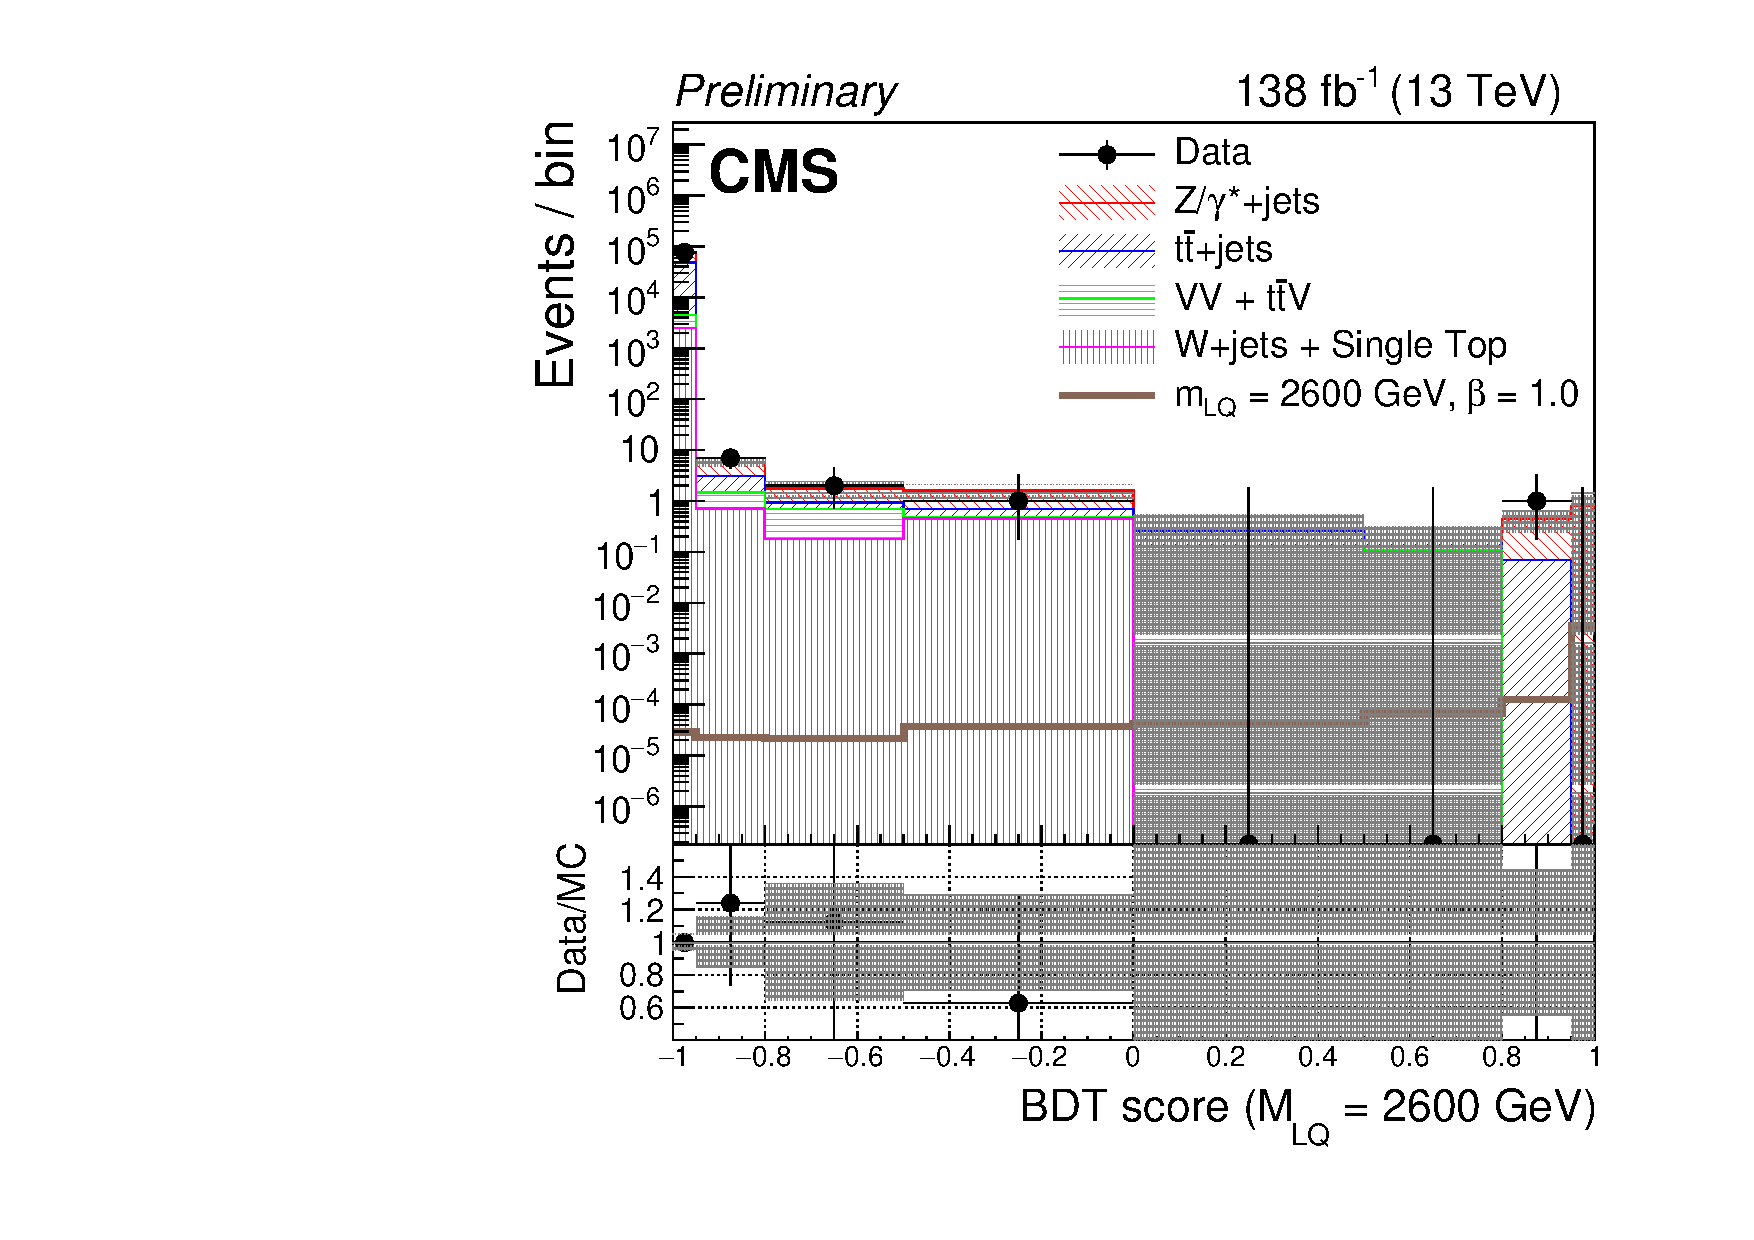
\includegraphics[width=.32\textwidth]{Images/Analysis/Results_combined_Unblinded/Plots/Preselection/BasicLQ_uujj_LQToBMu_pair_uubj_BDT_discrim_M2600_standard.pdf}}

    \caption{A comparison between observed and expected events of BDT responses at preselection level in the combination of 2016, 2017, and 2018 data. The leptoquark mass of the signal in each plot corresponds to the leptoquark mass used in the BDT training. Error bars represent statistical uncertainties, while the shaded area represents systematic uncertainties.
    \label{figapp:BDT1500to2600}}
\end{figure}

\begin{figure}[H]
    \centering
    {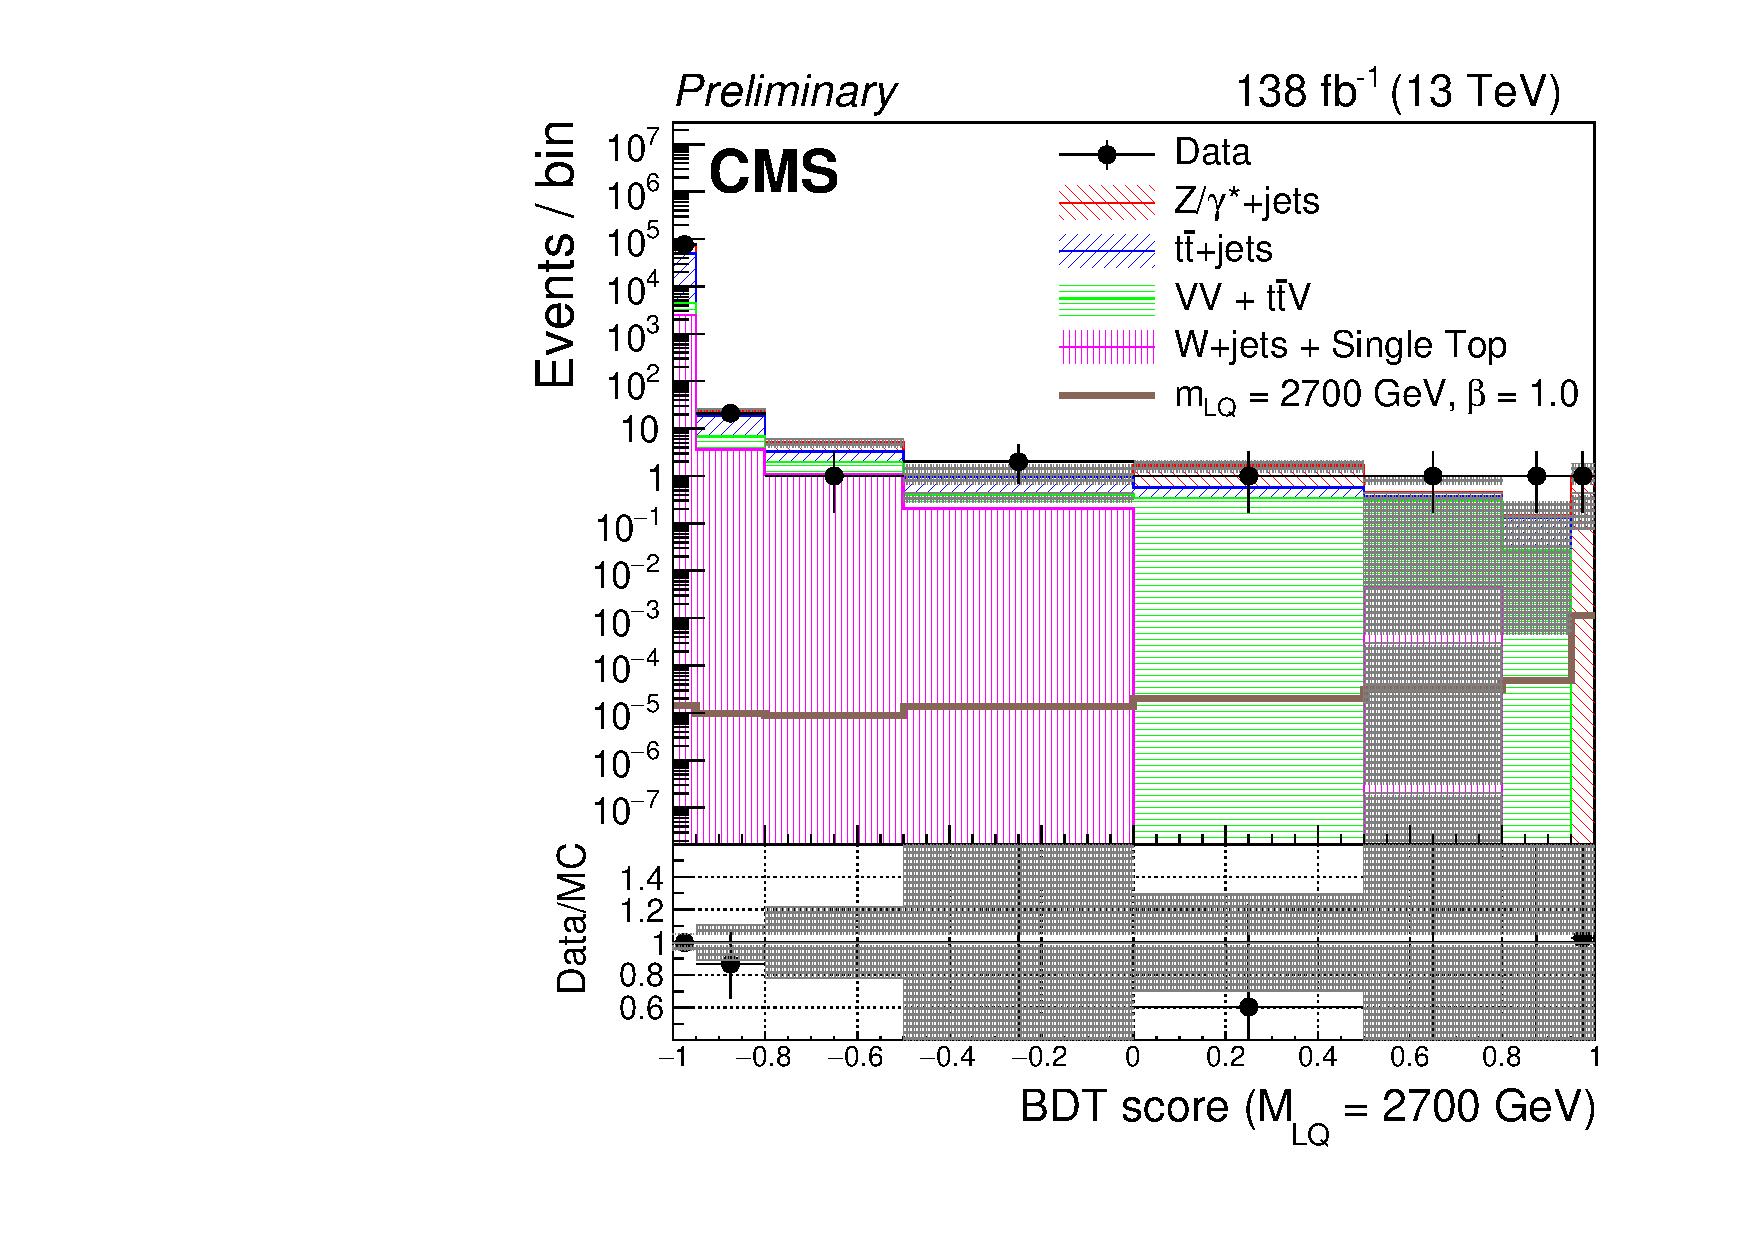
\includegraphics[width=.32\textwidth]{Images/Analysis/Results_combined_Unblinded/Plots/Preselection/BasicLQ_uujj_LQToBMu_pair_uubj_BDT_discrim_M2700_standard.pdf}}
    {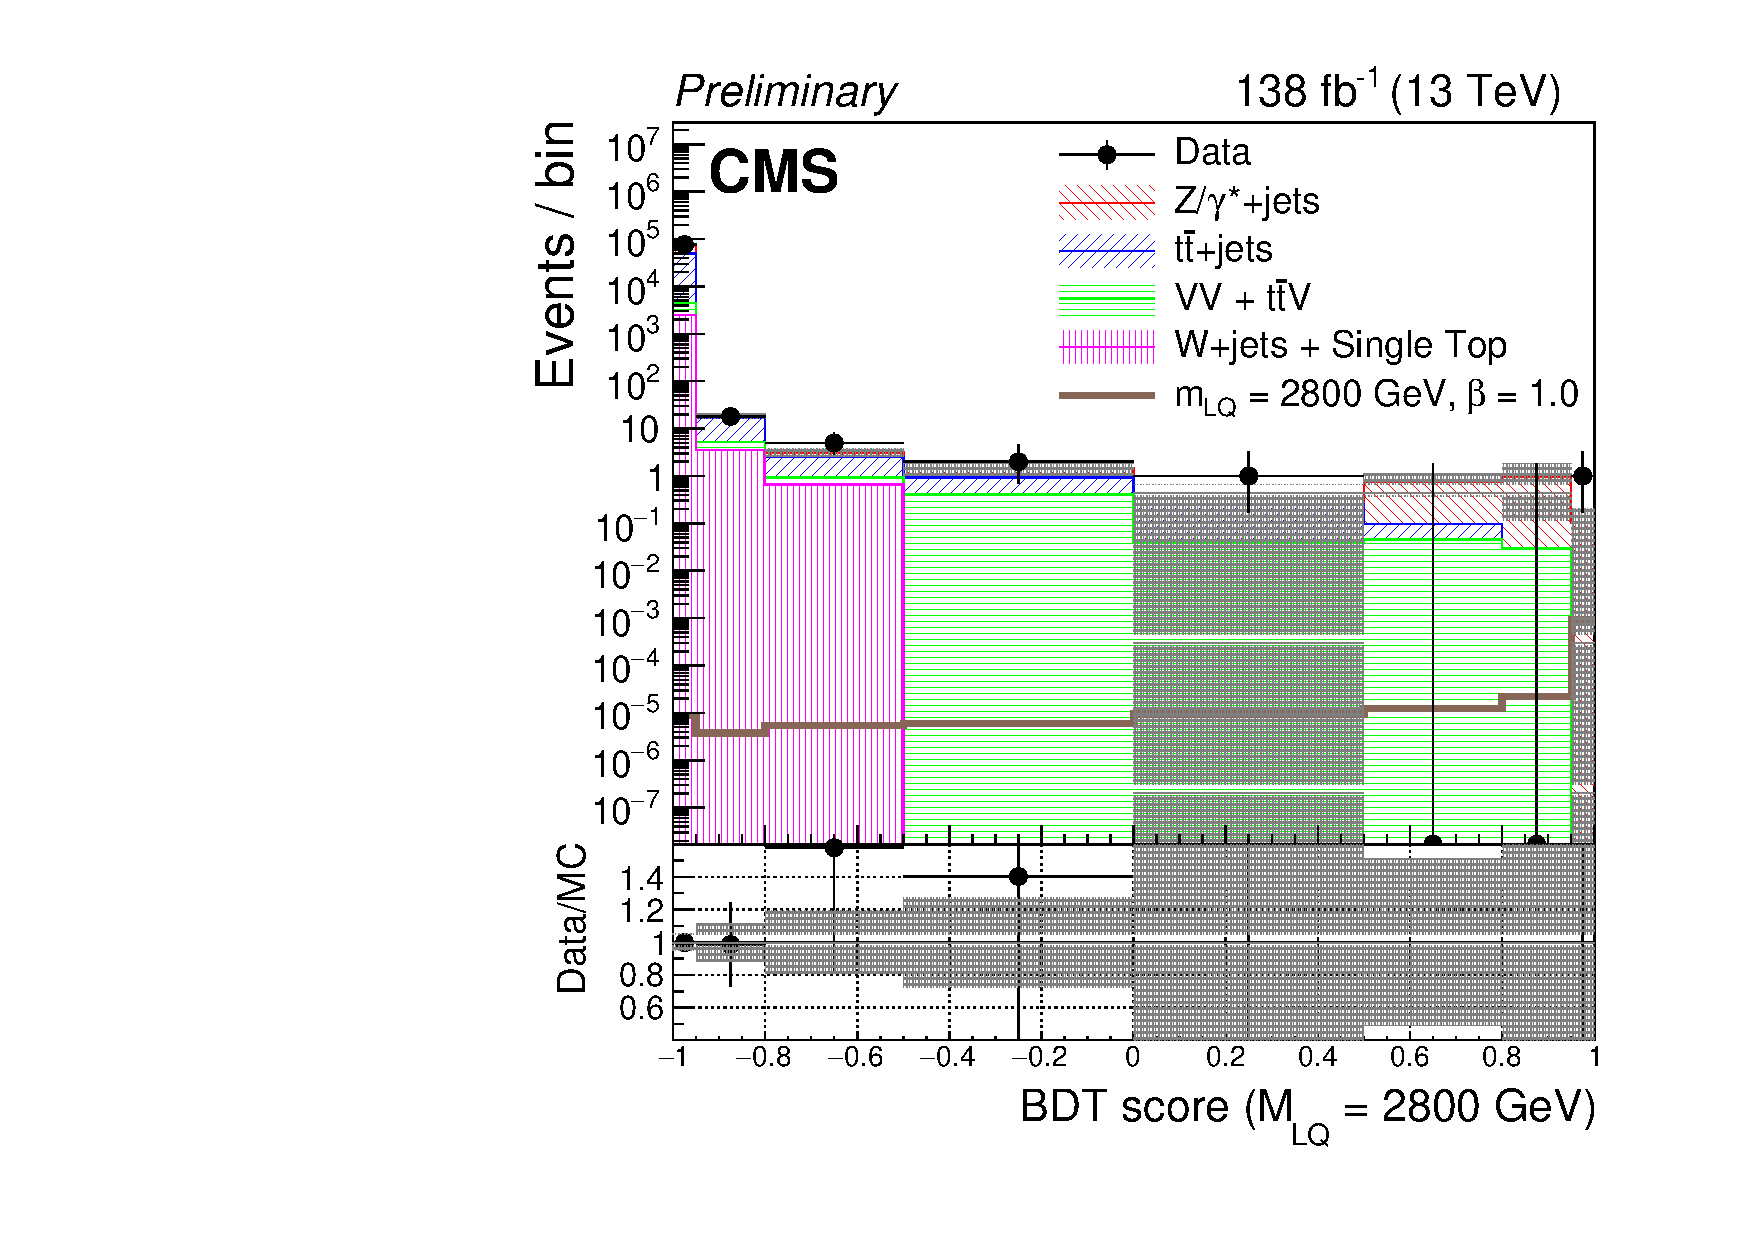
\includegraphics[width=.32\textwidth]{Images/Analysis/Results_combined_Unblinded/Plots/Preselection/BasicLQ_uujj_LQToBMu_pair_uubj_BDT_discrim_M2800_standard.pdf}}
    {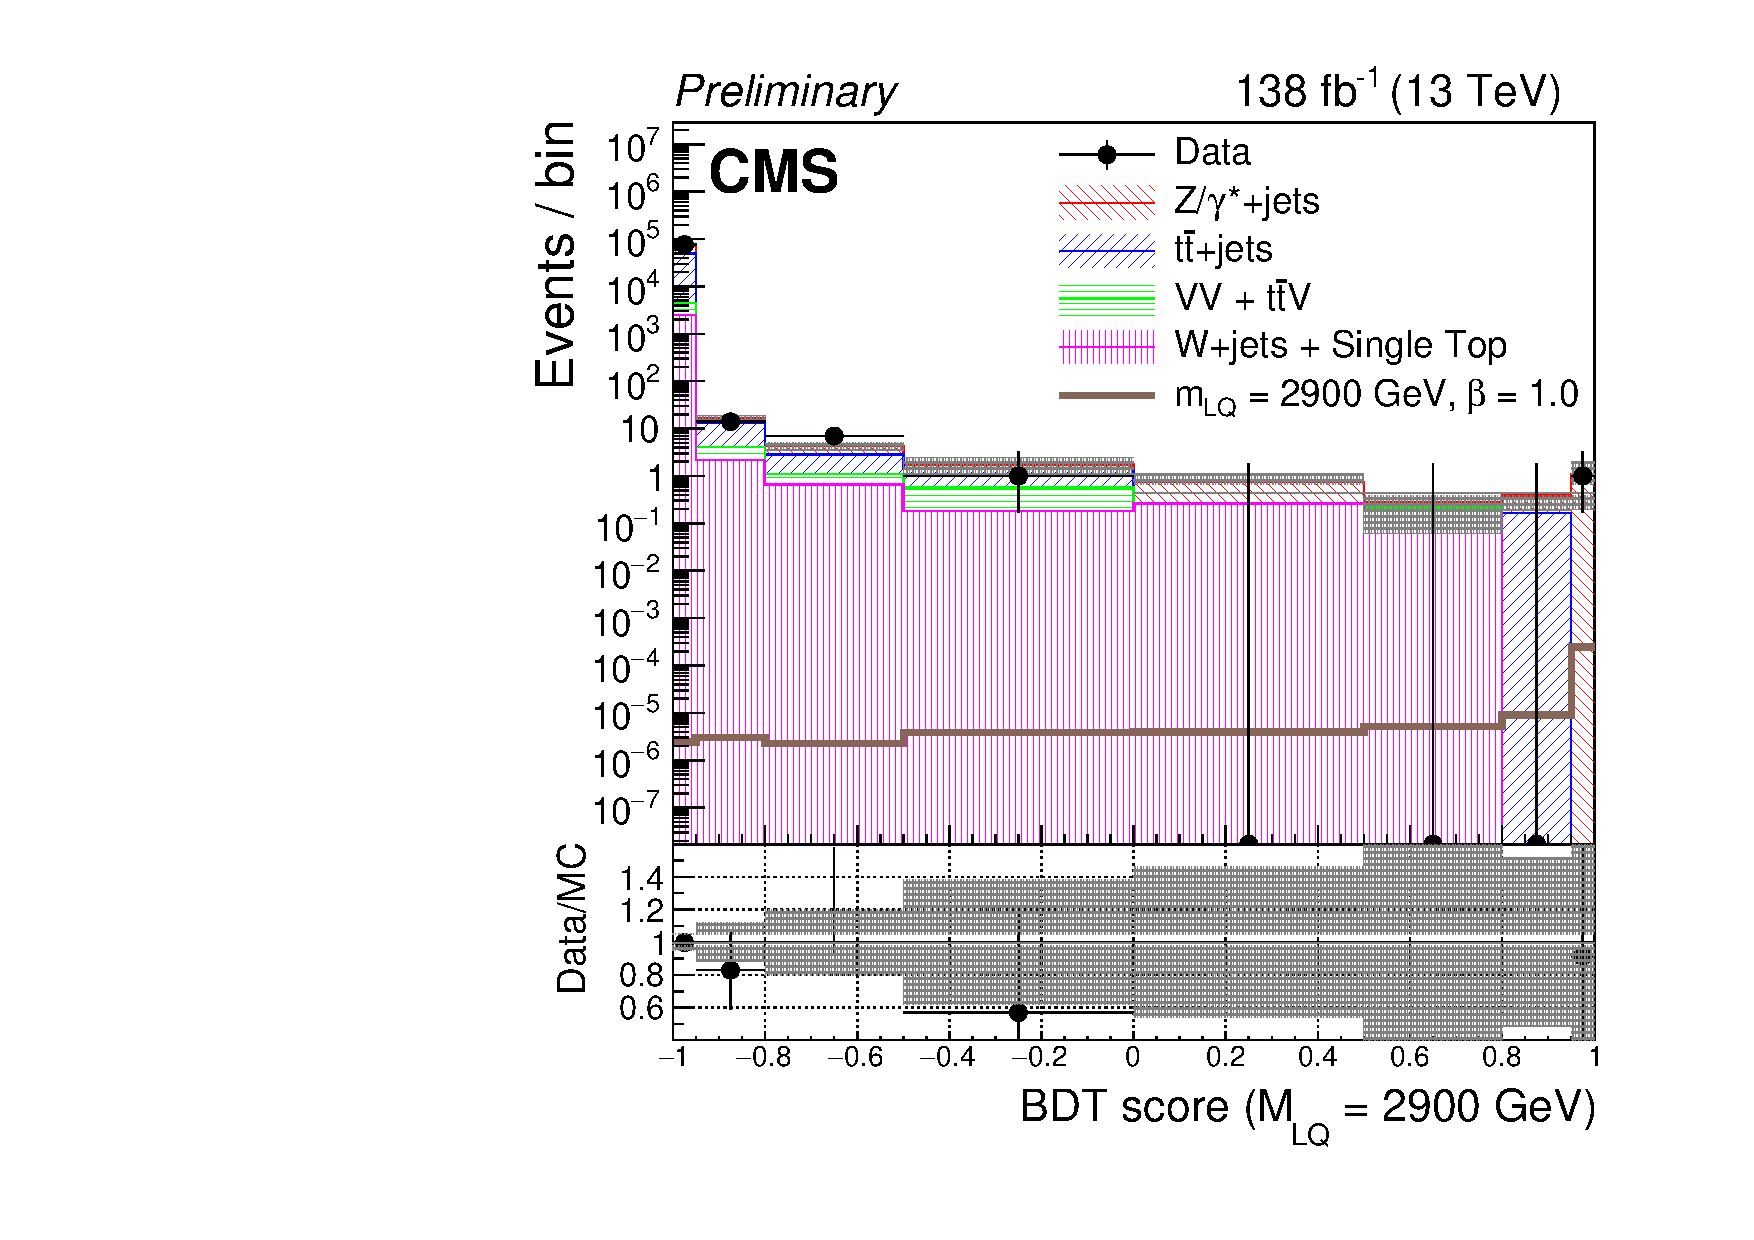
\includegraphics[width=.32\textwidth]{Images/Analysis/Results_combined_Unblinded/Plots/Preselection/BasicLQ_uujj_LQToBMu_pair_uubj_BDT_discrim_M2900_standard.pdf}}
    {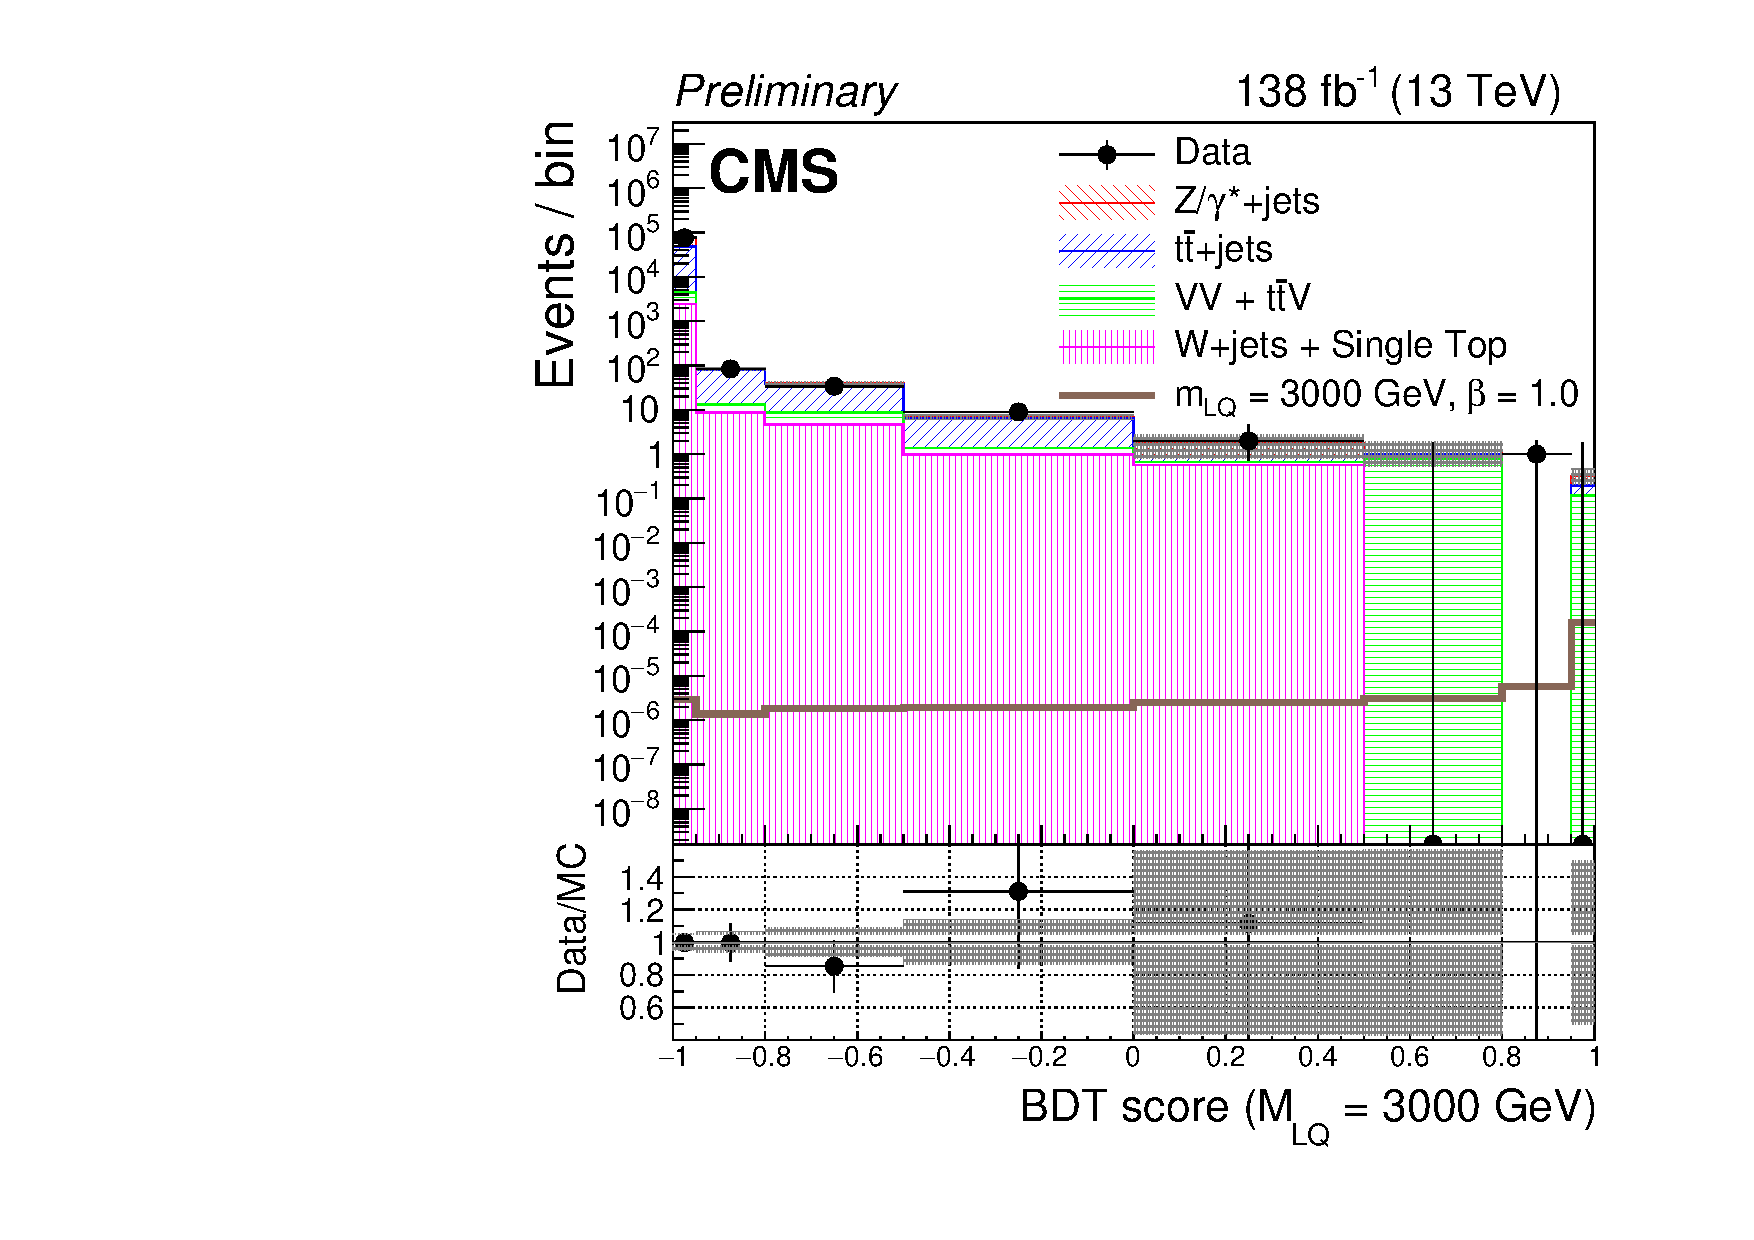
\includegraphics[width=.32\textwidth]{Images/Analysis/Results_combined_Unblinded/Plots/Preselection/BasicLQ_uujj_LQToBMu_pair_uubj_BDT_discrim_M3000_standard.pdf}}
    {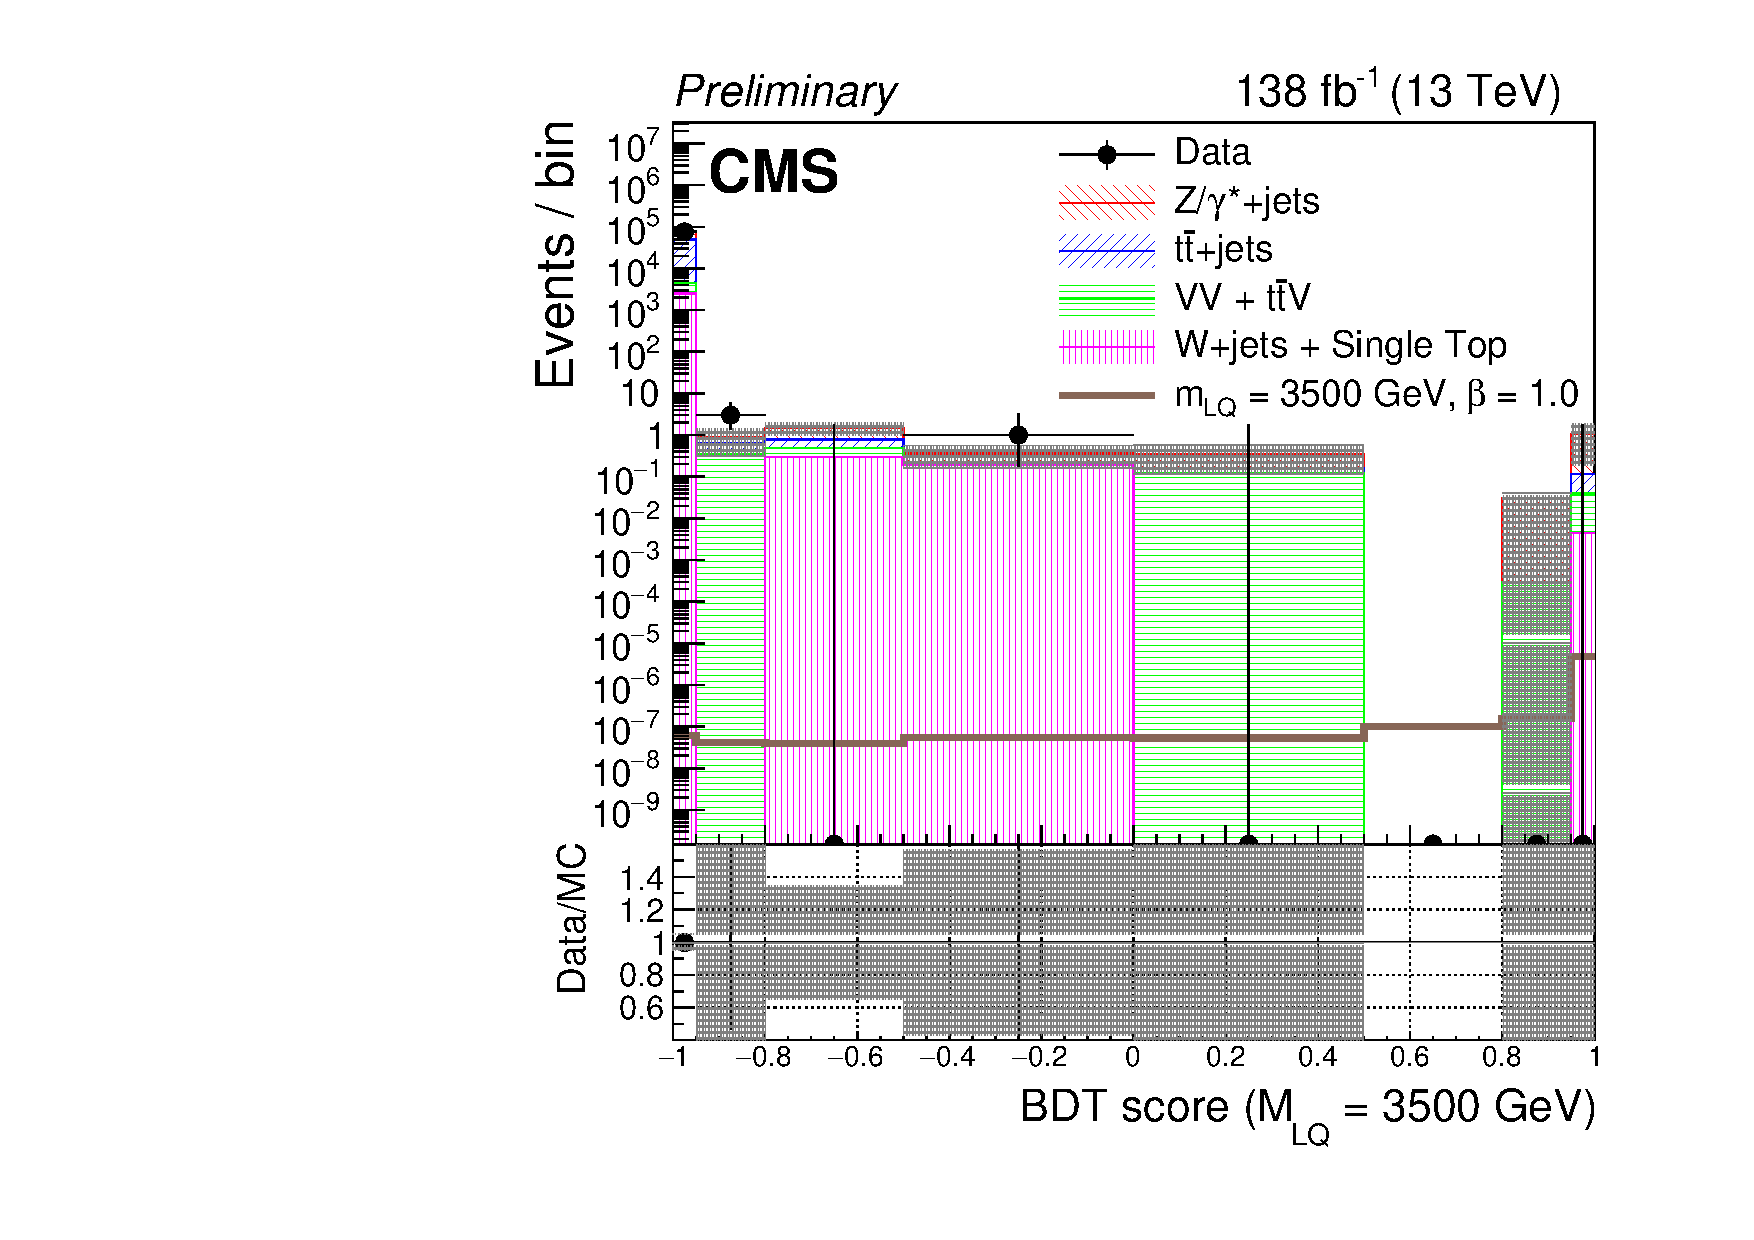
\includegraphics[width=.32\textwidth]{Images/Analysis/Results_combined_Unblinded/Plots/Preselection/BasicLQ_uujj_LQToBMu_pair_uubj_BDT_discrim_M3500_standard.pdf}}
    {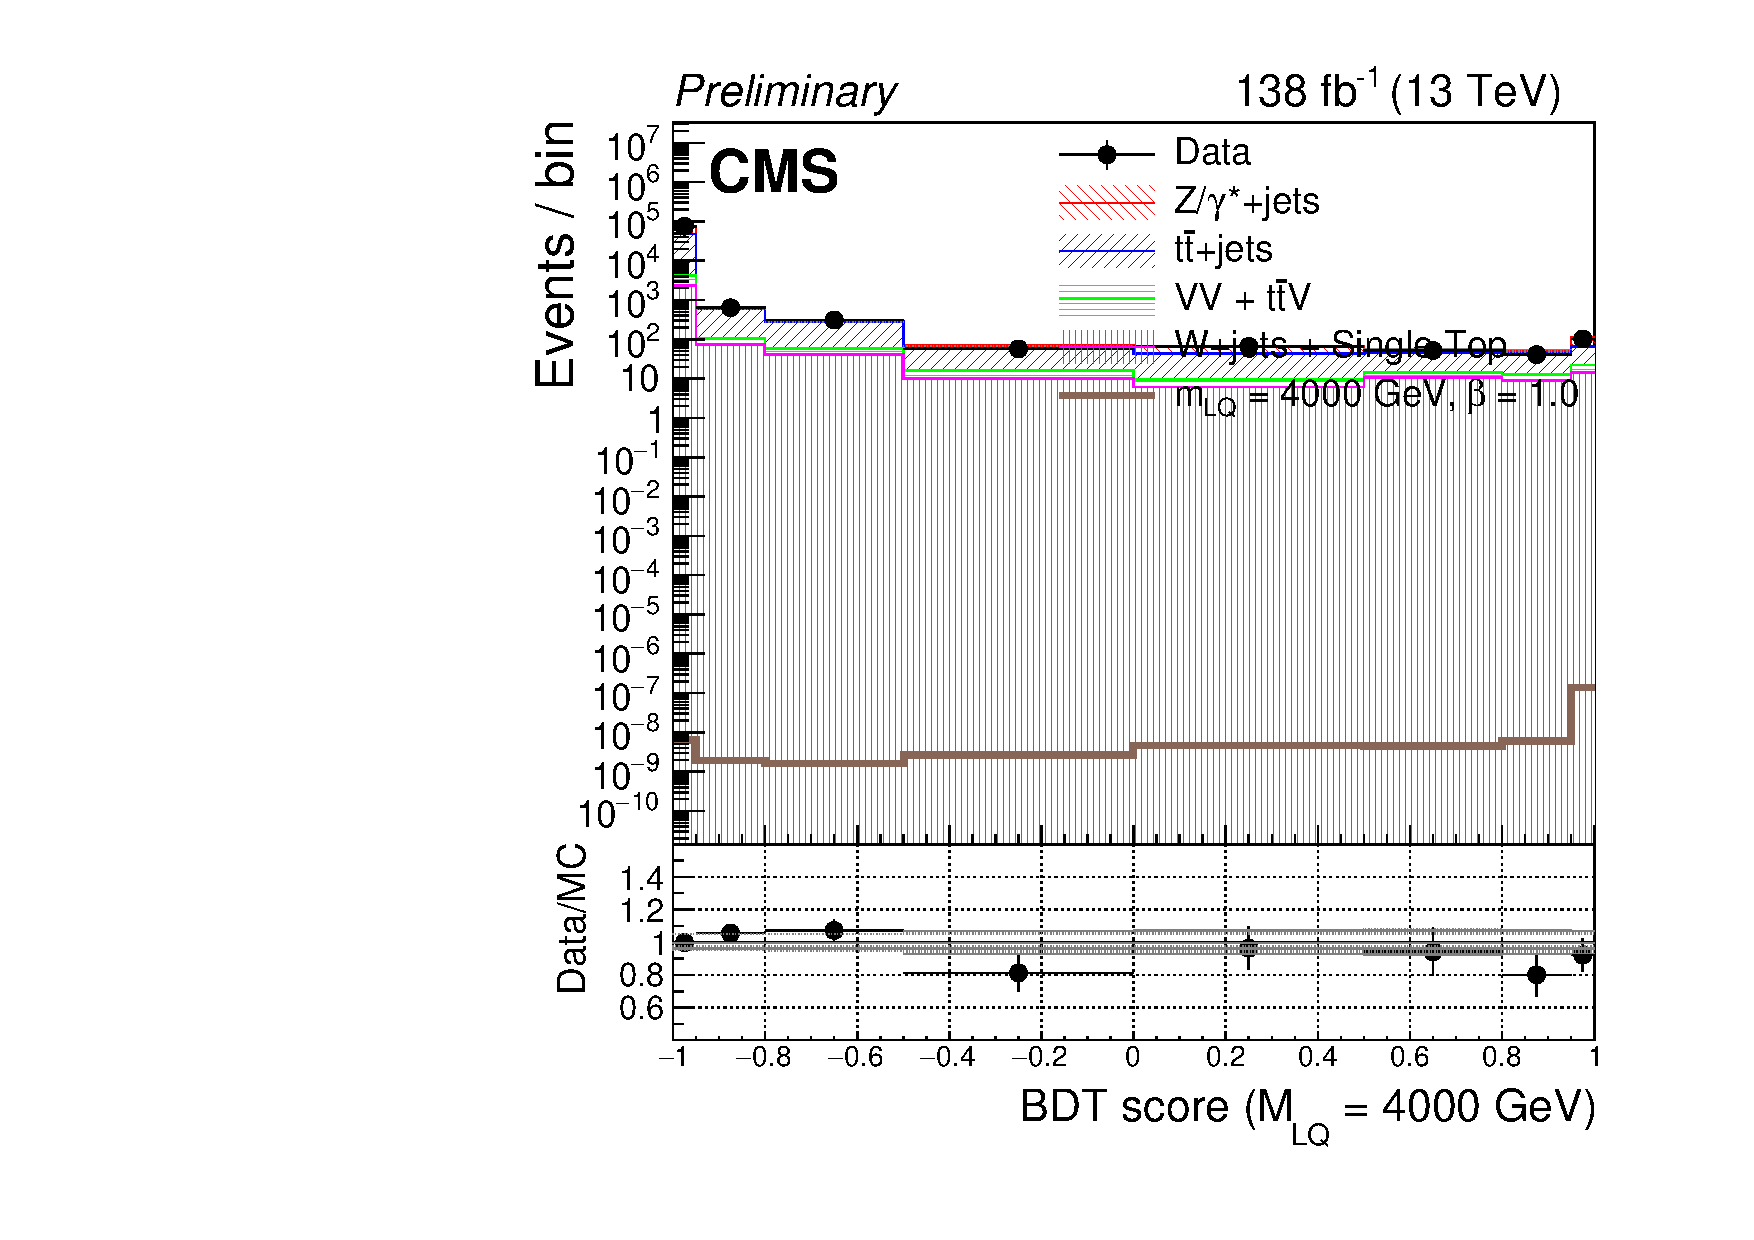
\includegraphics[width=.32\textwidth]{Images/Analysis/Results_combined_Unblinded/Plots/Preselection/BasicLQ_uujj_LQToBMu_pair_uubj_BDT_discrim_M4000_standard.pdf}}

    \caption{A comparison between observed and expected events of BDT responses at preselection level in the combination of 2016, 2017, and 2018 data. The leptoquark mass of the signal in each plot corresponds to the leptoquark mass used in the BDT training. Error bars represent statistical uncertainties, while the shaded area represents systematic uncertainties.
    \label{figapp:BDT2700to4000}}
\end{figure}

\begin{figure}[H]
    \centering
    {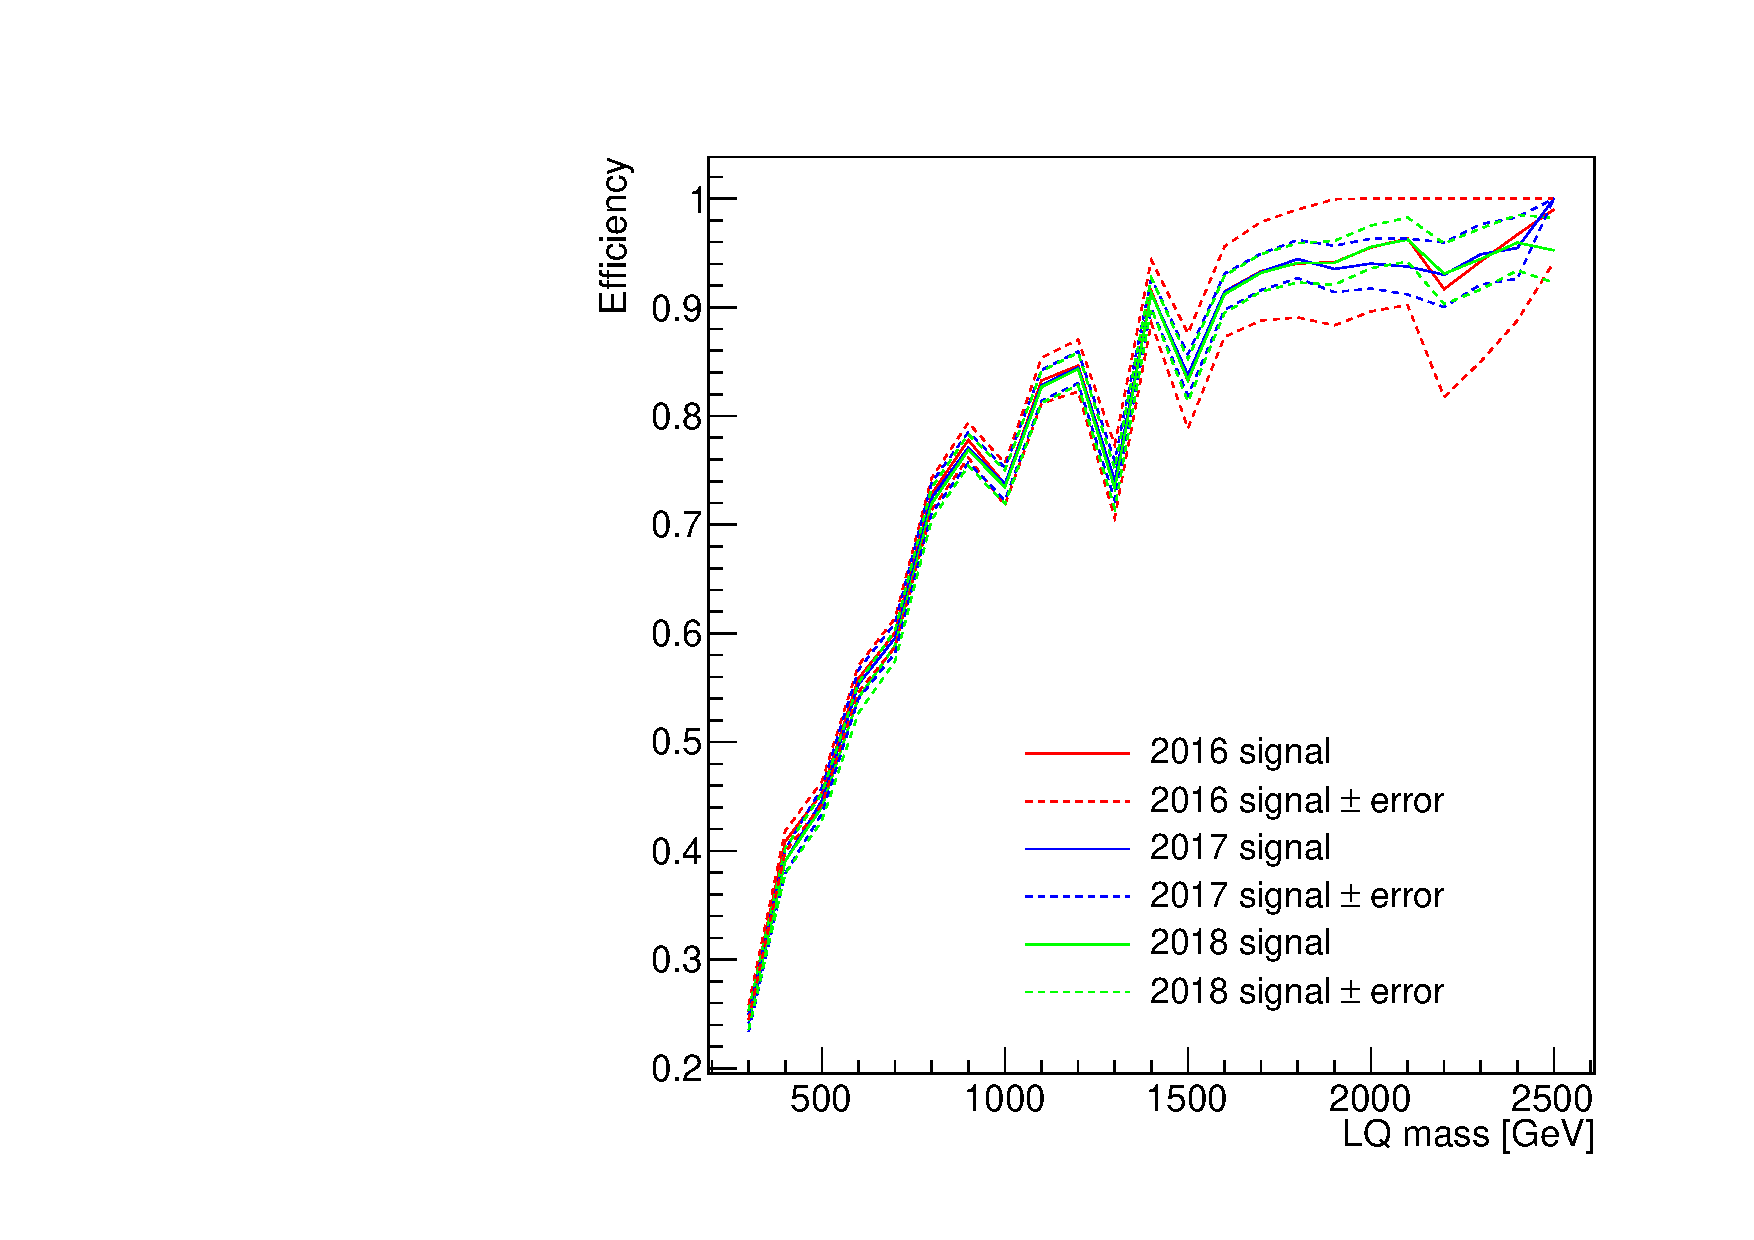
\includegraphics[width=.49\textwidth]{Images/Analysis/finalSelectionEfficiencies_TGraphAsymmErrors_Signal.pdf}}
    {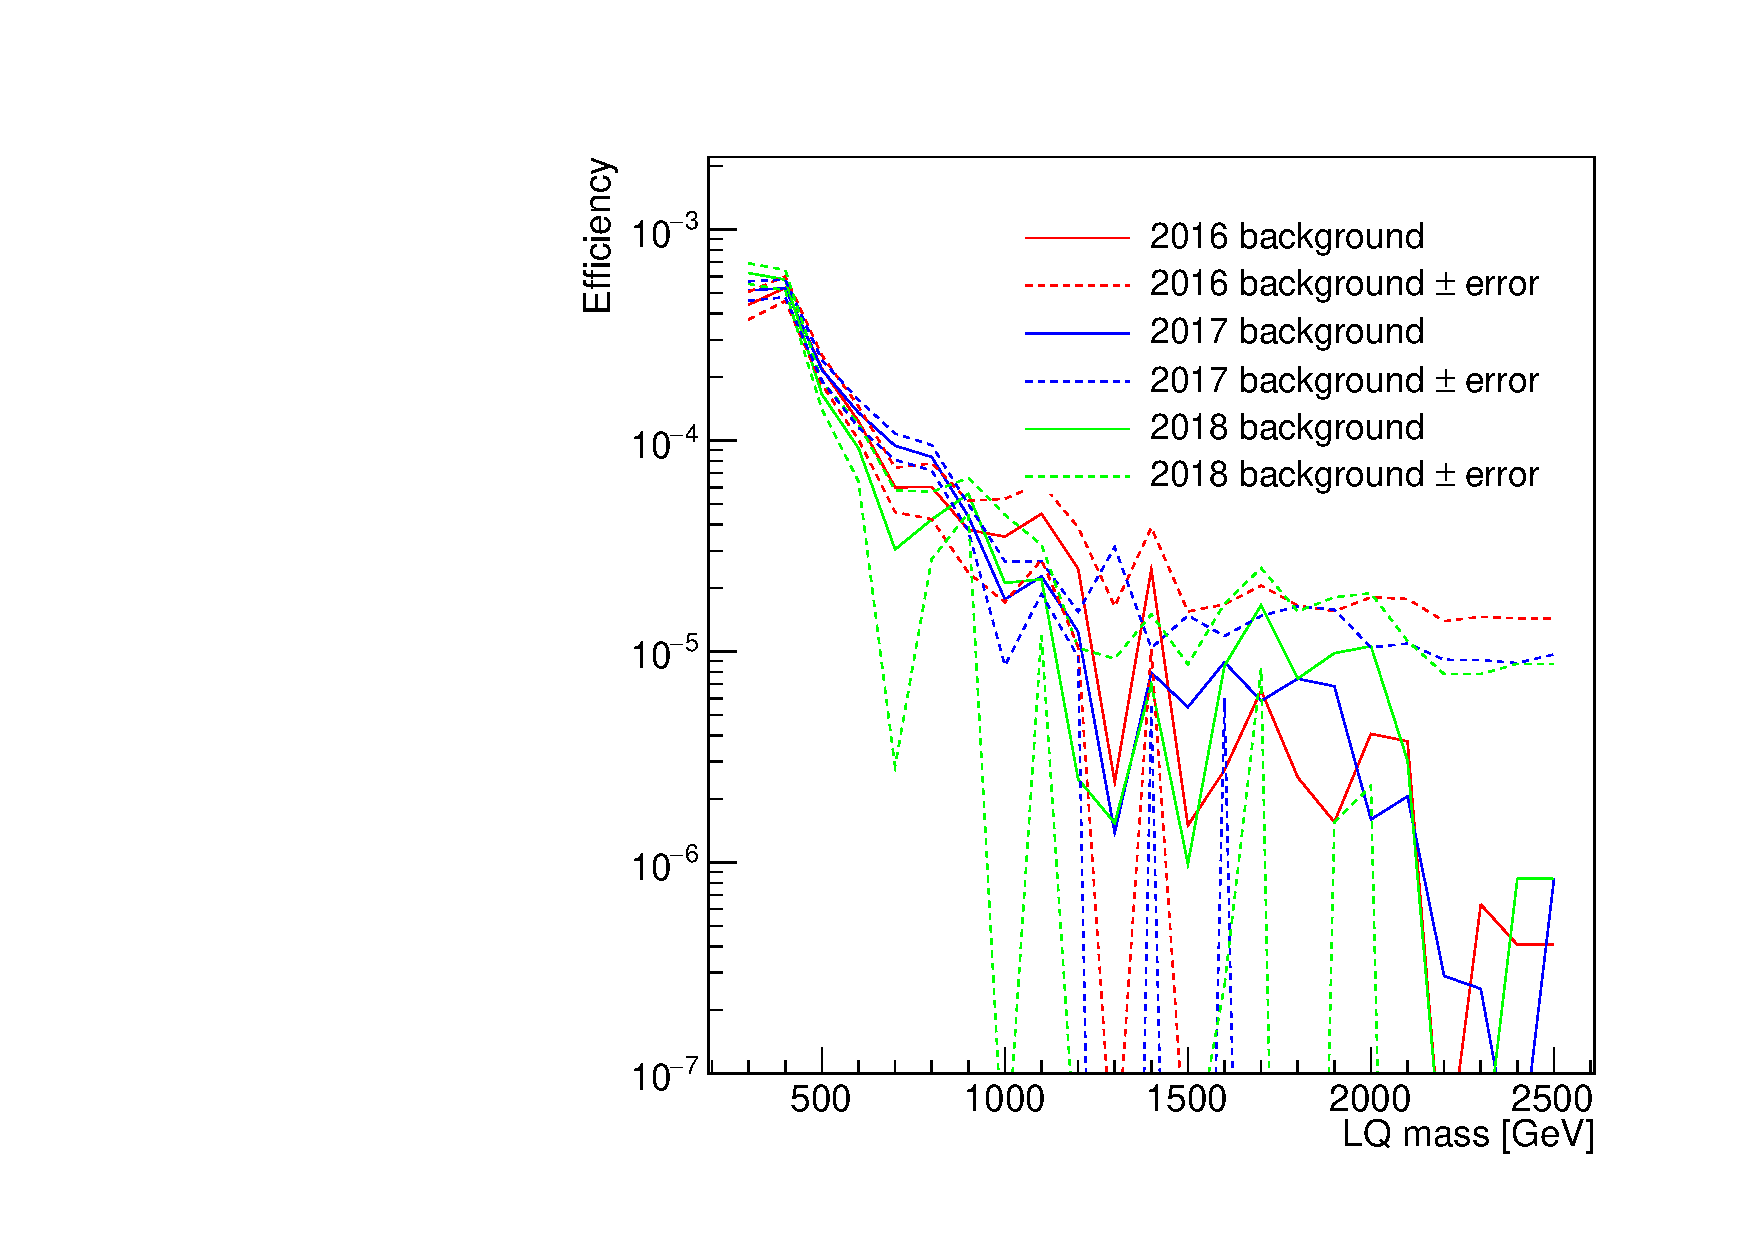
\includegraphics[width=.49\textwidth]{Images/Analysis/finalSelectionEfficiencies_TGraphAsymmErrors_Background.pdf}}
    \caption{The signal (left) and background (right) efficiencies in 2016, 2017, and 2018 MC after applying each final selection cut as a function of leptoquark mass. Dashed lines are error bands that combine systematic and statistical uncertainties.
    \label{figapp:efficiency}}
\end{figure}

\begin{table}[H]
    \caption{Final selection cuts are defined for each leptoquark mass point consisting of the optimized cut on the BDT discriminant, a flat cut on \Muu, and a LQ-mass-dependent cut \Muujj.}
    \begin{center}
        \begin{scriptsize}
            \begin{tabular}{lccc} \hline\hline
                Leptoquark mass [\GeV]  & \multicolumn{3}{c}{Final selection cuts} \\
                                & BDT score & \Muujj [\GeV]  & \Muu [\GeV] \\ \hline
                300             & 0.978     & 300           & 250 \\
                400             & 0.99      & 400           & 250 \\
                500             & 0.99      & 500           & 250 \\
                600             & 0.994     & 600           & 250 \\
                700             & 0.994     & 700           & 250 \\
                800             & 0.994     & 800           & 250 \\
                900             & 0.993     & 900           & 250 \\
                1000            & 0.993     & 1000          & 250 \\
                1100            & 0.989     & 1100          & 250 \\
                1200            & 0.996     & 1200          & 250 \\
                1300            & 0.996     & 1300          & 250 \\
                1400            & 0.978     & 1400          & 250 \\
                1500            & 0.993     & 1500          & 250 \\
                1600            & 0.987     & 1600          & 250 \\
                1700            & 0.991     & 1700          & 250 \\
                1800            & 0.995     & 1800          & 250 \\
                1900            & 0.964     & 1900          & 250 \\
                2000            & 0.987     & 2000          & 250 \\
                2100            & 0.992     & 2100          & 250 \\
                2200            & 0.998     & 2200          & 250 \\
                2300            & 0.998     & 2300          & 250 \\
                2400            & 0.998     & 2400          & 250 \\
                2500            & 0.969     & 2500          & 250 \\
                2600            & 0.949     & 2600          & 250 \\
                2700            & 0.977     & 2700          & 250 \\
                2800            & 0.982     & 2800          & 250 \\
                2900            & 0.996     & 2900          & 250 \\
                3000            & 0.998     & 3000          & 250 \\
                3500            & 0.989     & 3500          & 250 \\
                4000            & 0.999     & 4000          & 250 \\ \hline\hline
            \end{tabular}
            \label{tab:cutlog}
        \end{scriptsize}
    \end{center}
\end{table}

\begin{figure}[H]
    \centering
    {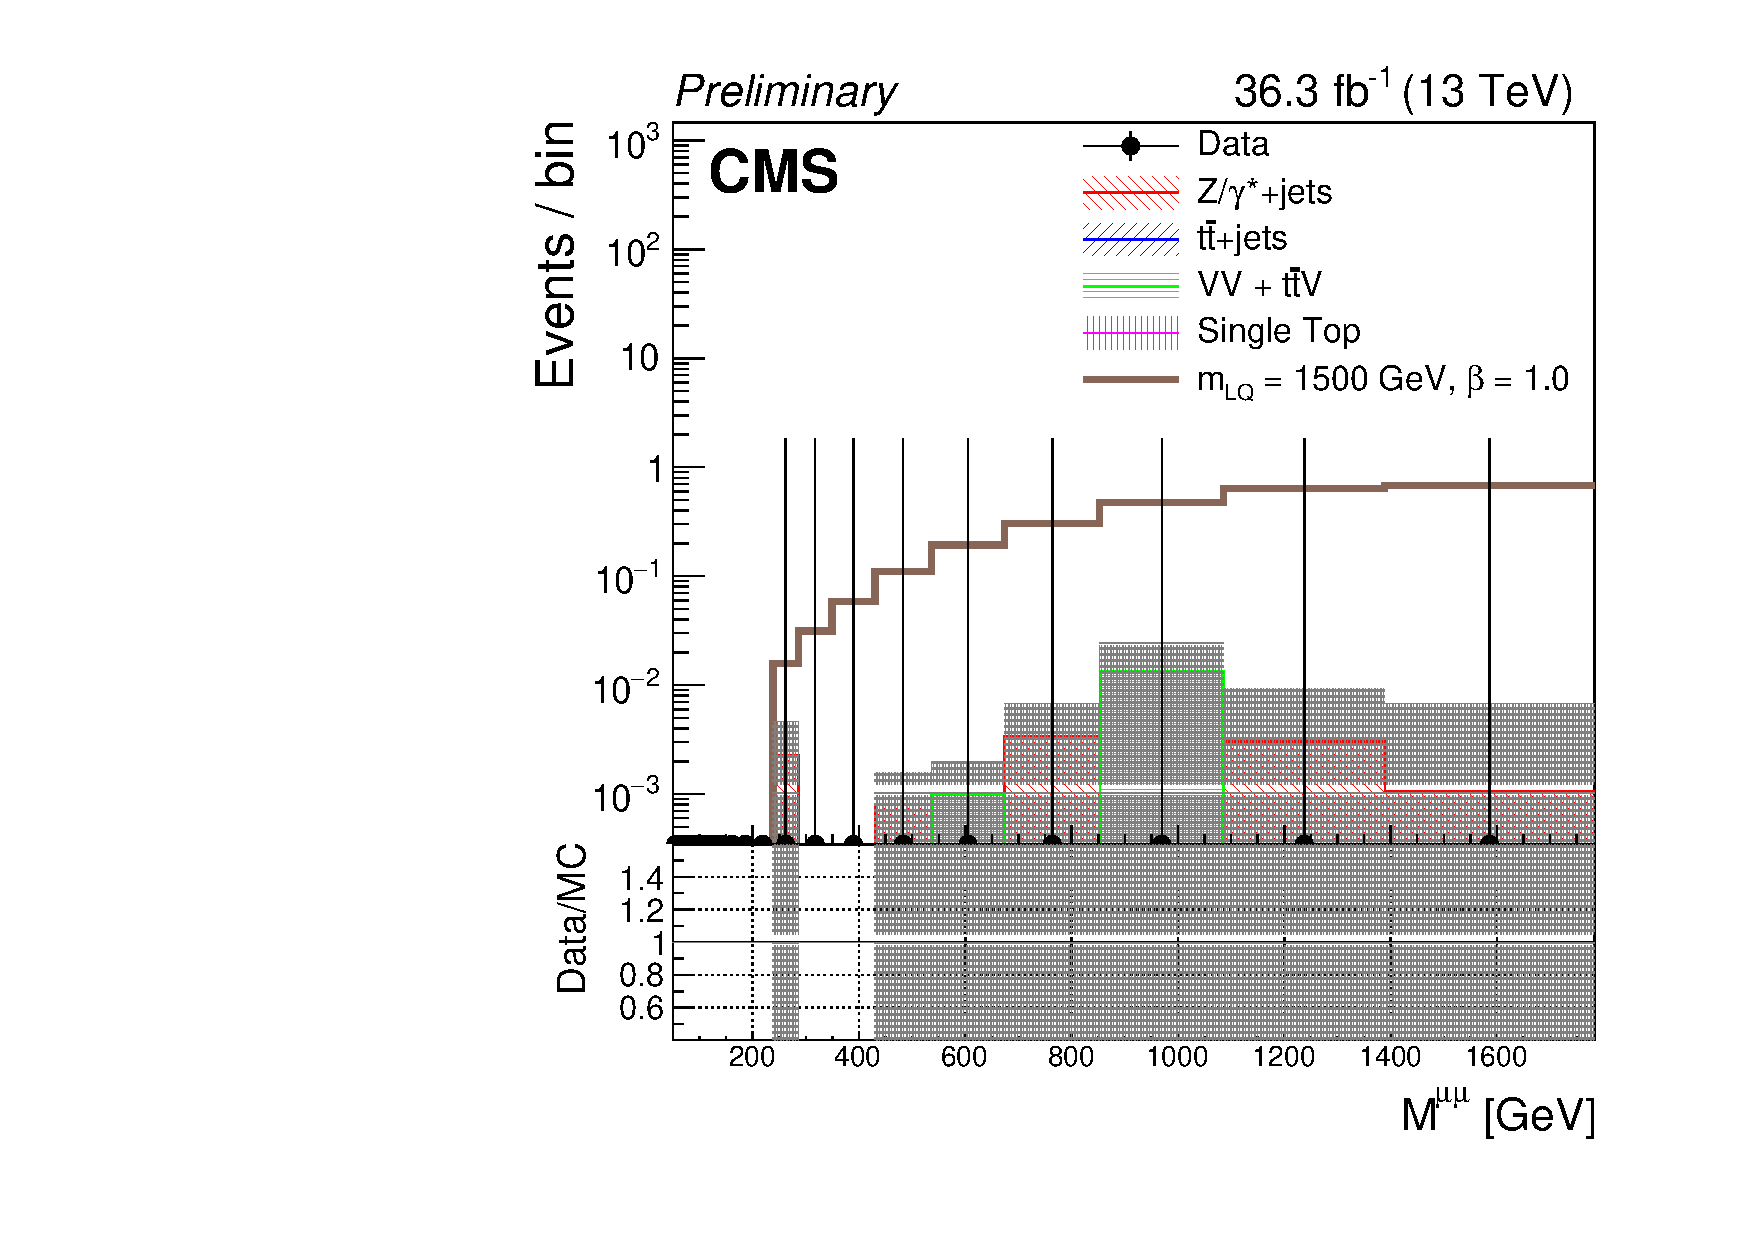
\includegraphics[width=.32\textwidth]{Images/Analysis/Results_2016_Unblinded/Plots/Final_selection/BasicLQ_uujj_M_uu_final1500.pdf}}
    {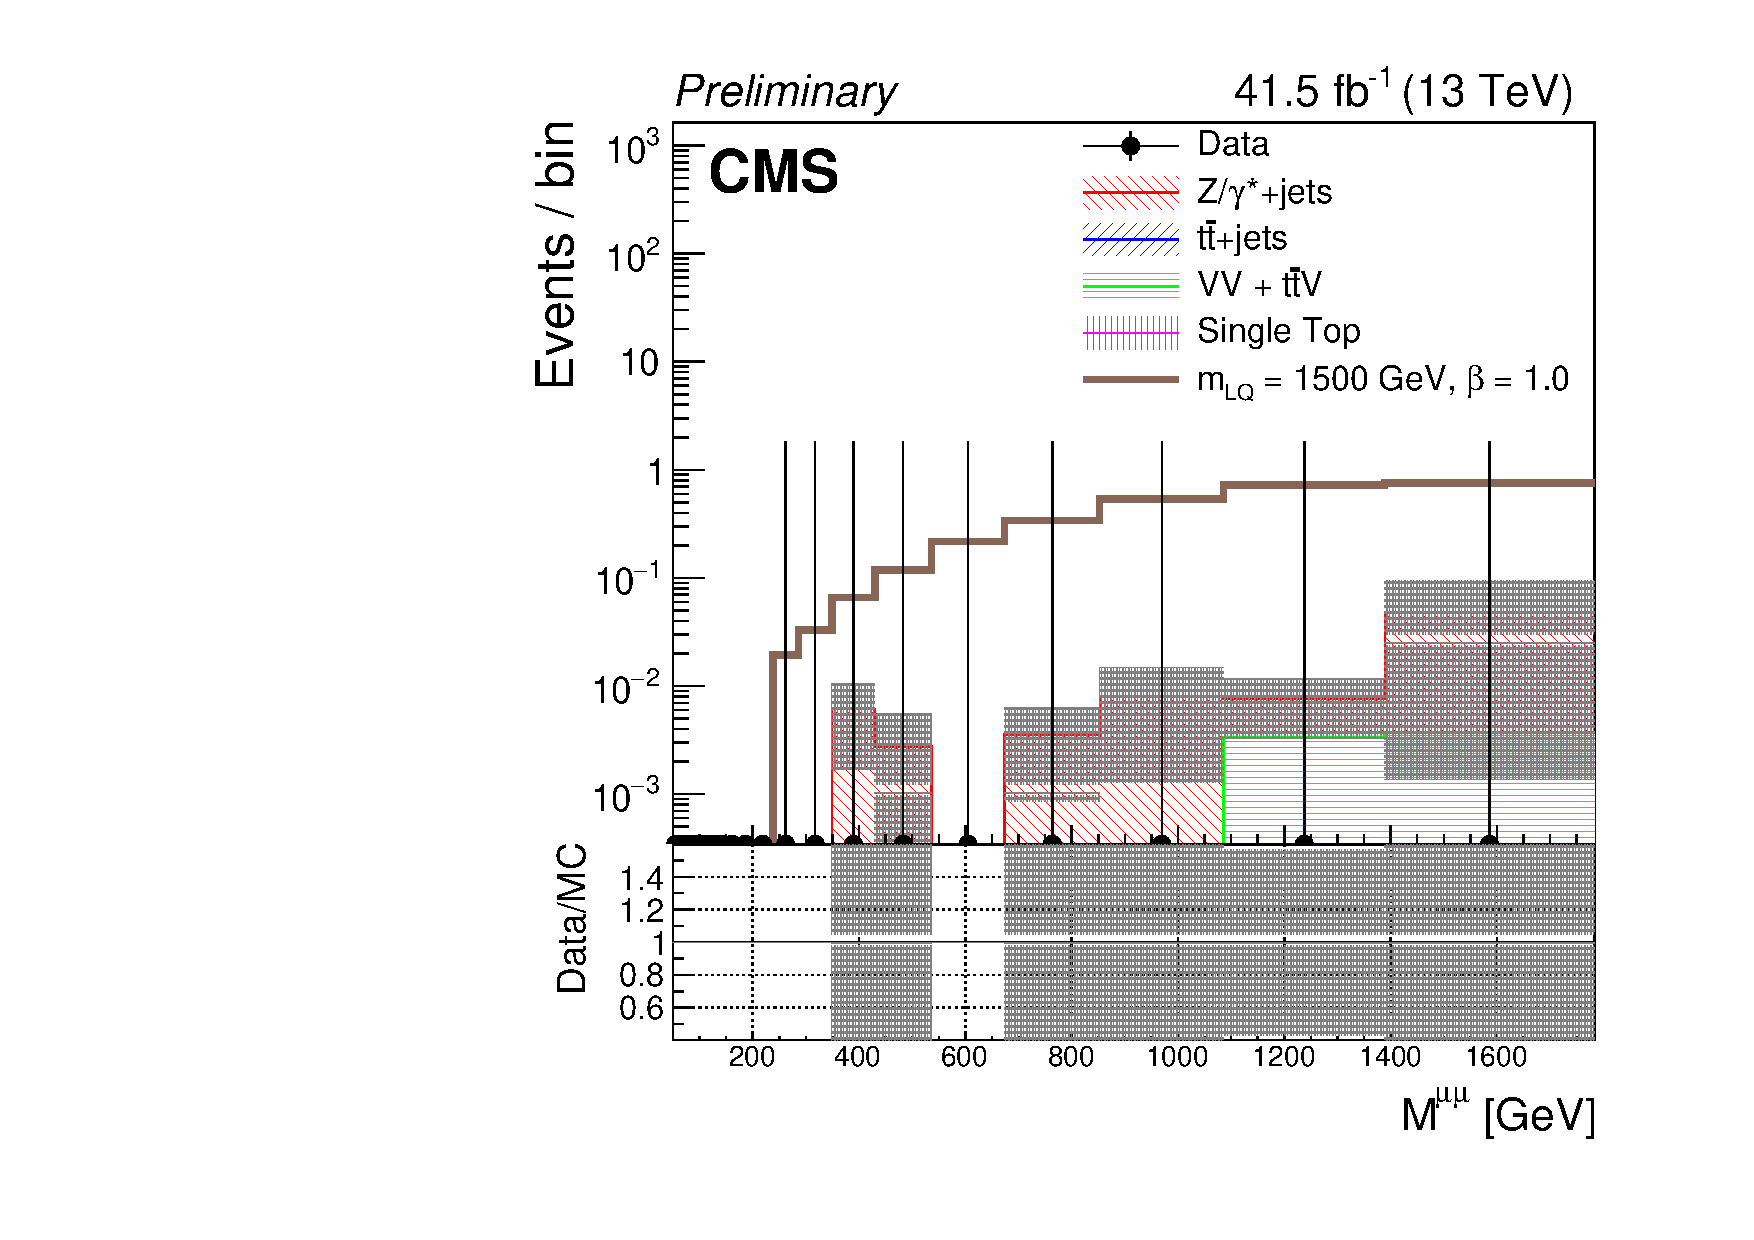
\includegraphics[width=.32\textwidth]{Images/Analysis/Results_2017_Unblinded/Plots/Final_selection/BasicLQ_uujj_M_uu_final1500.pdf}}
    {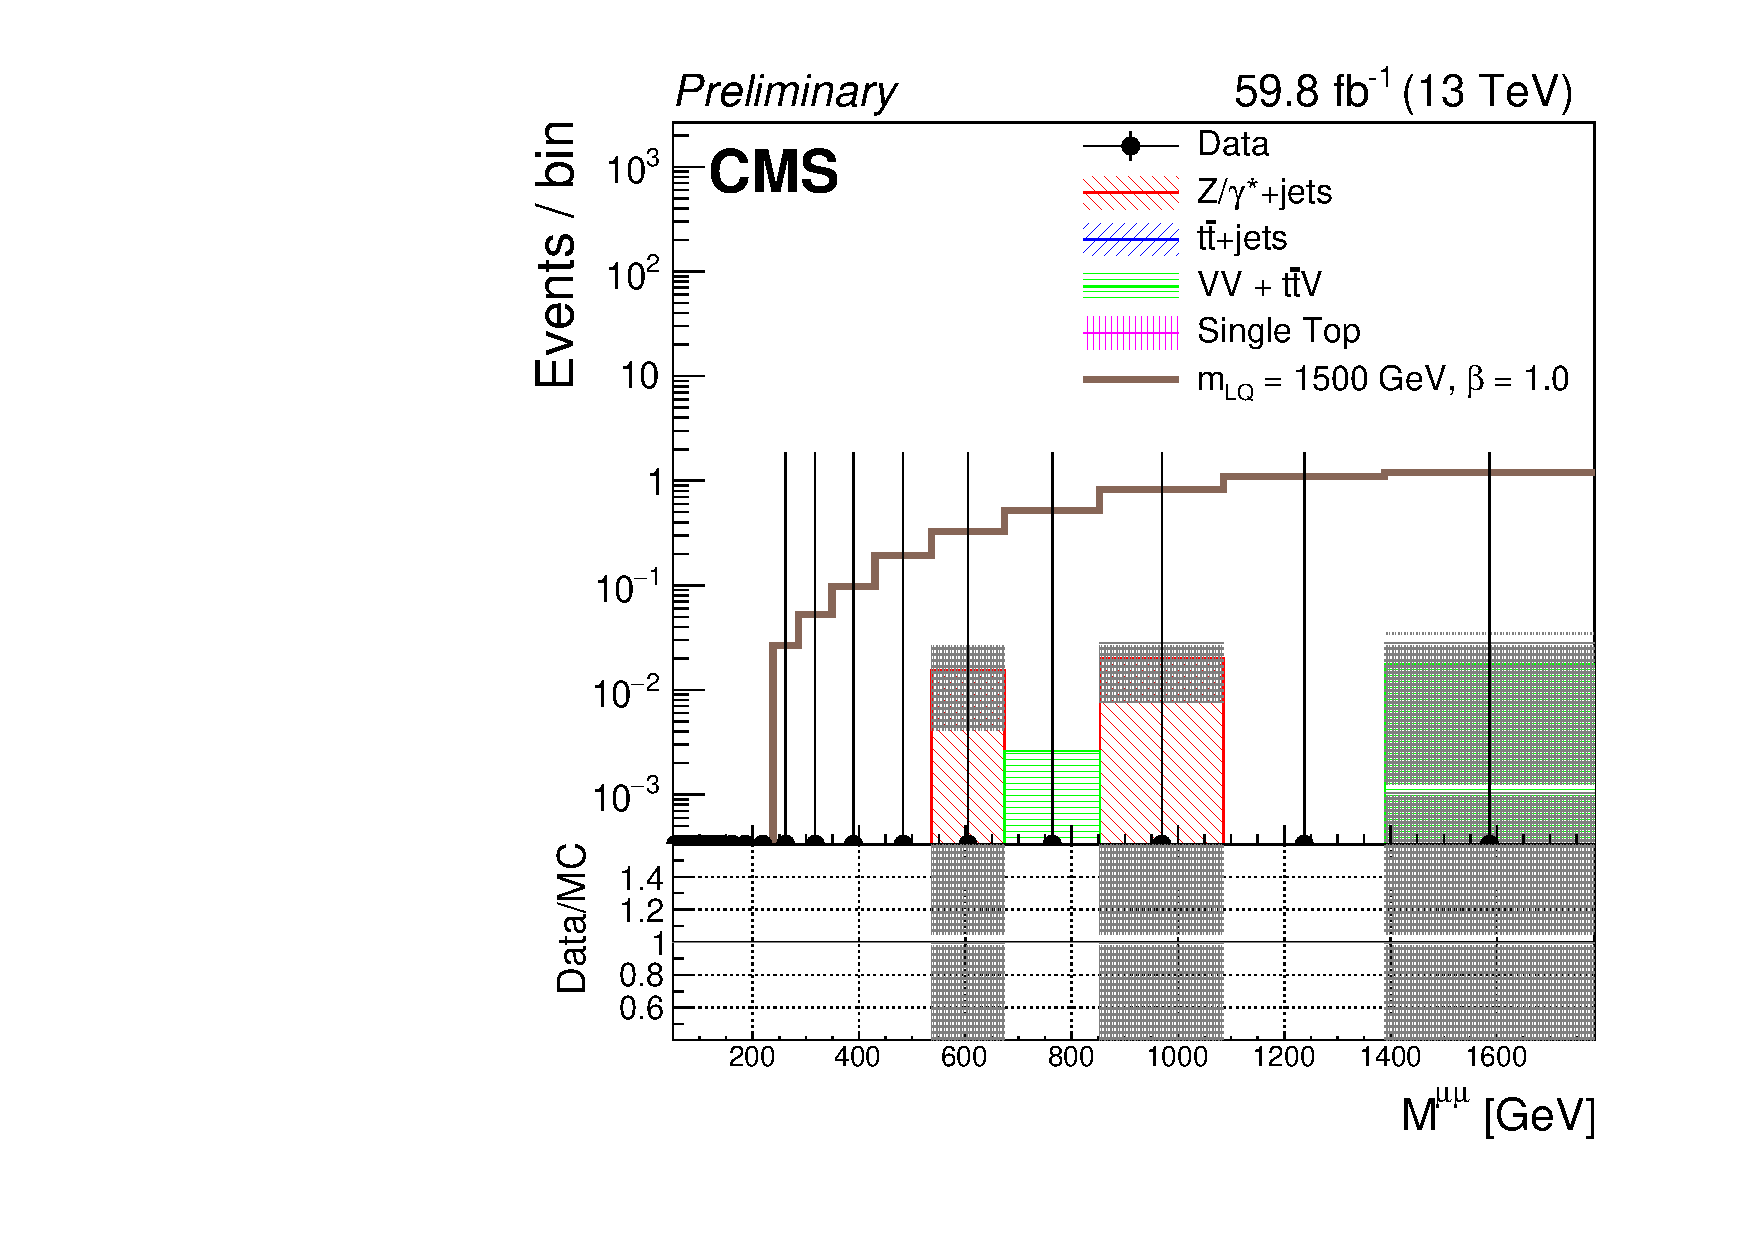
\includegraphics[width=.32\textwidth]{Images/Analysis/Results_2018_Unblinded/Plots/Final_selection/BasicLQ_uujj_M_uu_final1500.pdf}}
    {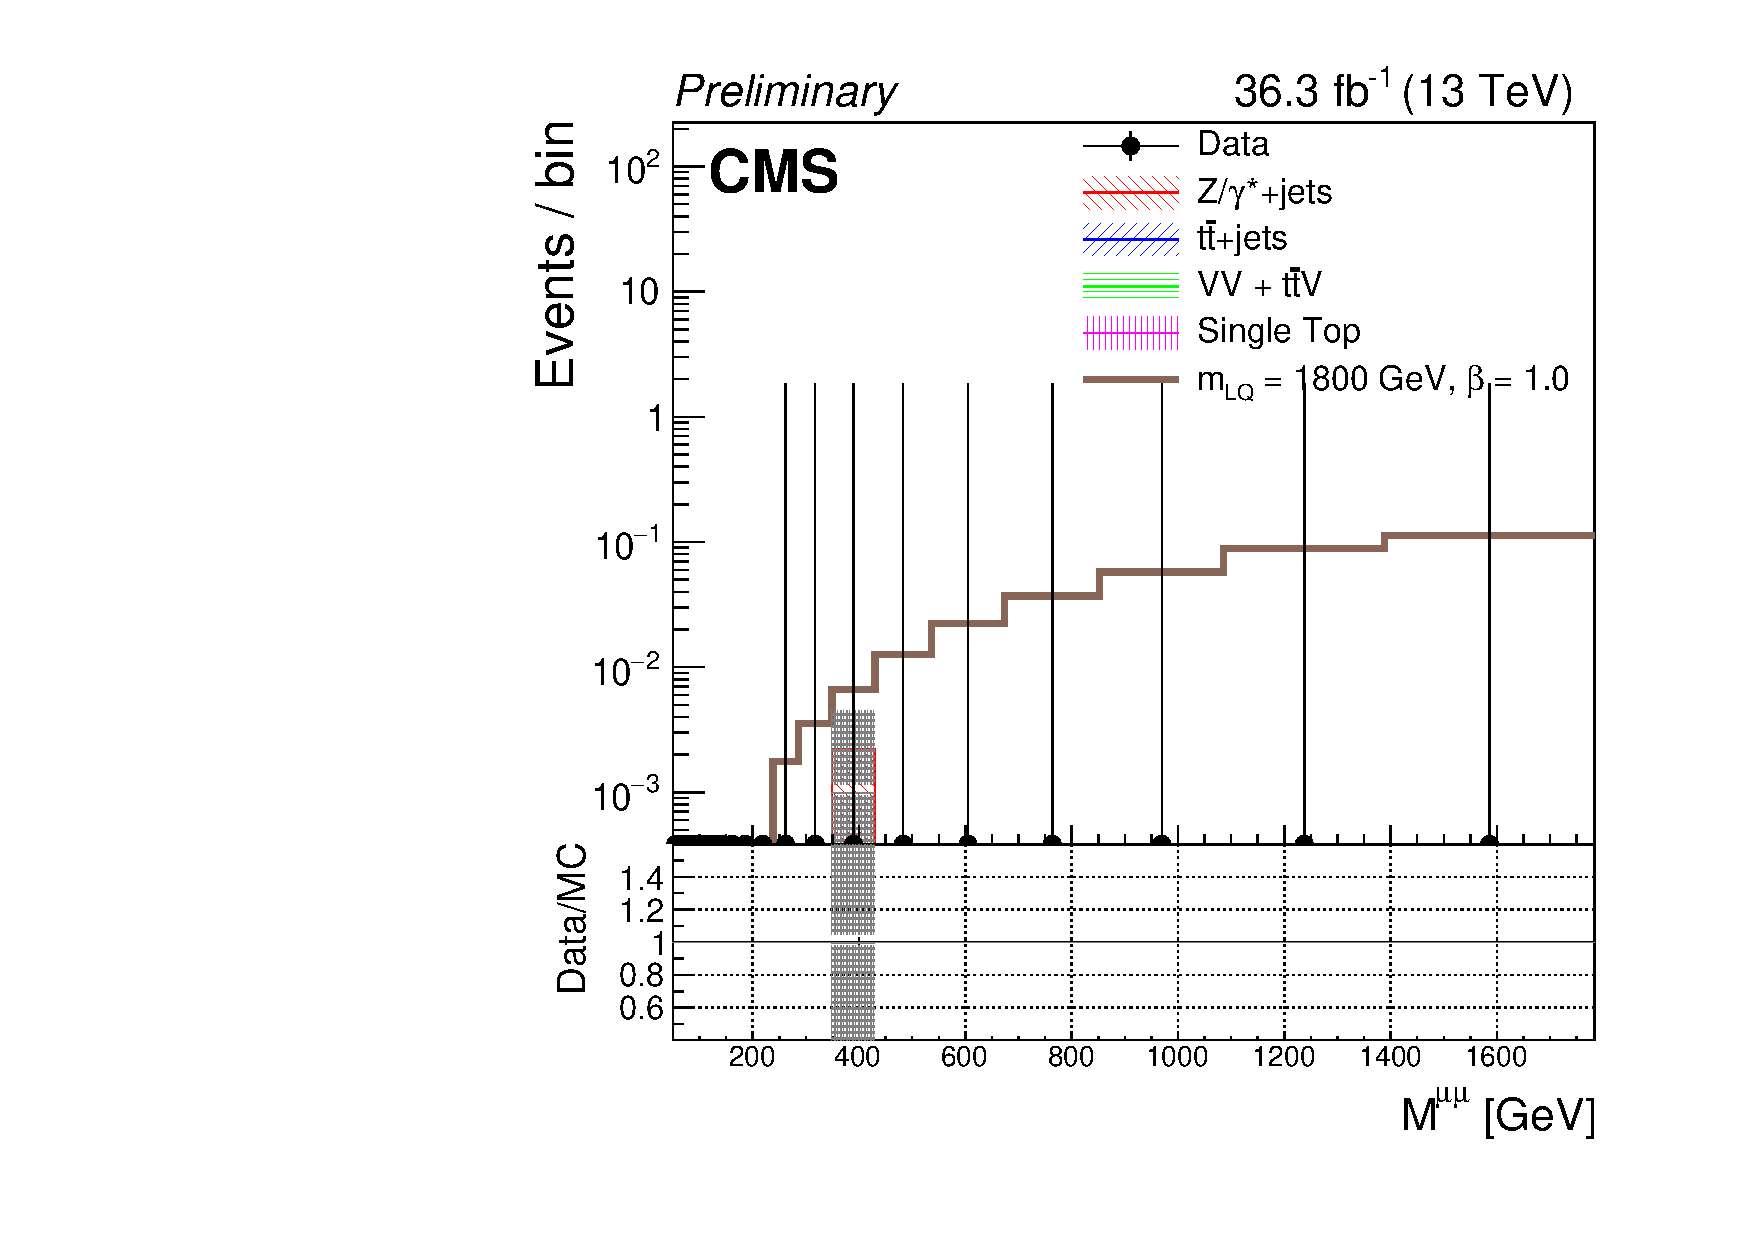
\includegraphics[width=.32\textwidth]{Images/Analysis/Results_2016_Unblinded/Plots/Final_selection/BasicLQ_uujj_M_uu_final1800.pdf}}
    {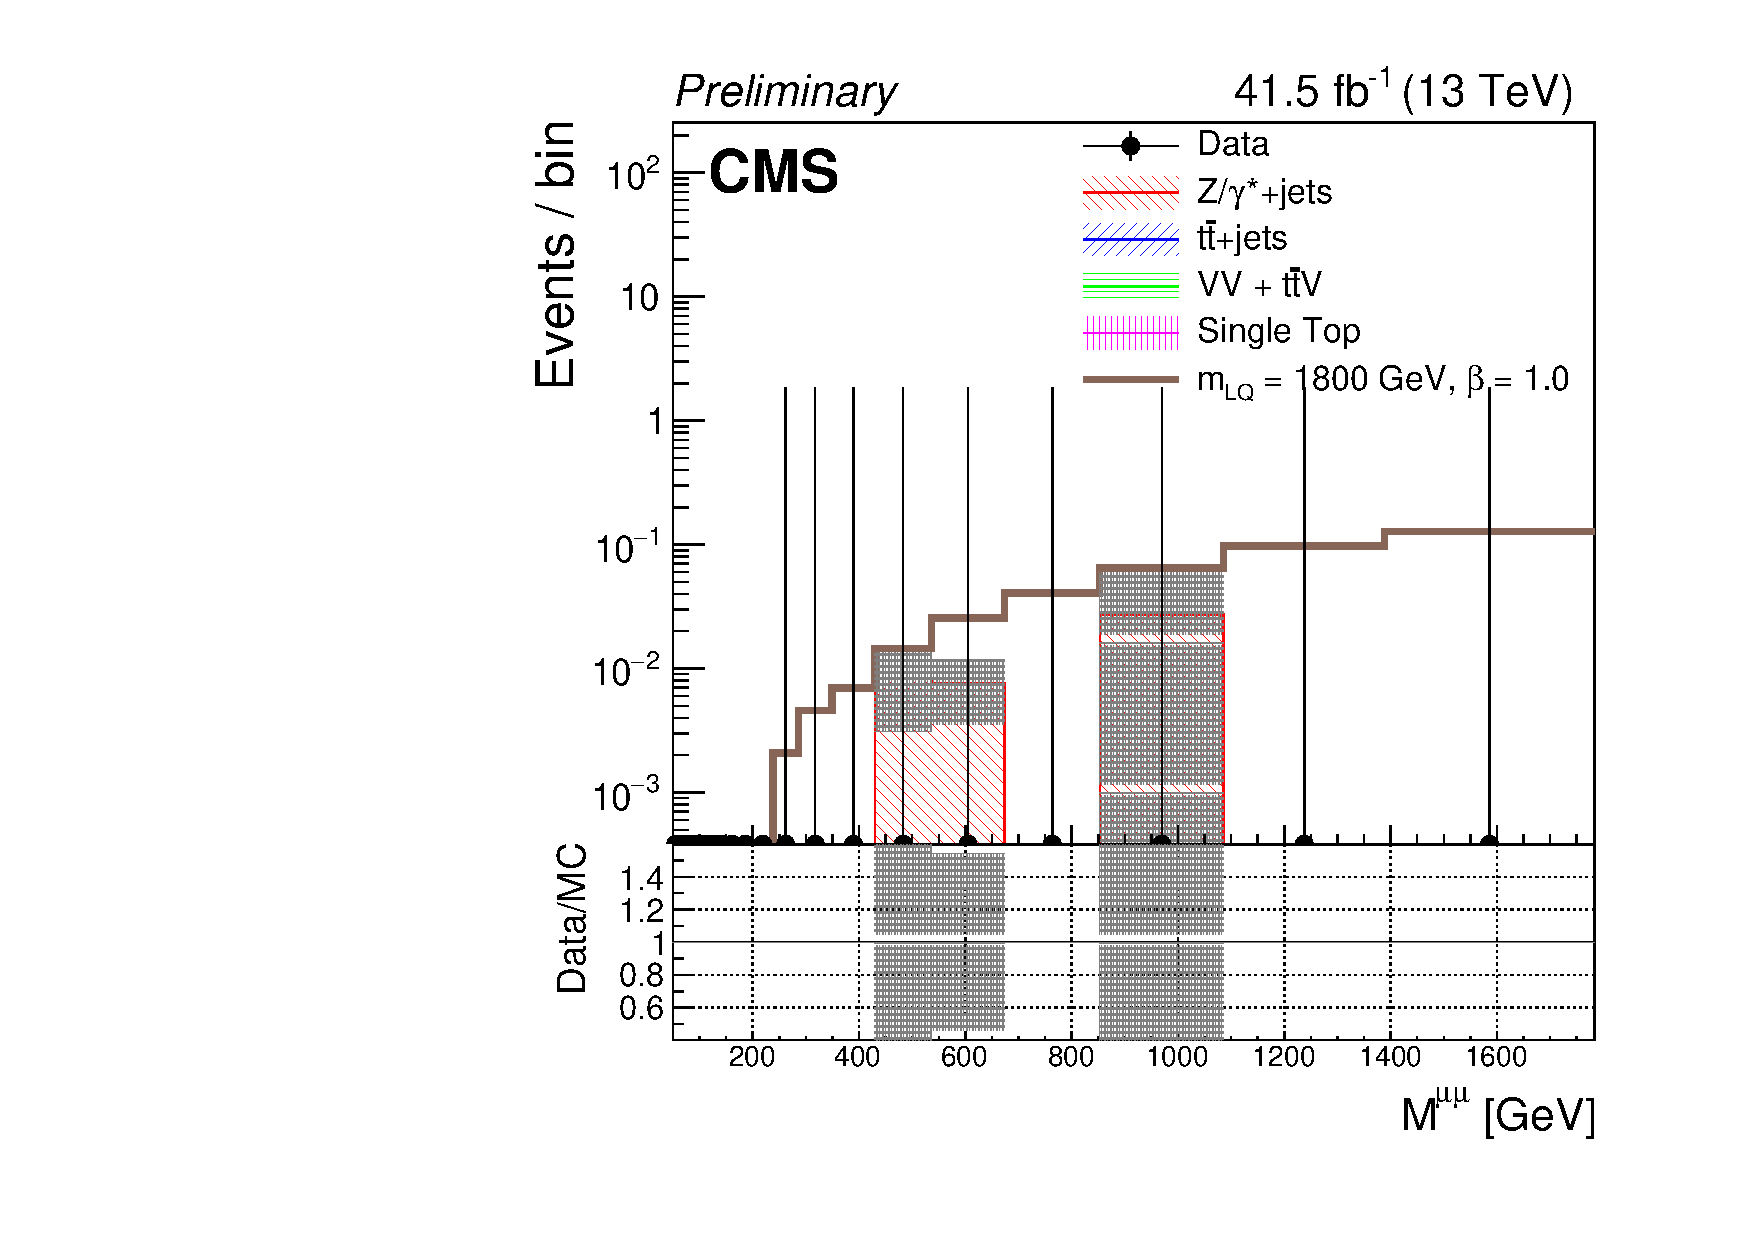
\includegraphics[width=.32\textwidth]{Images/Analysis/Results_2017_Unblinded/Plots/Final_selection/BasicLQ_uujj_M_uu_final1800.pdf}}
    {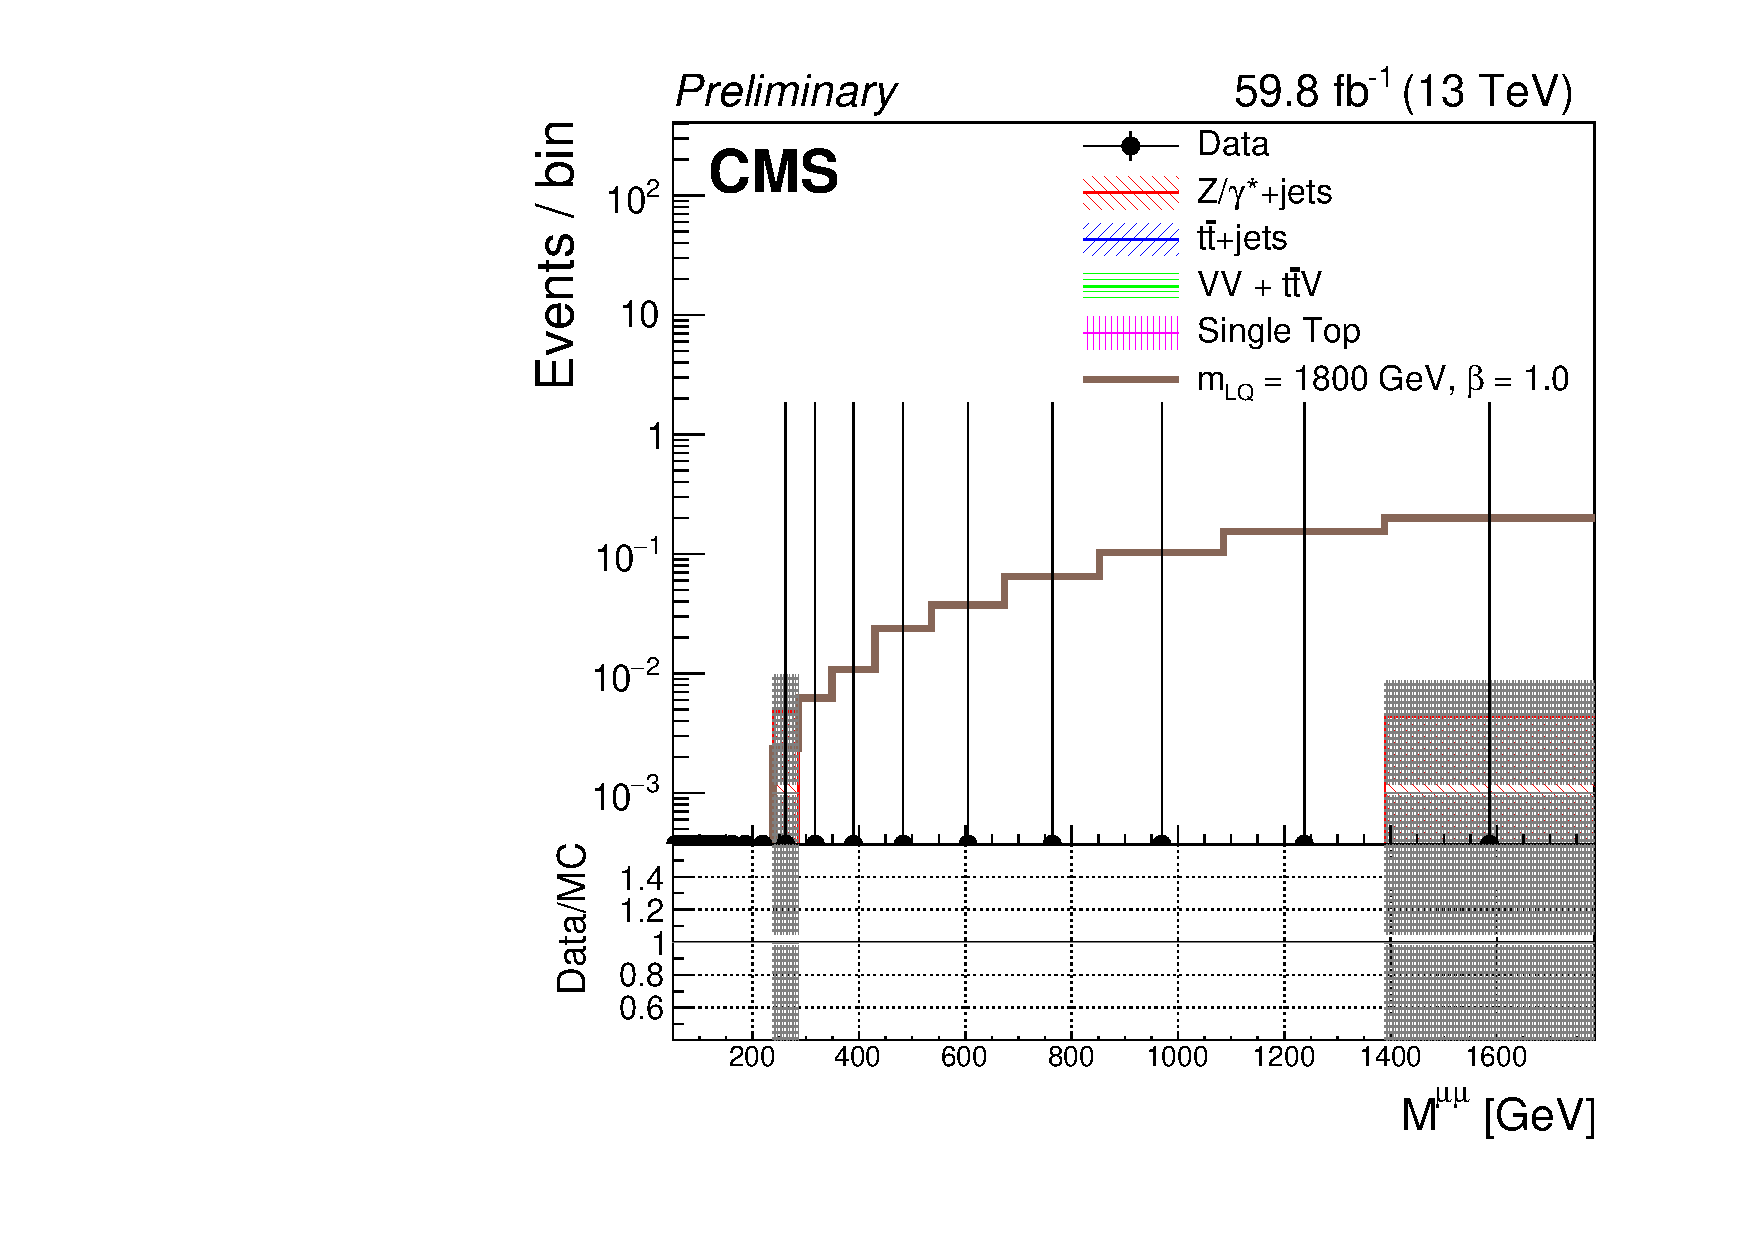
\includegraphics[width=.32\textwidth]{Images/Analysis/Results_2018_Unblinded/Plots/Final_selection/BasicLQ_uujj_M_uu_final1800.pdf}}
    {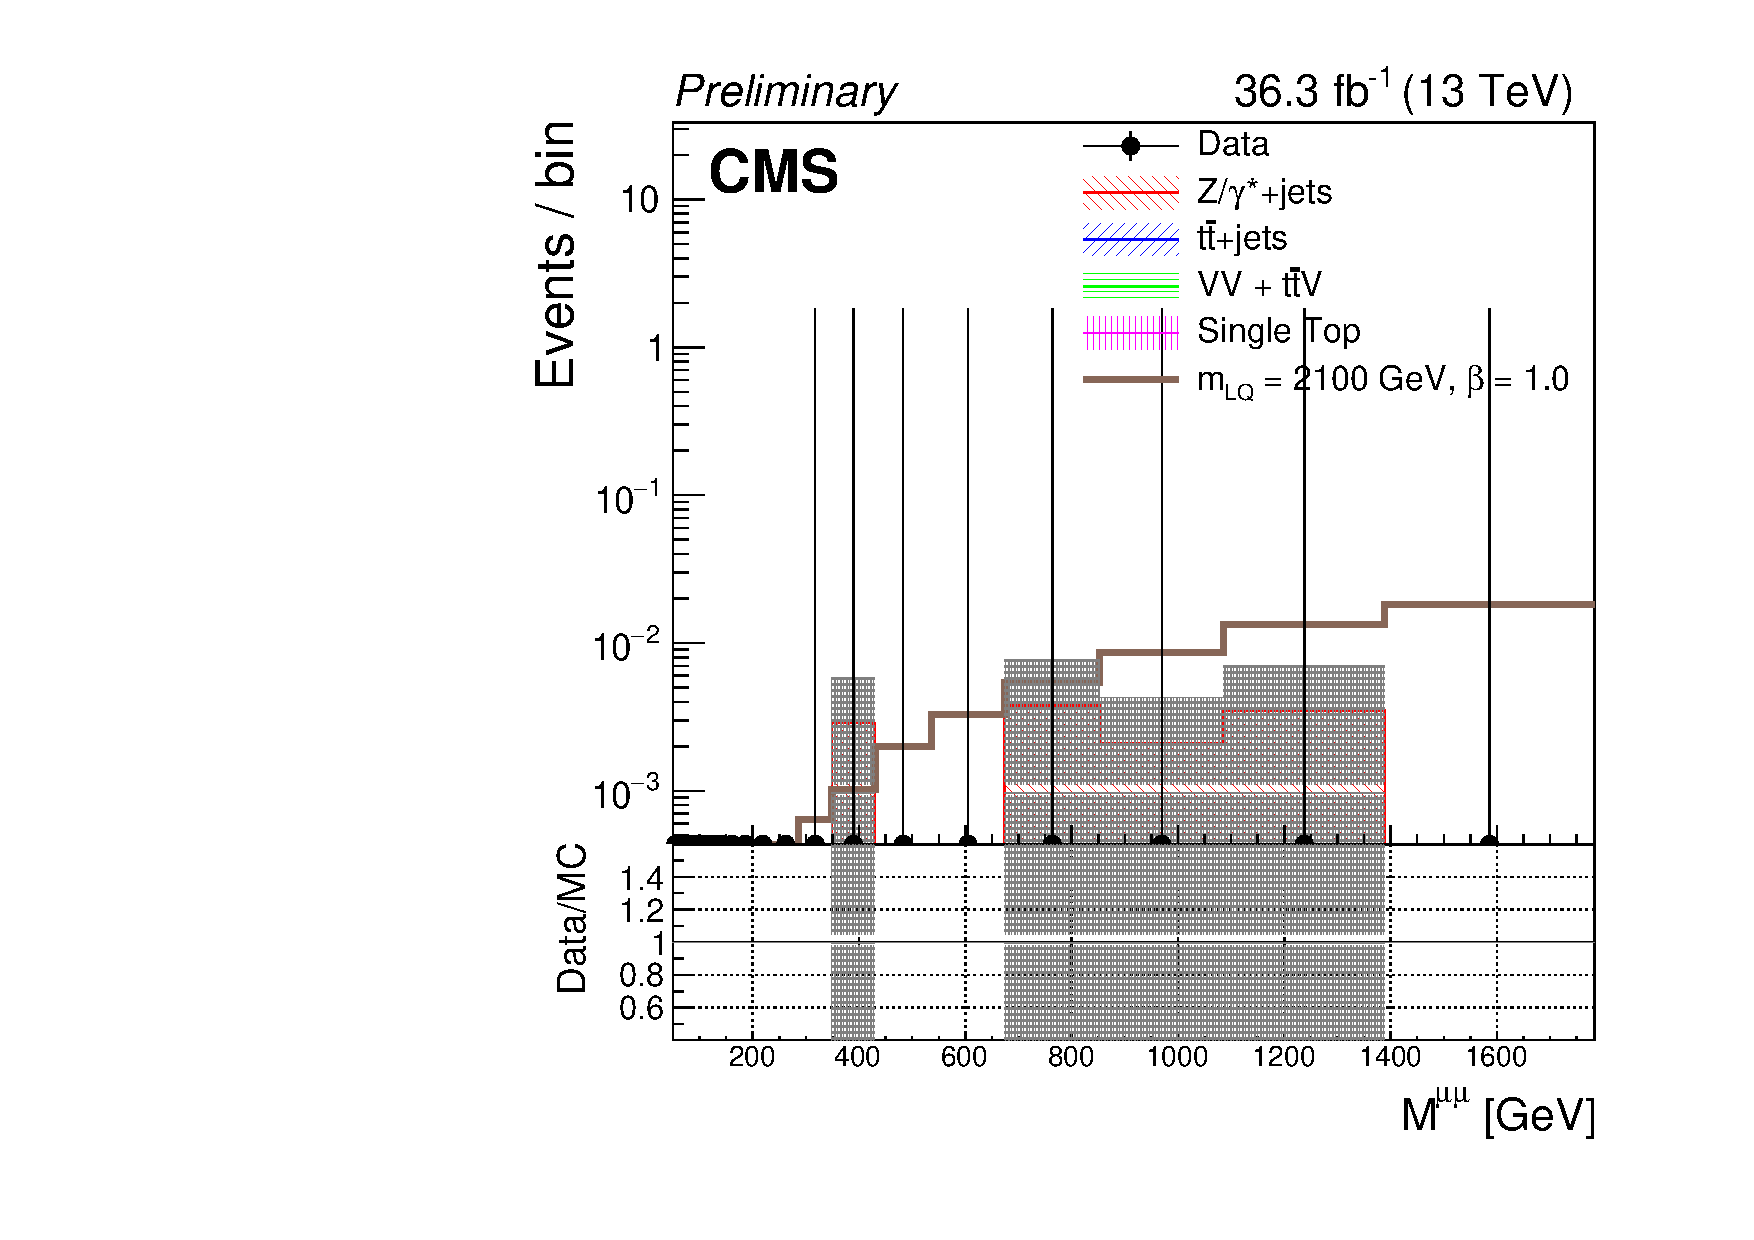
\includegraphics[width=.32\textwidth]{Images/Analysis/Results_2016_Unblinded/Plots/Final_selection/BasicLQ_uujj_M_uu_final2100.pdf}}
    {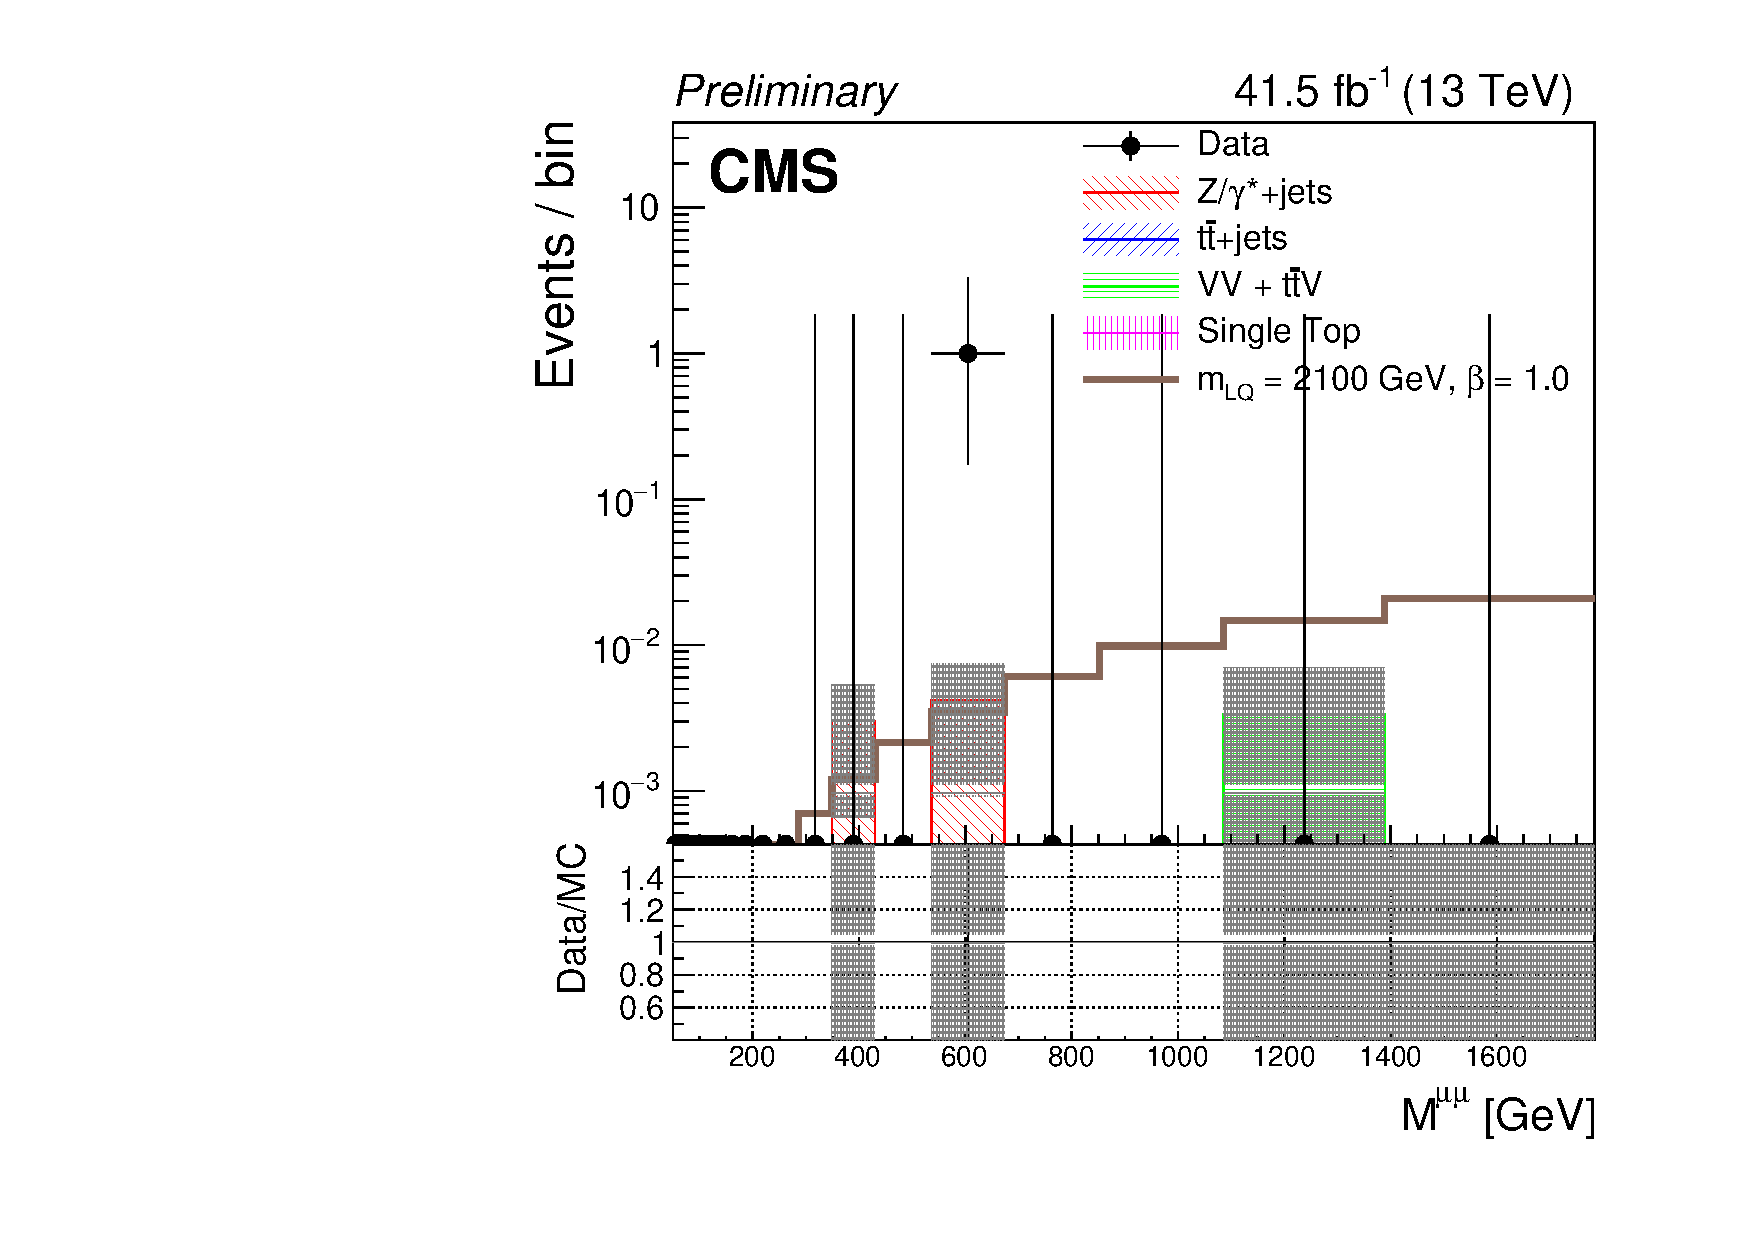
\includegraphics[width=.32\textwidth]{Images/Analysis/Results_2017_Unblinded/Plots/Final_selection/BasicLQ_uujj_M_uu_final2100.pdf}}
    {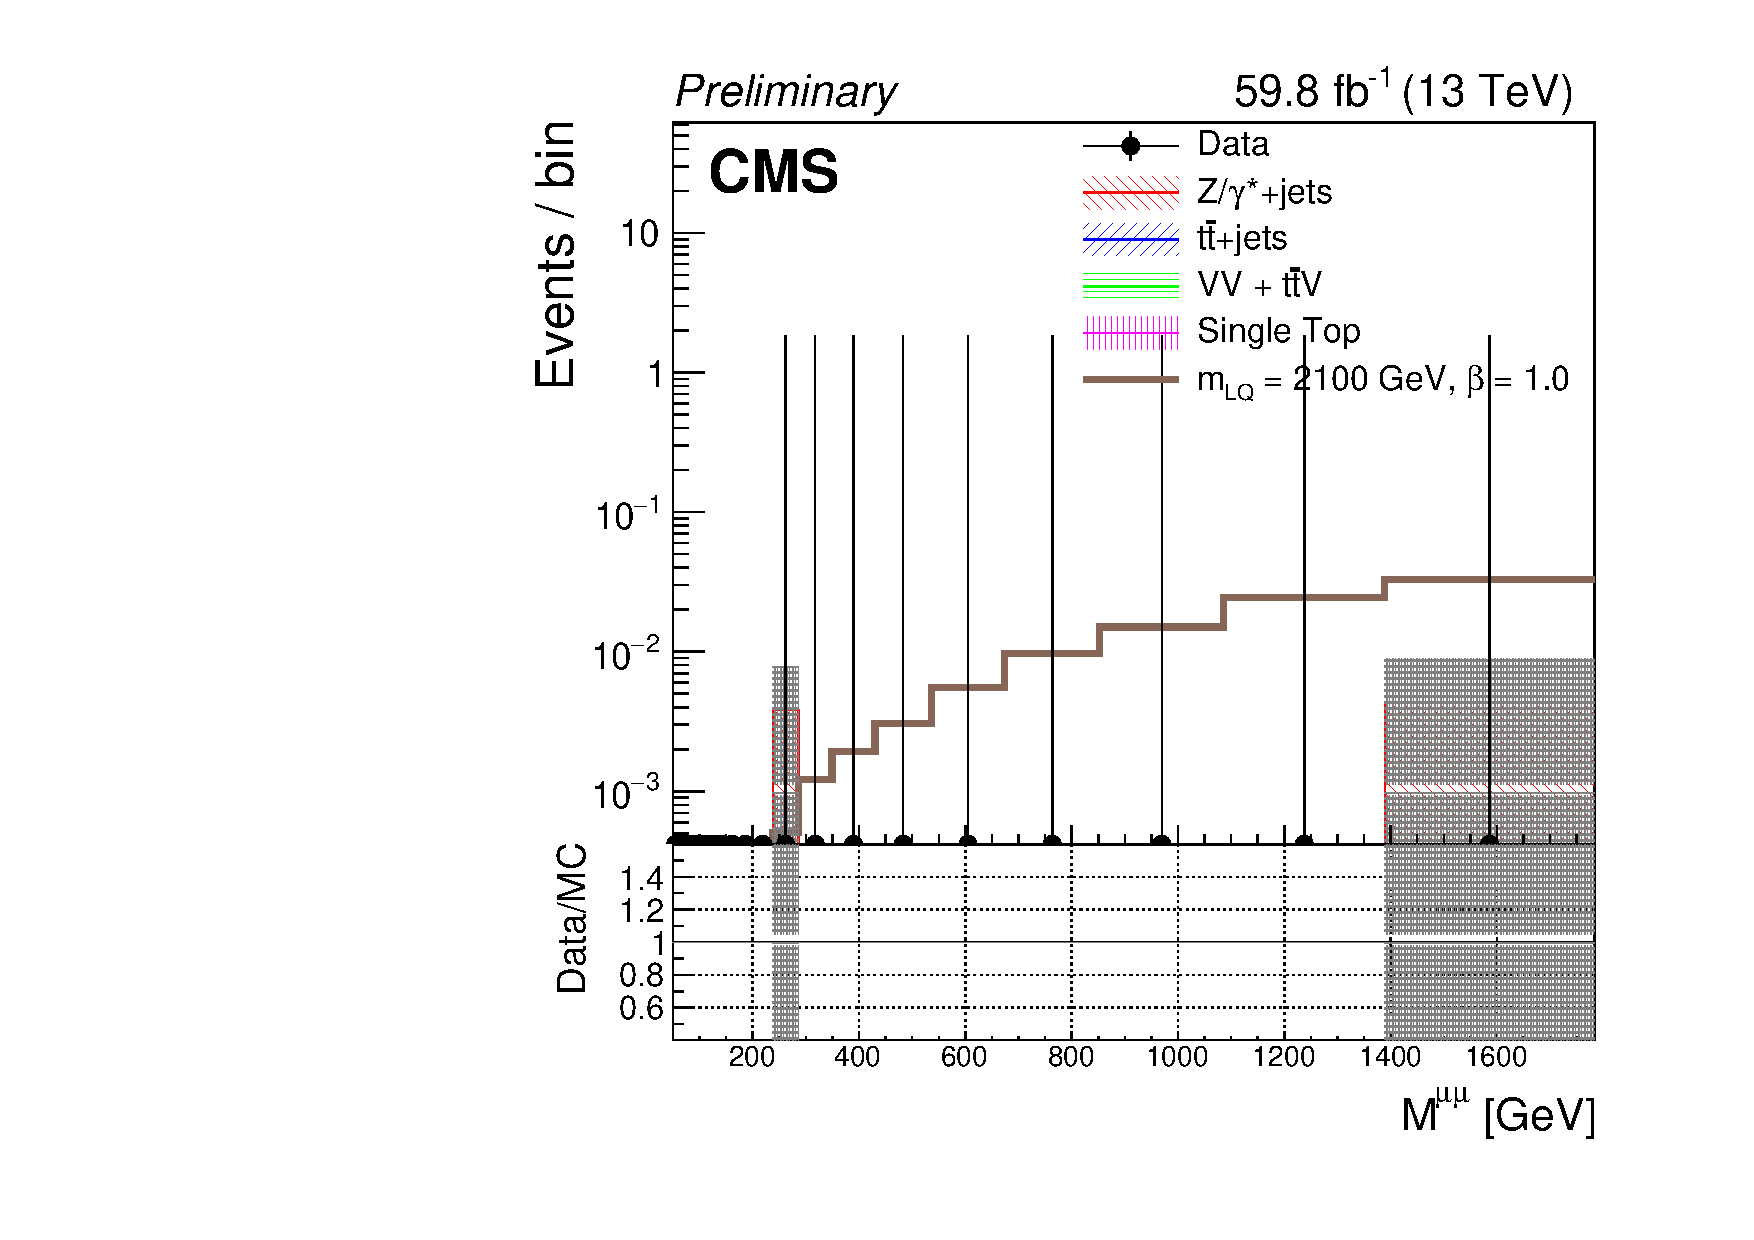
\includegraphics[width=.32\textwidth]{Images/Analysis/Results_2018_Unblinded/Plots/Final_selection/BasicLQ_uujj_M_uu_final2100.pdf}}
    \caption{BDT input variable \Muu at final selection in 2016 (left), 2017 (middle), and 2018 (right) simulation. Final selection cuts correspond to \SI{1500}{GeV} (top), \SI{1800}{GeV} (middle), and \SI{2100}{GeV} (bottom) leptoquark signal samples. Error bars represent statistical uncertainties, while the shaded area represents systematic uncertainties.
    \label{figapp:finalSelMuu}}
\end{figure}
\begin{figure}[H]
    \centering
    {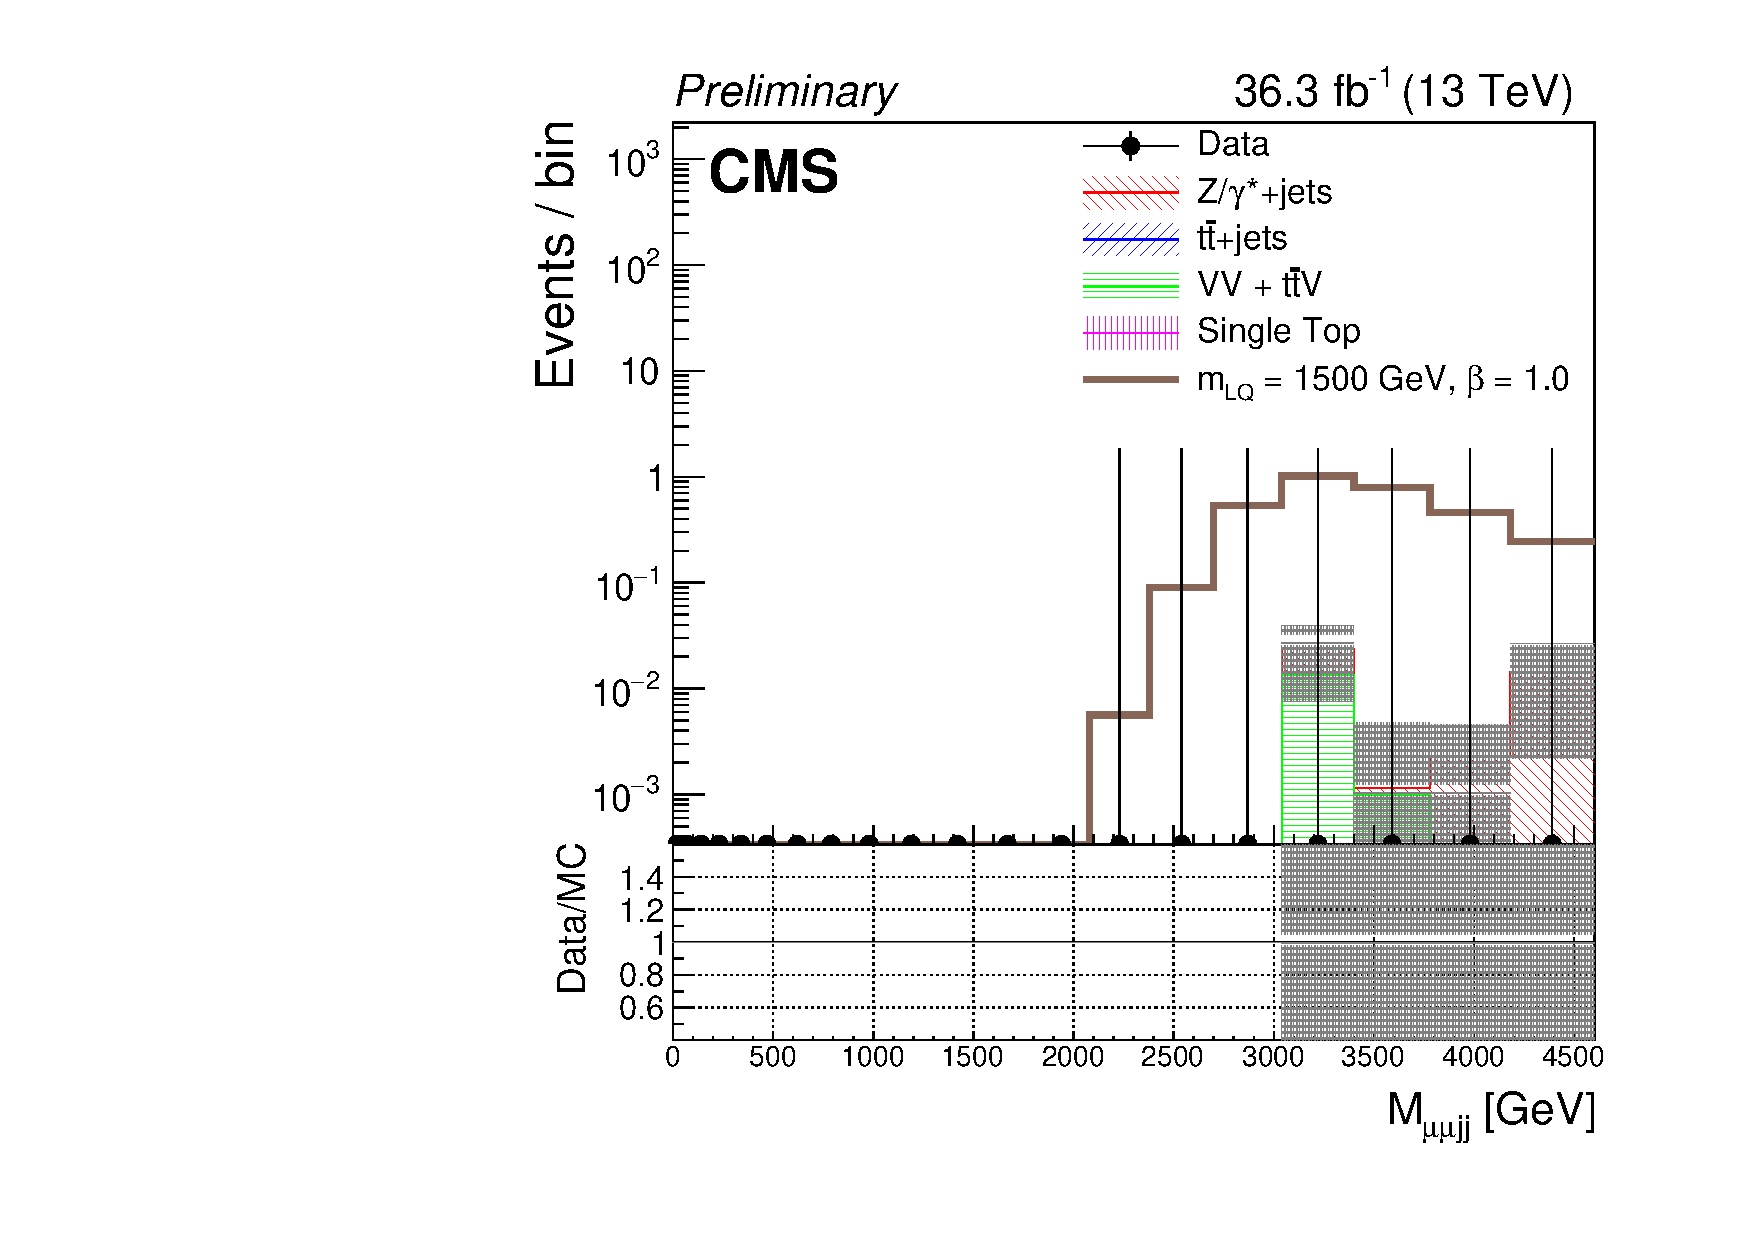
\includegraphics[width=.32\textwidth]{Images/Analysis/Results_2016_Unblinded/Plots/Final_selection/BasicLQ_uujj_M_uujj_final1500.pdf}}
    {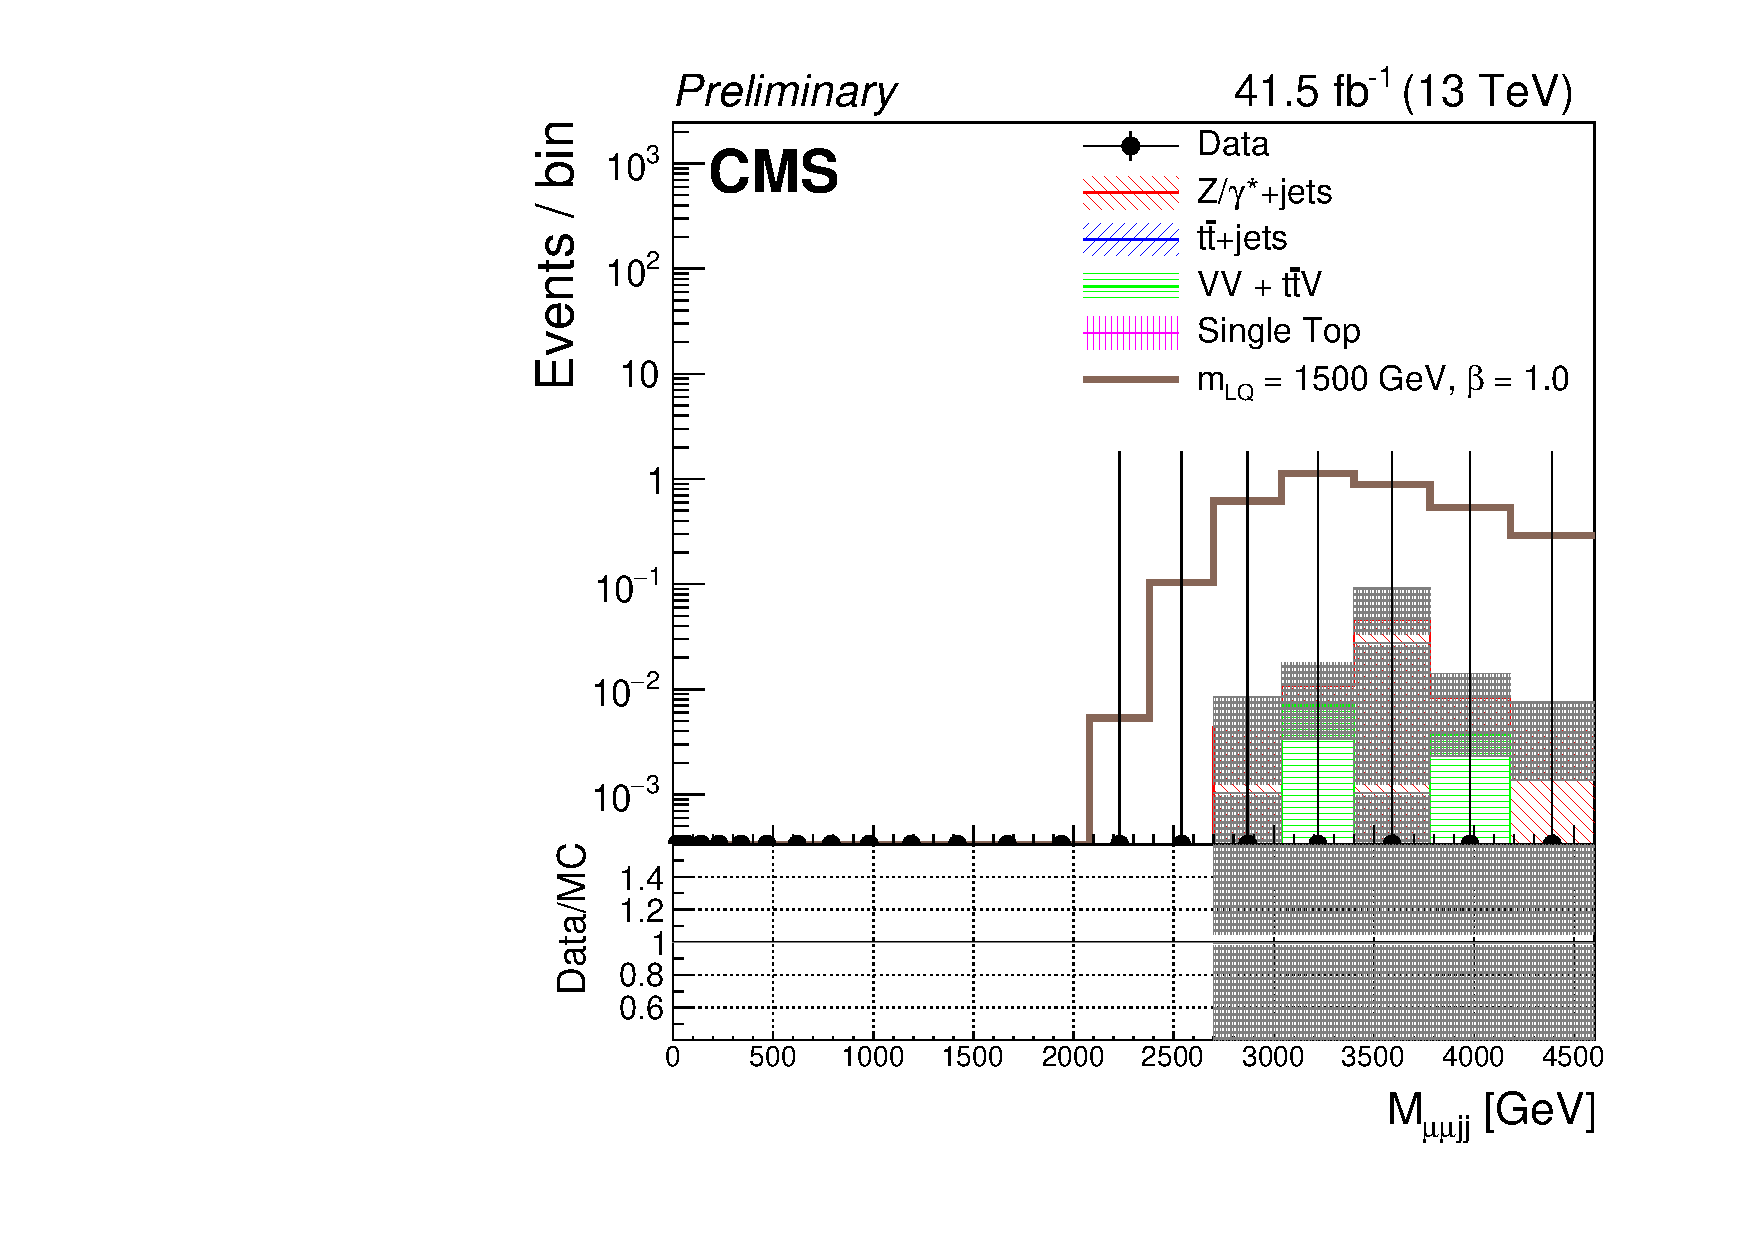
\includegraphics[width=.32\textwidth]{Images/Analysis/Results_2017_Unblinded/Plots/Final_selection/BasicLQ_uujj_M_uujj_final1500.pdf}}
    {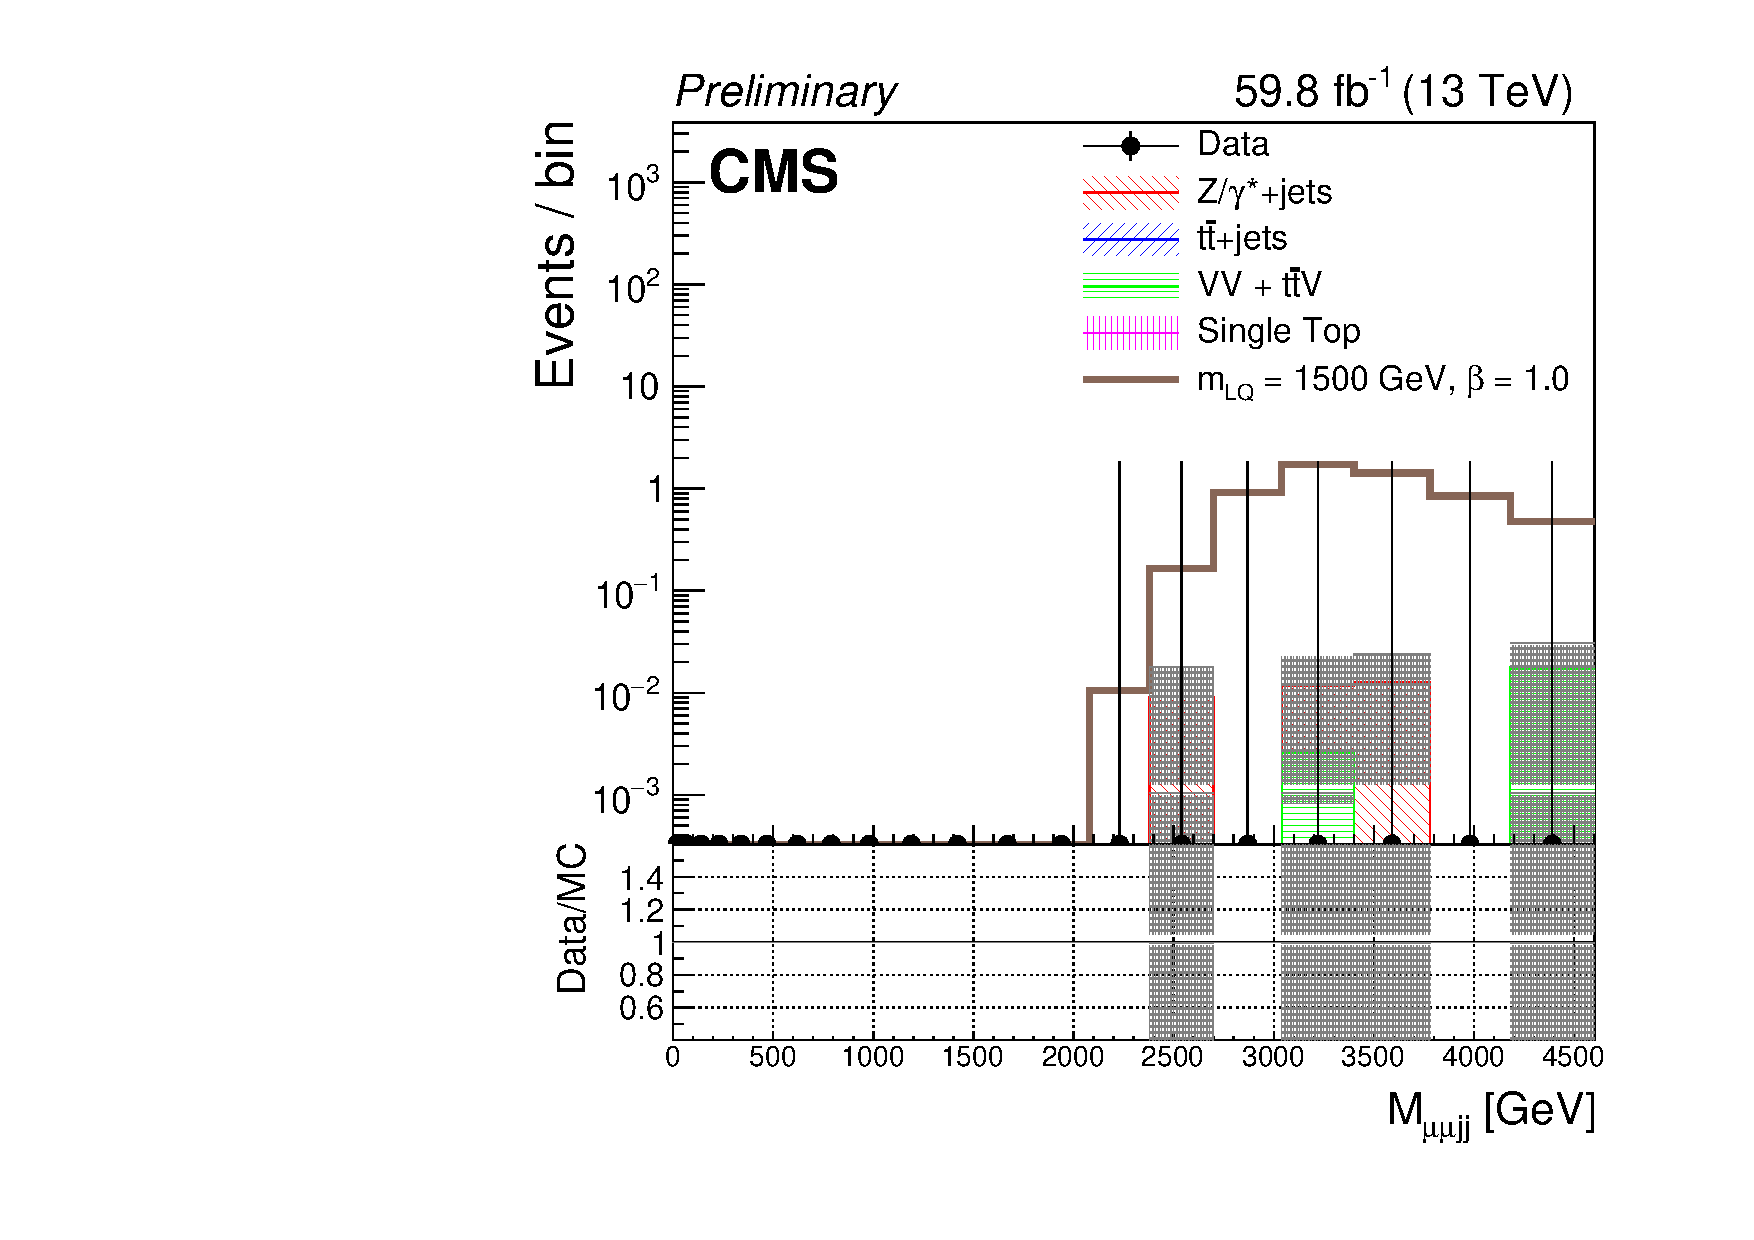
\includegraphics[width=.32\textwidth]{Images/Analysis/Results_2018_Unblinded/Plots/Final_selection/BasicLQ_uujj_M_uujj_final1500.pdf}}
    {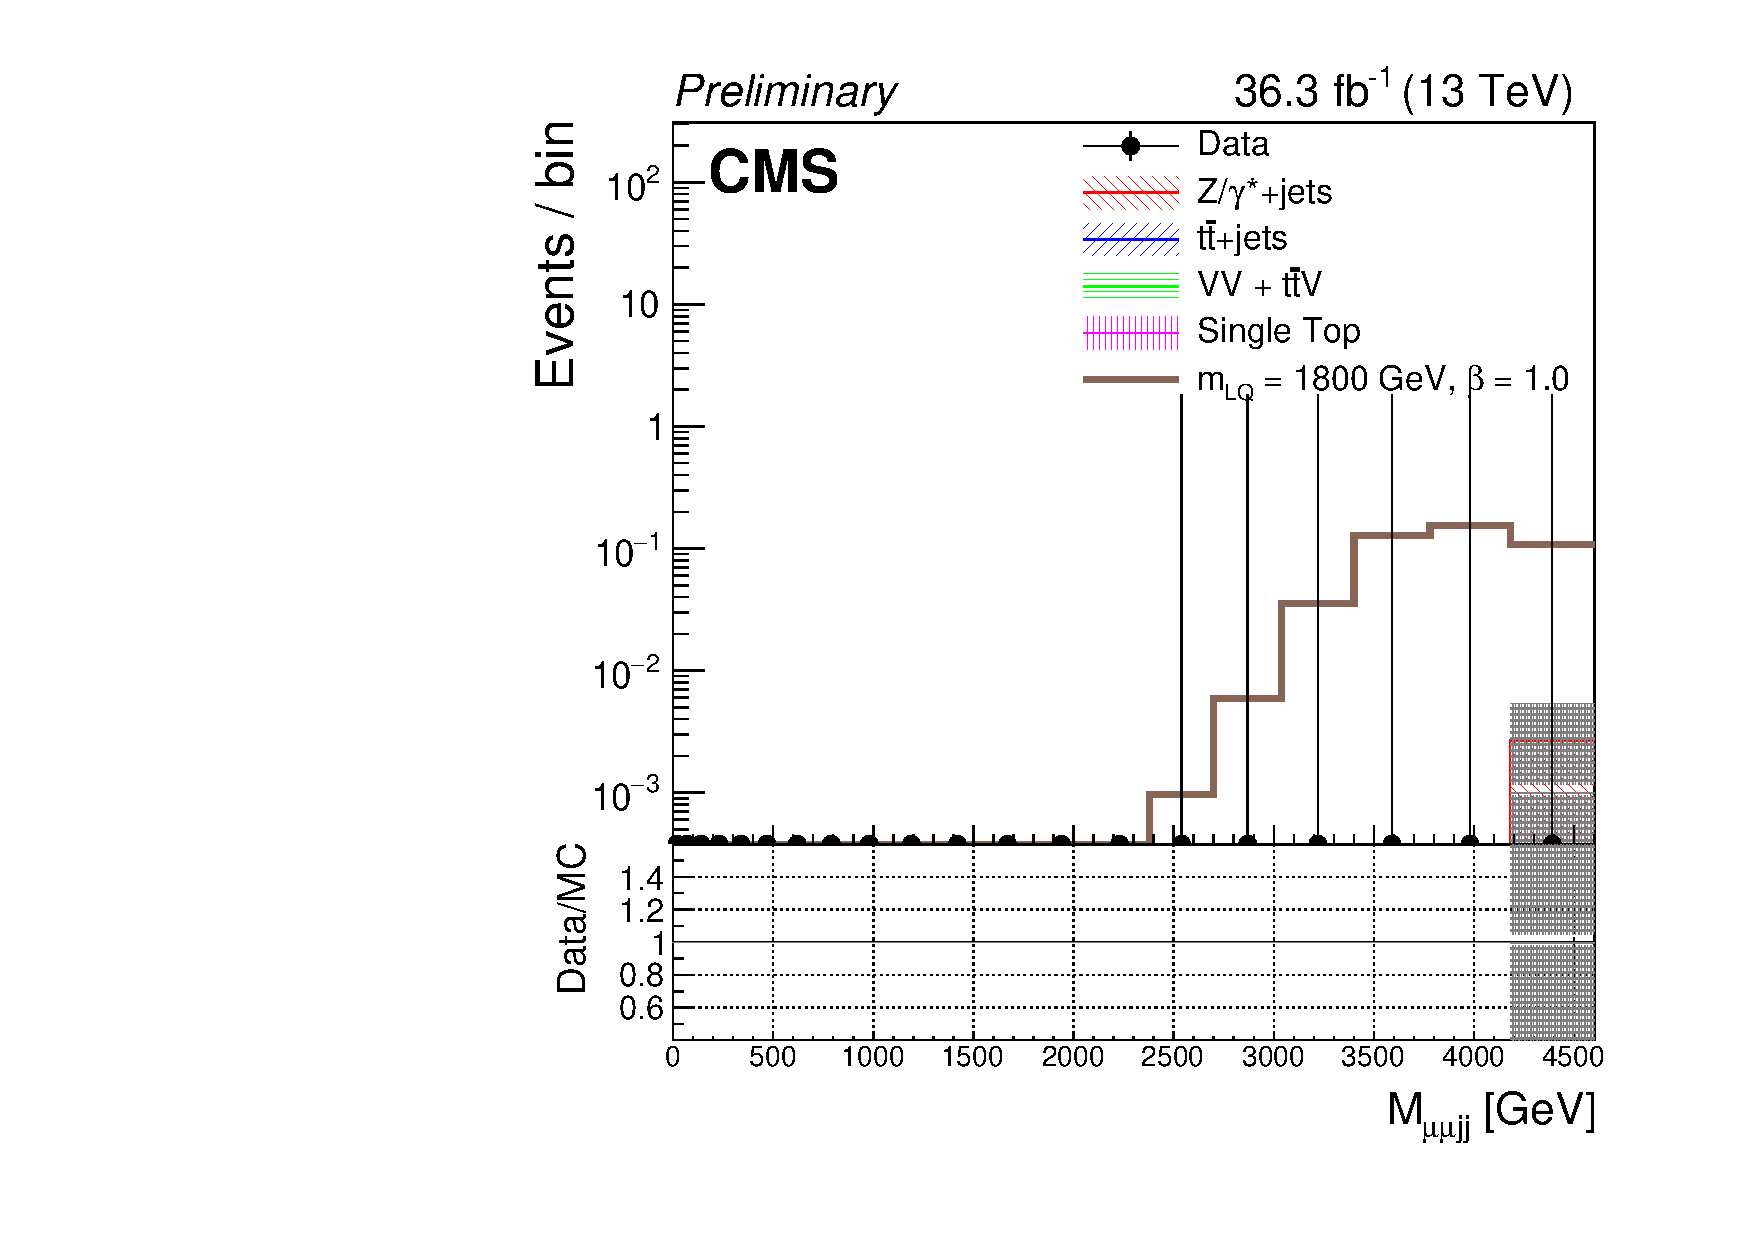
\includegraphics[width=.32\textwidth]{Images/Analysis/Results_2016_Unblinded/Plots/Final_selection/BasicLQ_uujj_M_uujj_final1800.pdf}}
    {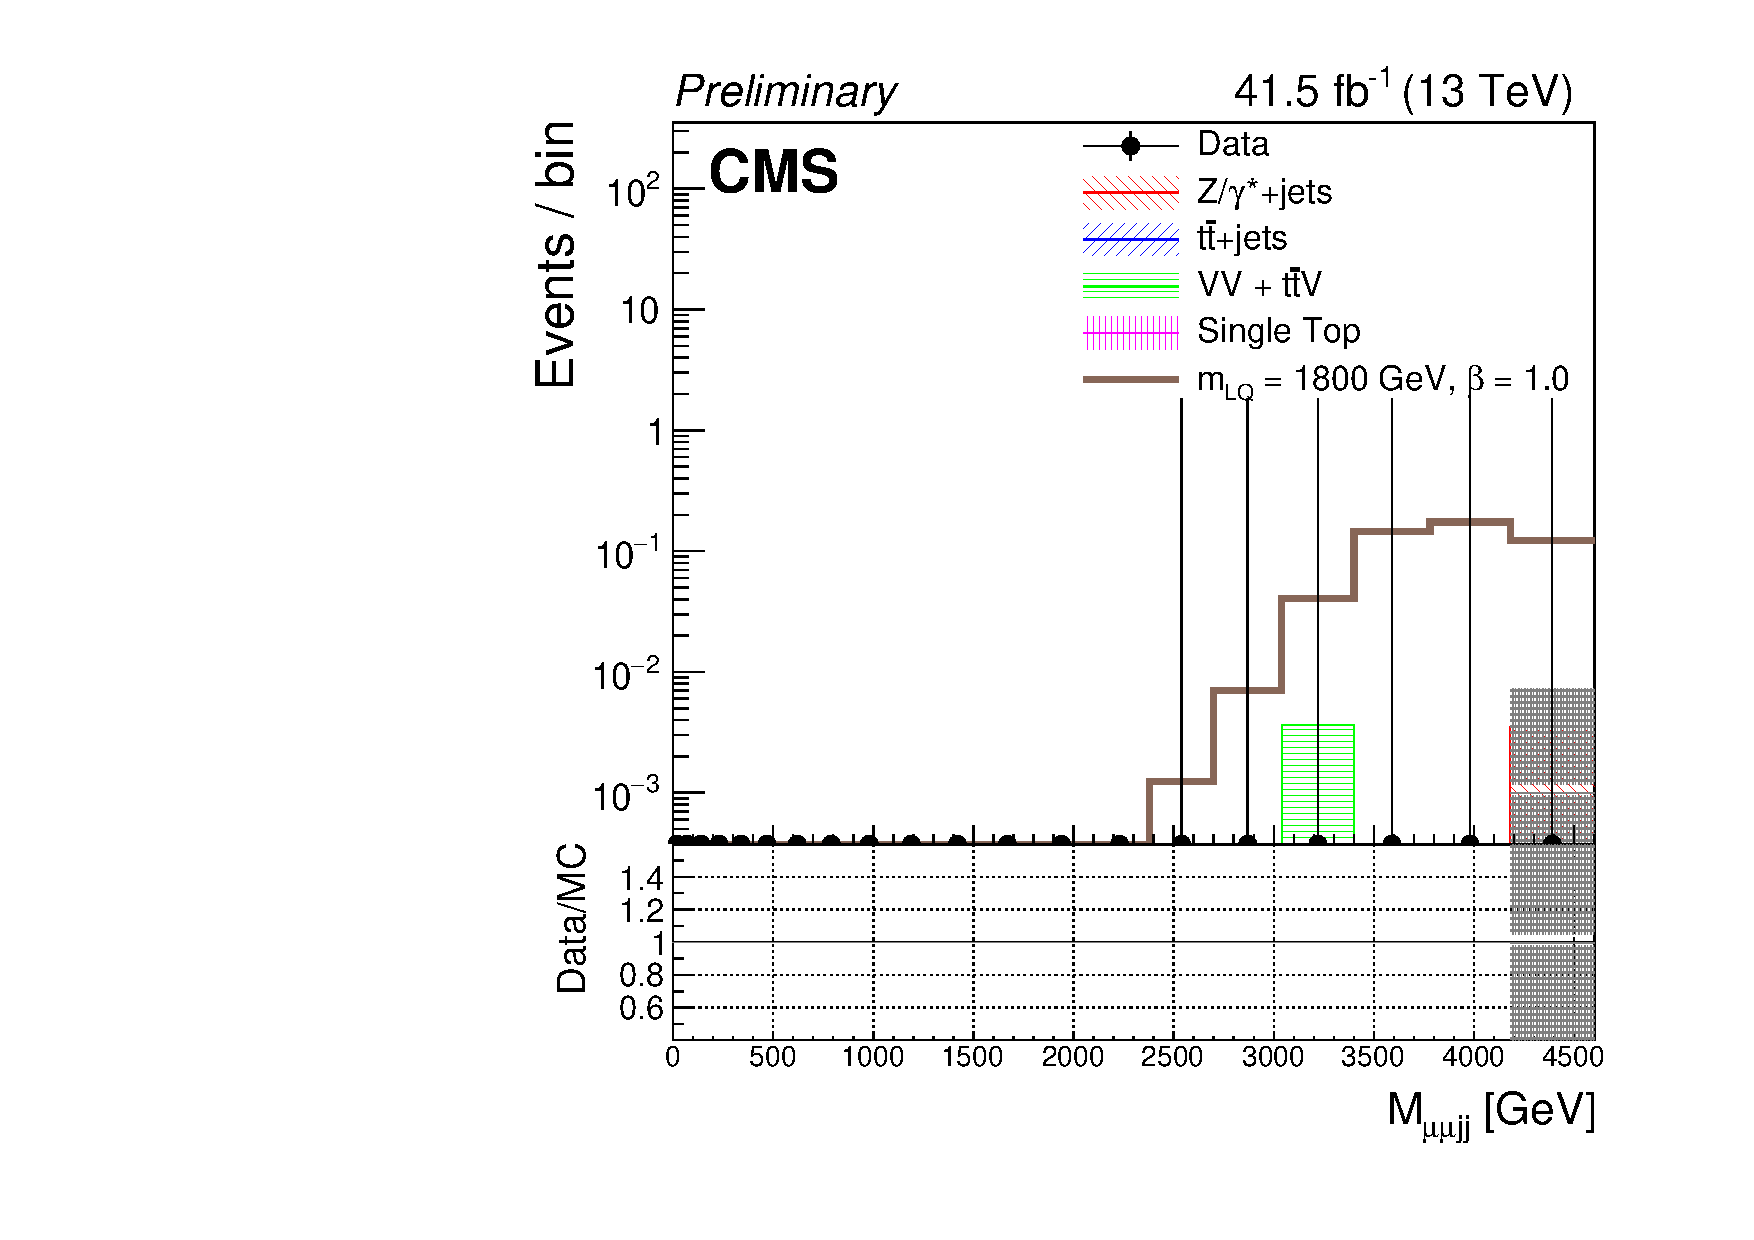
\includegraphics[width=.32\textwidth]{Images/Analysis/Results_2017_Unblinded/Plots/Final_selection/BasicLQ_uujj_M_uujj_final1800.pdf}}
    {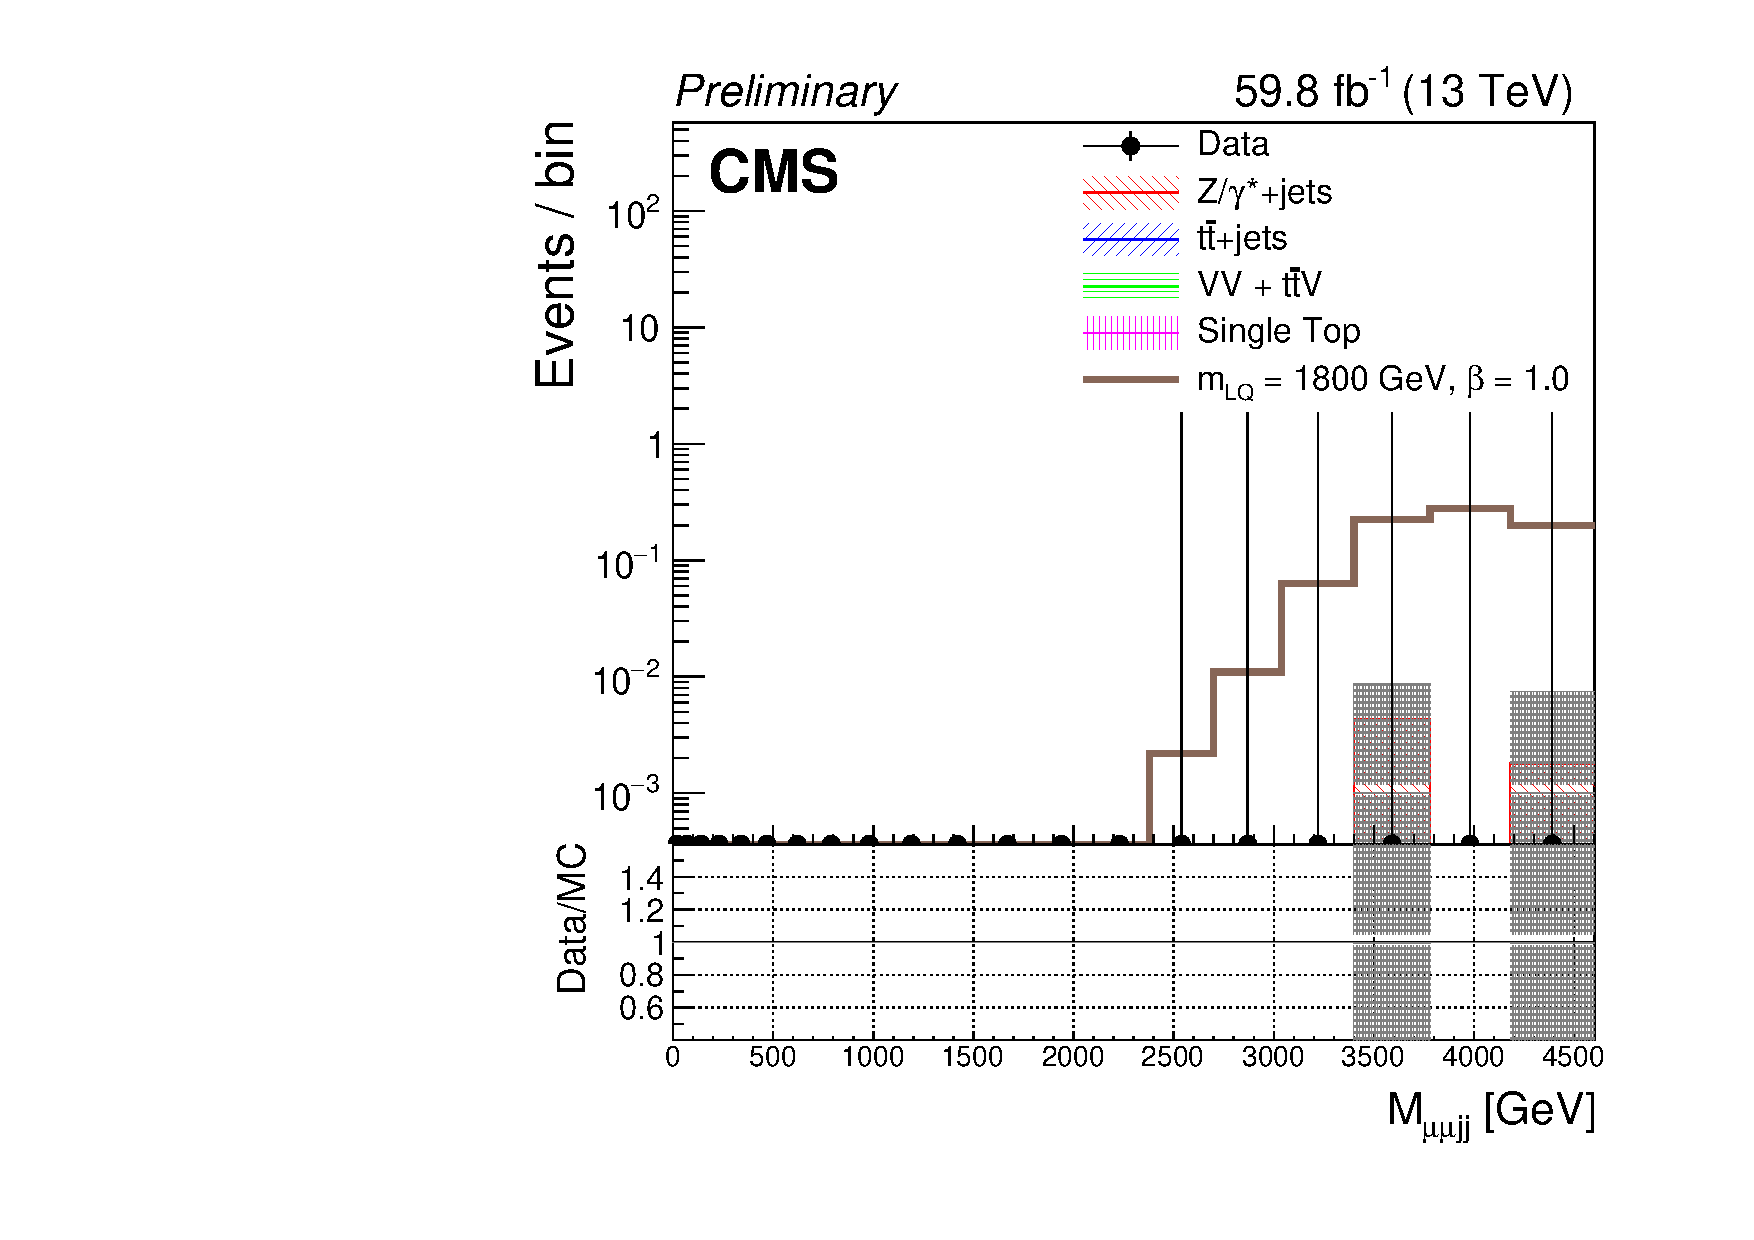
\includegraphics[width=.32\textwidth]{Images/Analysis/Results_2018_Unblinded/Plots/Final_selection/BasicLQ_uujj_M_uujj_final1800.pdf}}
    {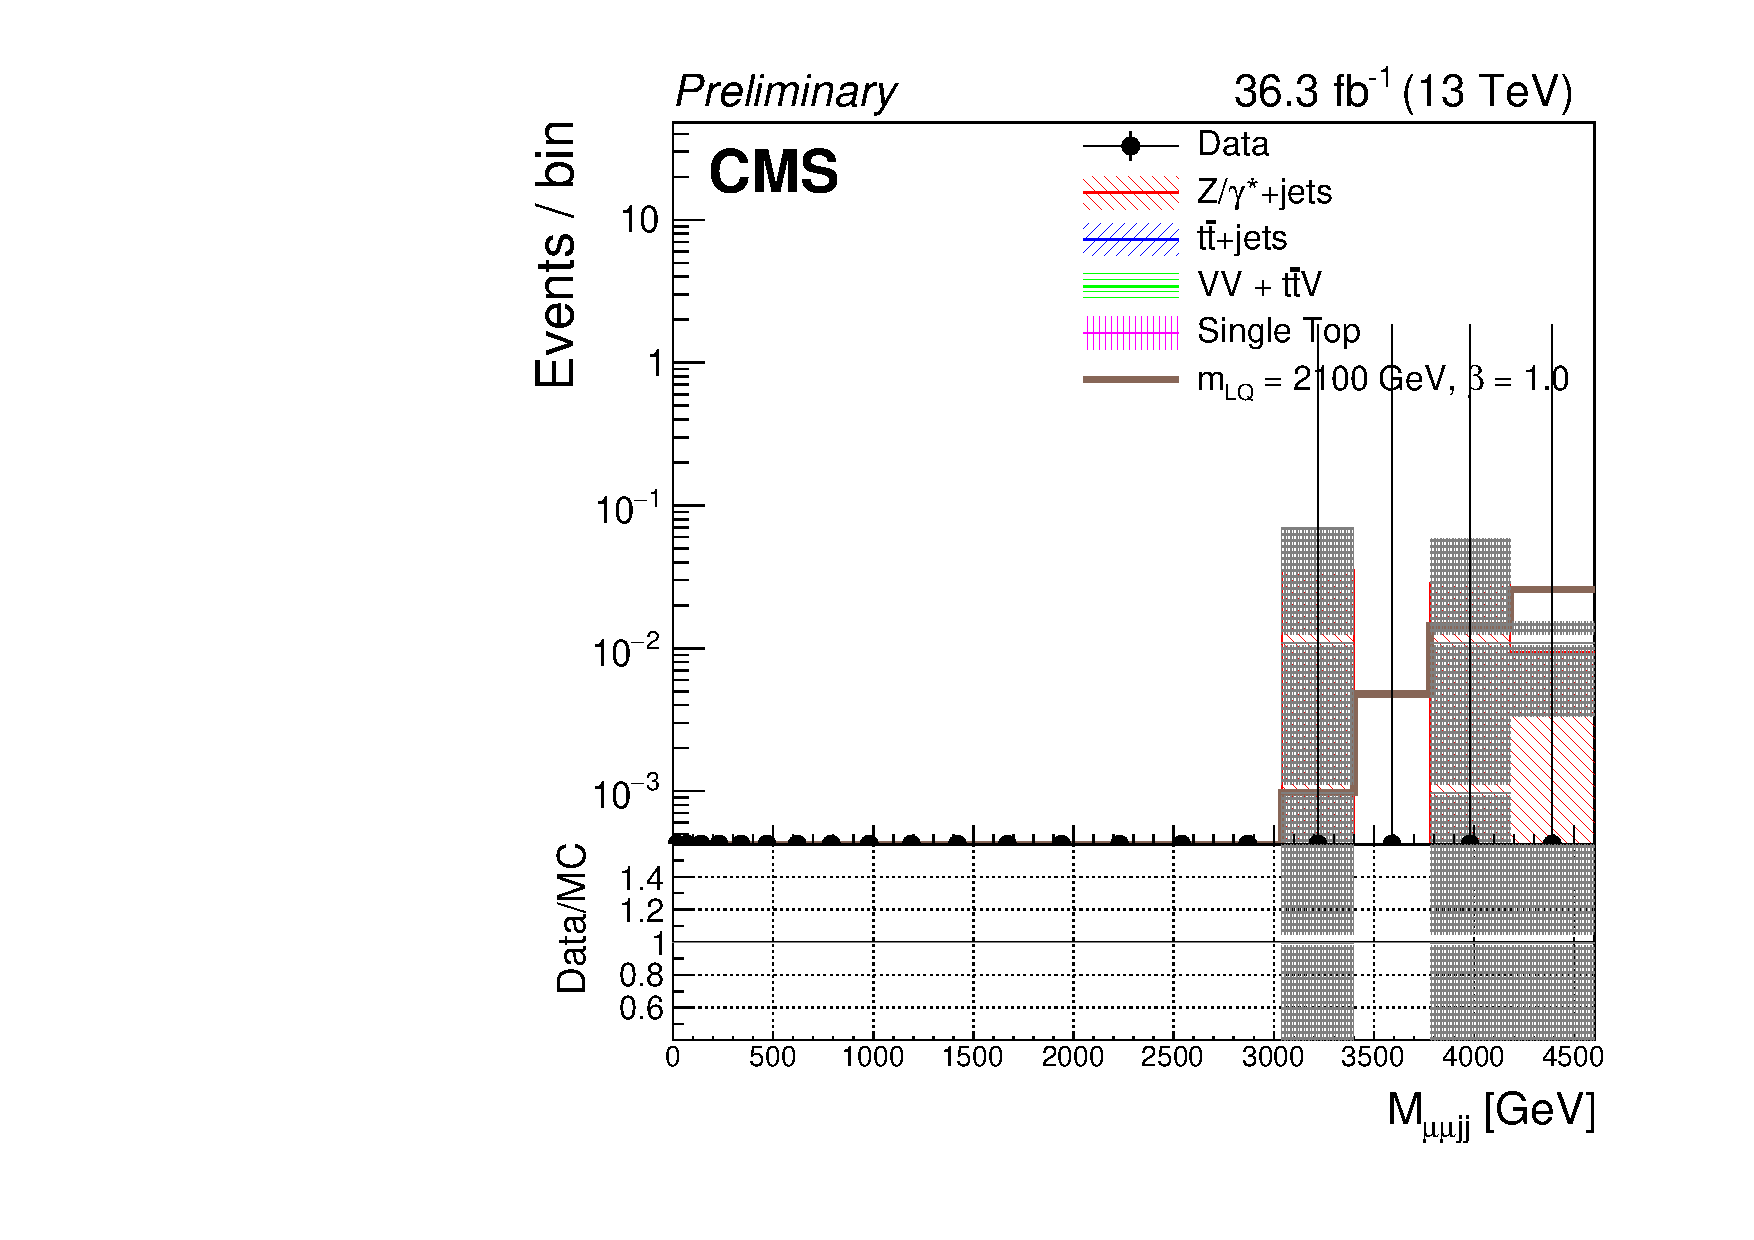
\includegraphics[width=.32\textwidth]{Images/Analysis/Results_2016_Unblinded/Plots/Final_selection/BasicLQ_uujj_M_uujj_final2100.pdf}}
    {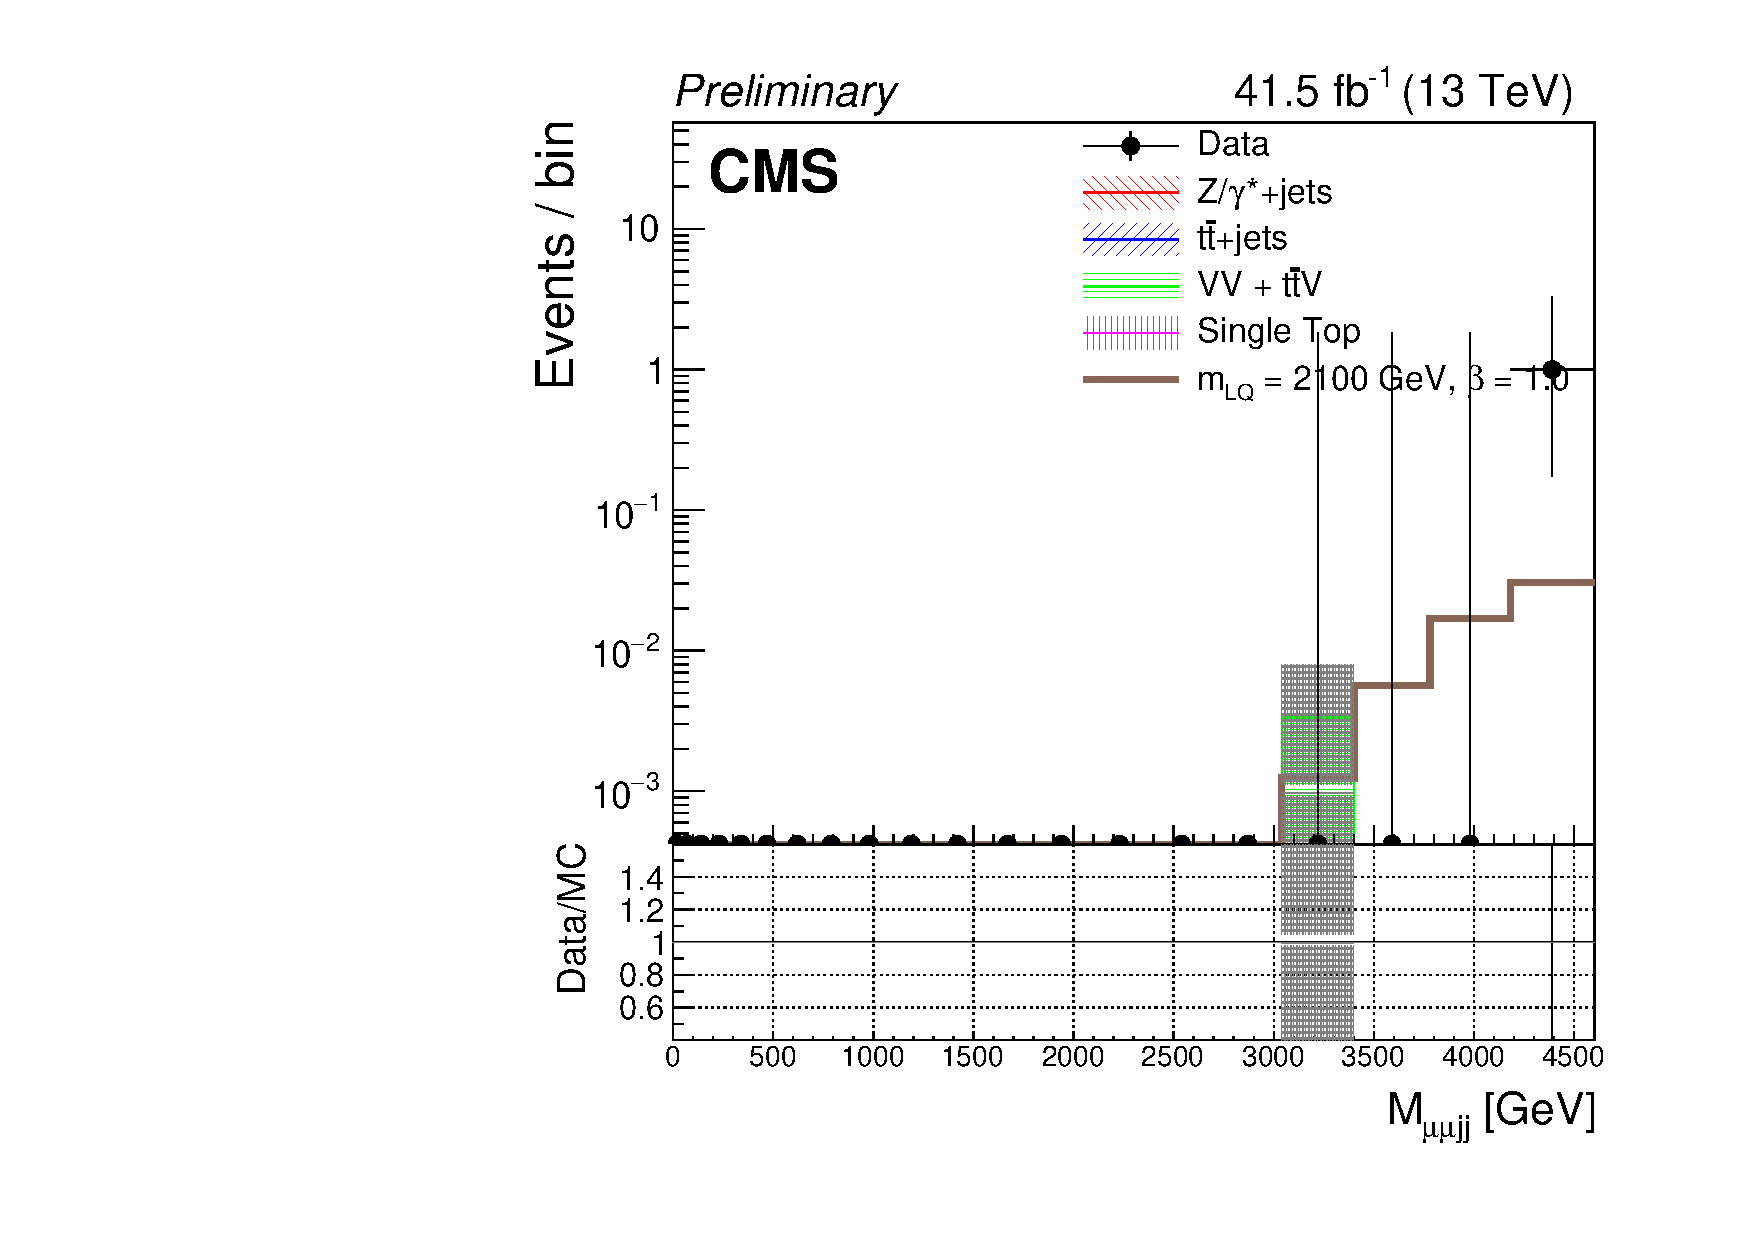
\includegraphics[width=.32\textwidth]{Images/Analysis/Results_2017_Unblinded/Plots/Final_selection/BasicLQ_uujj_M_uujj_final2100.pdf}}
    {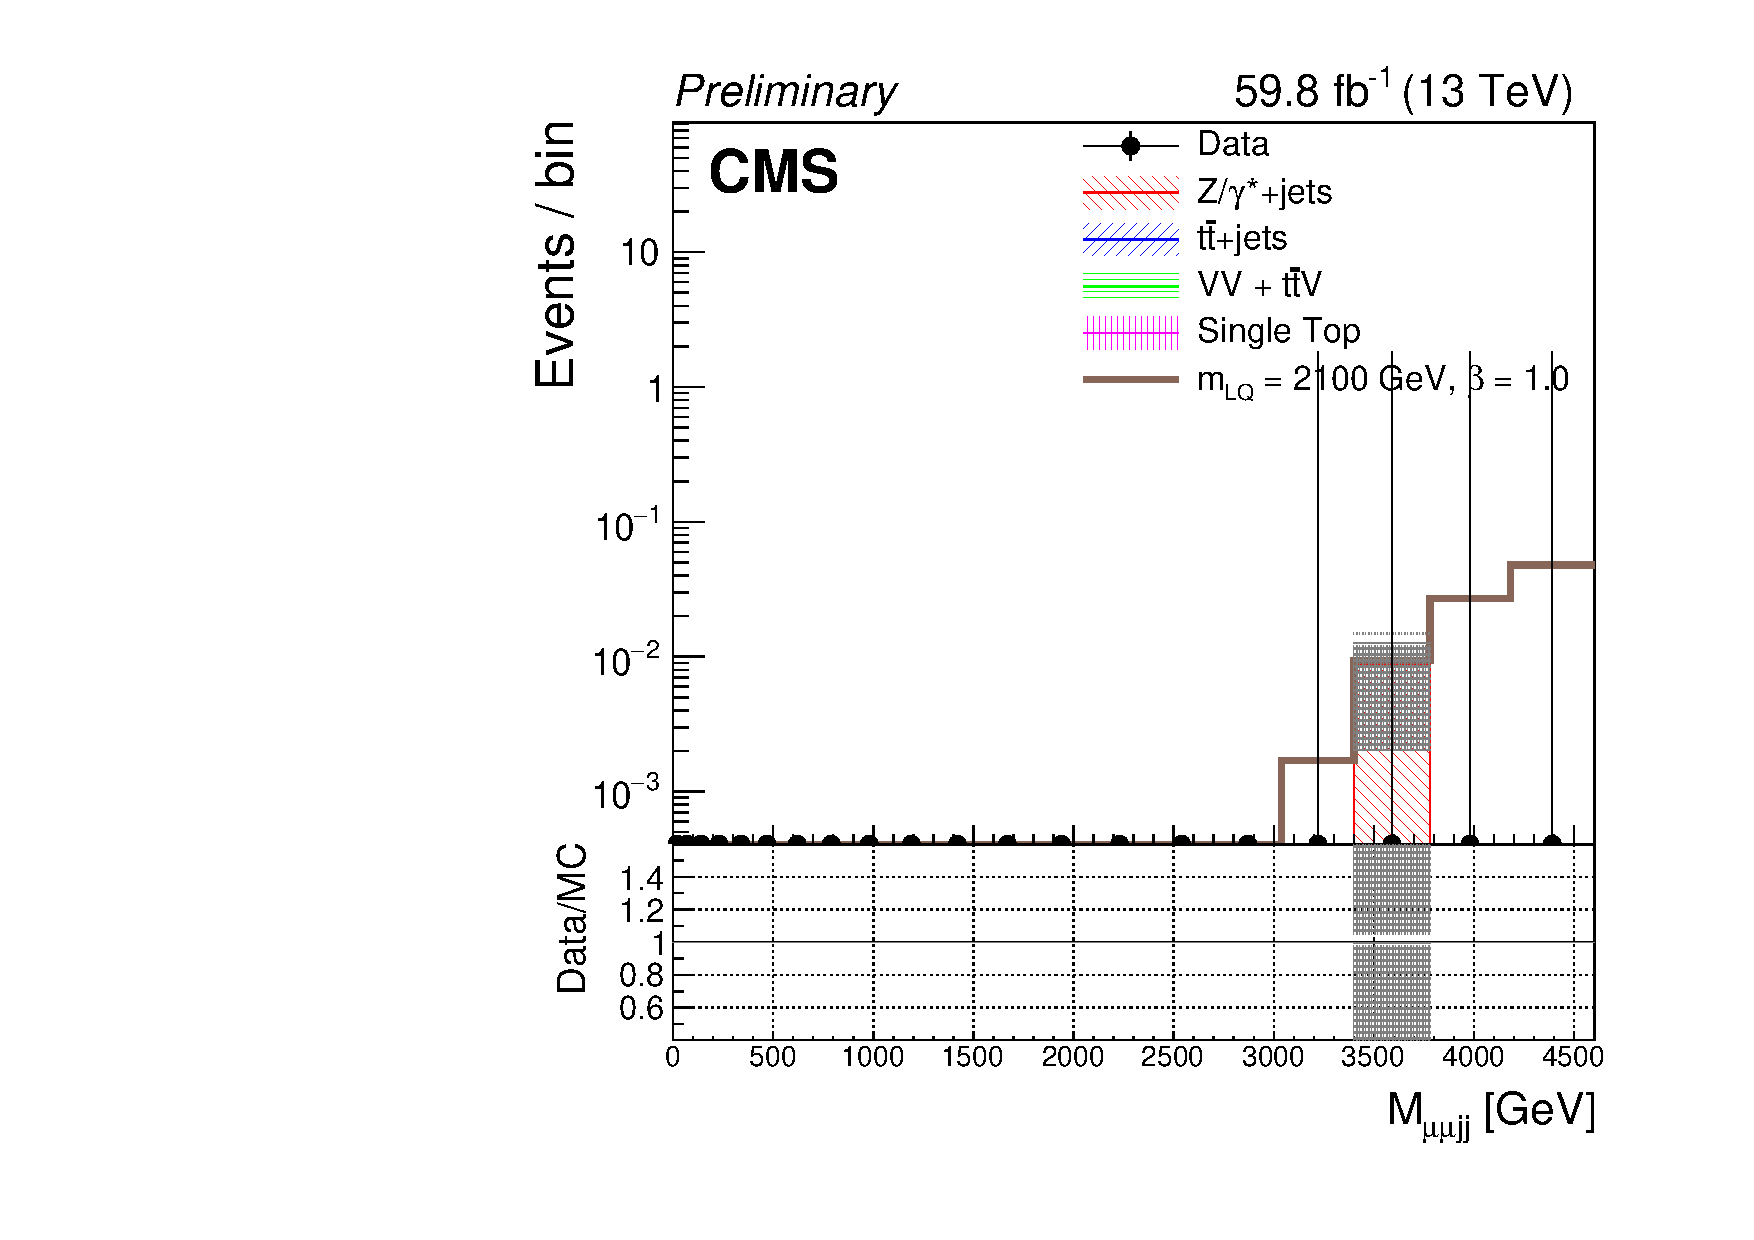
\includegraphics[width=.32\textwidth]{Images/Analysis/Results_2018_Unblinded/Plots/Final_selection/BasicLQ_uujj_M_uujj_final2100.pdf}}
    \caption{BDT input variable \Muujj at final selection in 2016 (left), 2017 (middle), and 2018 (right) simulation. Final selection cuts correspond to \SI{1500}{GeV} (top), \SI{1800}{GeV} (middle), and \SI{2100}{GeV} (bottom) leptoquark signal samples. Error bars represent statistical uncertainties, while the shaded area represents systematic uncertainties.
    \label{figapp:finalSelMuujj}}
\end{figure}
\begin{figure}[H]
    \centering
    {\includegraphics[width=.32\textwidth]{Images/Analysis/Results_2016_Unblinded/Plots/Final_selection/BasicLQ_uujj_M_uujj1_final1500.pdf}}
    {\includegraphics[width=.32\textwidth]{Images/Analysis/Results_2017_Unblinded/Plots/Final_selection/BasicLQ_uujj_M_uujj1_final1500.pdf}}
    {\includegraphics[width=.32\textwidth]{Images/Analysis/Results_2018_Unblinded/Plots/Final_selection/BasicLQ_uujj_M_uujj1_final1500.pdf}}
    {\includegraphics[width=.32\textwidth]{Images/Analysis/Results_2016_Unblinded/Plots/Final_selection/BasicLQ_uujj_M_uujj1_final1800.pdf}}
    {\includegraphics[width=.32\textwidth]{Images/Analysis/Results_2017_Unblinded/Plots/Final_selection/BasicLQ_uujj_M_uujj1_final1800.pdf}}
    {\includegraphics[width=.32\textwidth]{Images/Analysis/Results_2018_Unblinded/Plots/Final_selection/BasicLQ_uujj_M_uujj1_final1800.pdf}}
    {\includegraphics[width=.32\textwidth]{Images/Analysis/Results_2016_Unblinded/Plots/Final_selection/BasicLQ_uujj_M_uujj1_final2100.pdf}}
    {\includegraphics[width=.32\textwidth]{Images/Analysis/Results_2017_Unblinded/Plots/Final_selection/BasicLQ_uujj_M_uujj1_final2100.pdf}}
    {\includegraphics[width=.32\textwidth]{Images/Analysis/Results_2018_Unblinded/Plots/Final_selection/BasicLQ_uujj_M_uujj1_final2100.pdf}}
    \caption{BDT input variable \MujOne at final selection in 2016 (left), 2017 (middle), and 2018 (right) simulation. Final selection cuts correspond to \SI{1500}{GeV} (top), \SI{1800}{GeV} (middle), and \SI{2100}{GeV} (bottom) leptoquark signal samples. Error bars represent statistical uncertainties, while the shaded area represents systematic uncertainties.
    \label{figapp:finalSelMuujj1}}
\end{figure}
\begin{figure}[H]
    \centering
    {\includegraphics[width=.32\textwidth]{Images/Analysis/Results_2016_Unblinded/Plots/Final_selection/BasicLQ_uujj_M_uujj2_final1500.pdf}}
    {\includegraphics[width=.32\textwidth]{Images/Analysis/Results_2017_Unblinded/Plots/Final_selection/BasicLQ_uujj_M_uujj2_final1500.pdf}}
    {\includegraphics[width=.32\textwidth]{Images/Analysis/Results_2018_Unblinded/Plots/Final_selection/BasicLQ_uujj_M_uujj2_final1500.pdf}}
    {\includegraphics[width=.32\textwidth]{Images/Analysis/Results_2016_Unblinded/Plots/Final_selection/BasicLQ_uujj_M_uujj2_final1800.pdf}}
    {\includegraphics[width=.32\textwidth]{Images/Analysis/Results_2017_Unblinded/Plots/Final_selection/BasicLQ_uujj_M_uujj2_final1800.pdf}}
    {\includegraphics[width=.32\textwidth]{Images/Analysis/Results_2018_Unblinded/Plots/Final_selection/BasicLQ_uujj_M_uujj2_final1800.pdf}}
    {\includegraphics[width=.32\textwidth]{Images/Analysis/Results_2016_Unblinded/Plots/Final_selection/BasicLQ_uujj_M_uujj2_final2100.pdf}}
    {\includegraphics[width=.32\textwidth]{Images/Analysis/Results_2017_Unblinded/Plots/Final_selection/BasicLQ_uujj_M_uujj2_final2100.pdf}}
    {\includegraphics[width=.32\textwidth]{Images/Analysis/Results_2018_Unblinded/Plots/Final_selection/BasicLQ_uujj_M_uujj2_final2100.pdf}}
    \caption{BDT input variable \MujTwo at final selection in 2016 (left), 2017 (middle), and 2018 (right) simulation. Final selection cuts correspond to \SI{1500}{GeV} (top), \SI{1800}{GeV} (middle), and \SI{2100}{GeV} (bottom) leptoquark signal samples. Error bars represent statistical uncertainties, while the shaded area represents systematic uncertainties.
    \label{figapp:finalSelMuujj2}}
\end{figure}
\begin{figure}[H]
    \centering
    {\includegraphics[width=.32\textwidth]{Images/Analysis/Results_2016_Unblinded/Plots/Final_selection/BasicLQ_uujj_St_uujj_final1500.pdf}}
    {\includegraphics[width=.32\textwidth]{Images/Analysis/Results_2017_Unblinded/Plots/Final_selection/BasicLQ_uujj_St_uujj_final1500.pdf}}
    {\includegraphics[width=.32\textwidth]{Images/Analysis/Results_2018_Unblinded/Plots/Final_selection/BasicLQ_uujj_St_uujj_final1500.pdf}}
    {\includegraphics[width=.32\textwidth]{Images/Analysis/Results_2016_Unblinded/Plots/Final_selection/BasicLQ_uujj_St_uujj_final1800.pdf}}
    {\includegraphics[width=.32\textwidth]{Images/Analysis/Results_2017_Unblinded/Plots/Final_selection/BasicLQ_uujj_St_uujj_final1800.pdf}}
    {\includegraphics[width=.32\textwidth]{Images/Analysis/Results_2018_Unblinded/Plots/Final_selection/BasicLQ_uujj_St_uujj_final1800.pdf}}
    {\includegraphics[width=.32\textwidth]{Images/Analysis/Results_2016_Unblinded/Plots/Final_selection/BasicLQ_uujj_St_uujj_final2100.pdf}}
    {\includegraphics[width=.32\textwidth]{Images/Analysis/Results_2017_Unblinded/Plots/Final_selection/BasicLQ_uujj_St_uujj_final2100.pdf}}
    {\includegraphics[width=.32\textwidth]{Images/Analysis/Results_2018_Unblinded/Plots/Final_selection/BasicLQ_uujj_St_uujj_final2100.pdf}}
    \caption{BDT input variable \ST at final selection in 2016 (left), 2017 (middle), and 2018 (right) simulation. Final selection cuts correspond to \SI{1500}{GeV} (top), \SI{1800}{GeV} (middle), and \SI{2100}{GeV} (bottom) leptoquark signal samples. Error bars represent statistical uncertainties, while the shaded area represents systematic uncertainties.
    \label{figapp:finalSelST}}
\end{figure}
\begin{figure}[H]
    \centering
    {\includegraphics[width=.32\textwidth]{Images/Analysis/Results_2016_Unblinded/Plots/Final_selection/BasicLQ_uujj_Pt_miss_final1500.pdf}}
    {\includegraphics[width=.32\textwidth]{Images/Analysis/Results_2017_Unblinded/Plots/Final_selection/BasicLQ_uujj_Pt_miss_final1500.pdf}}
    {\includegraphics[width=.32\textwidth]{Images/Analysis/Results_2018_Unblinded/Plots/Final_selection/BasicLQ_uujj_Pt_miss_final1500.pdf}}
    {\includegraphics[width=.32\textwidth]{Images/Analysis/Results_2016_Unblinded/Plots/Final_selection/BasicLQ_uujj_Pt_miss_final1800.pdf}}
    {\includegraphics[width=.32\textwidth]{Images/Analysis/Results_2017_Unblinded/Plots/Final_selection/BasicLQ_uujj_Pt_miss_final1800.pdf}}
    {\includegraphics[width=.32\textwidth]{Images/Analysis/Results_2018_Unblinded/Plots/Final_selection/BasicLQ_uujj_Pt_miss_final1800.pdf}}
    {\includegraphics[width=.32\textwidth]{Images/Analysis/Results_2016_Unblinded/Plots/Final_selection/BasicLQ_uujj_Pt_miss_final2100.pdf}}
    {\includegraphics[width=.32\textwidth]{Images/Analysis/Results_2017_Unblinded/Plots/Final_selection/BasicLQ_uujj_Pt_miss_final2100.pdf}}
    {\includegraphics[width=.32\textwidth]{Images/Analysis/Results_2018_Unblinded/Plots/Final_selection/BasicLQ_uujj_Pt_miss_final2100.pdf}}
    \caption{BDT input variable \ptmiss at final selection in 2016 (left), 2017 (middle), and 2018 (right) simulation. Final selection cuts correspond to \SI{1500}{GeV} (top), \SI{1800}{GeV} (middle), and \SI{2100}{GeV} (bottom) leptoquark signal samples. Error bars represent statistical uncertainties, while the shaded area represents systematic uncertainties.
    \label{figapp:finalSelMET}}
\end{figure}
\begin{figure}[H]
    \centering
    {\includegraphics[width=.32\textwidth]{Images/Analysis/Results_2016_Unblinded/Plots/Final_selection/BasicLQ_uujj_Pt_muon1_final1500.pdf}}
    {\includegraphics[width=.32\textwidth]{Images/Analysis/Results_2017_Unblinded/Plots/Final_selection/BasicLQ_uujj_Pt_muon1_final1500.pdf}}
    {\includegraphics[width=.32\textwidth]{Images/Analysis/Results_2018_Unblinded/Plots/Final_selection/BasicLQ_uujj_Pt_muon1_final1500.pdf}}
    {\includegraphics[width=.32\textwidth]{Images/Analysis/Results_2016_Unblinded/Plots/Final_selection/BasicLQ_uujj_Pt_muon1_final1800.pdf}}
    {\includegraphics[width=.32\textwidth]{Images/Analysis/Results_2017_Unblinded/Plots/Final_selection/BasicLQ_uujj_Pt_muon1_final1800.pdf}}
    {\includegraphics[width=.32\textwidth]{Images/Analysis/Results_2018_Unblinded/Plots/Final_selection/BasicLQ_uujj_Pt_muon1_final1800.pdf}}
    {\includegraphics[width=.32\textwidth]{Images/Analysis/Results_2016_Unblinded/Plots/Final_selection/BasicLQ_uujj_Pt_muon1_final2100.pdf}}
    {\includegraphics[width=.32\textwidth]{Images/Analysis/Results_2017_Unblinded/Plots/Final_selection/BasicLQ_uujj_Pt_muon1_final2100.pdf}}
    {\includegraphics[width=.32\textwidth]{Images/Analysis/Results_2018_Unblinded/Plots/Final_selection/BasicLQ_uujj_Pt_muon1_final2100.pdf}}
    \caption{BDT input variable \ptof{\PmuOne} at final selection in 2016 (left), 2017 (middle), and 2018 (right) simulation. Final selection cuts correspond to \SI{1500}{GeV} (top), \SI{1800}{GeV} (middle), and \SI{2100}{GeV} (bottom) leptoquark signal samples. Error bars represent statistical uncertainties, while the shaded area represents systematic uncertainties.
    \label{figapp:finalSelptu1}}
\end{figure}
\begin{figure}[H]
    \centering
    {\includegraphics[width=.32\textwidth]{Images/Analysis/Results_2016_Unblinded/Plots/Final_selection/BasicLQ_uujj_Pt_muon2_final1500.pdf}}
    {\includegraphics[width=.32\textwidth]{Images/Analysis/Results_2017_Unblinded/Plots/Final_selection/BasicLQ_uujj_Pt_muon2_final1500.pdf}}
    {\includegraphics[width=.32\textwidth]{Images/Analysis/Results_2018_Unblinded/Plots/Final_selection/BasicLQ_uujj_Pt_muon2_final1500.pdf}}
    {\includegraphics[width=.32\textwidth]{Images/Analysis/Results_2016_Unblinded/Plots/Final_selection/BasicLQ_uujj_Pt_muon2_final1800.pdf}}
    {\includegraphics[width=.32\textwidth]{Images/Analysis/Results_2017_Unblinded/Plots/Final_selection/BasicLQ_uujj_Pt_muon2_final1800.pdf}}
    {\includegraphics[width=.32\textwidth]{Images/Analysis/Results_2018_Unblinded/Plots/Final_selection/BasicLQ_uujj_Pt_muon2_final1800.pdf}}
    {\includegraphics[width=.32\textwidth]{Images/Analysis/Results_2016_Unblinded/Plots/Final_selection/BasicLQ_uujj_Pt_muon2_final2100.pdf}}
    {\includegraphics[width=.32\textwidth]{Images/Analysis/Results_2017_Unblinded/Plots/Final_selection/BasicLQ_uujj_Pt_muon2_final2100.pdf}}
    {\includegraphics[width=.32\textwidth]{Images/Analysis/Results_2018_Unblinded/Plots/Final_selection/BasicLQ_uujj_Pt_muon2_final2100.pdf}}
    \caption{BDT input variable \ptof{\PmuTwo} at final selection in 2016 (left), 2017 (middle), and 2018 (right) simulation. Final selection cuts correspond to \SI{1500}{GeV} (top), \SI{1800}{GeV} (middle), and \SI{2100}{GeV} (bottom) leptoquark signal samples. Error bars represent statistical uncertainties, while the shaded area represents systematic uncertainties.
    \label{figapp:finalSelptu2}}
\end{figure}
\begin{figure}[H]
    \centering
    {\includegraphics[width=.32\textwidth]{Images/Analysis/Results_2016_Unblinded/Plots/Final_selection/BasicLQ_uujj_Pt_jet1_final1500.pdf}}
    {\includegraphics[width=.32\textwidth]{Images/Analysis/Results_2017_Unblinded/Plots/Final_selection/BasicLQ_uujj_Pt_jet1_final1500.pdf}}
    {\includegraphics[width=.32\textwidth]{Images/Analysis/Results_2018_Unblinded/Plots/Final_selection/BasicLQ_uujj_Pt_jet1_final1500.pdf}}
    {\includegraphics[width=.32\textwidth]{Images/Analysis/Results_2016_Unblinded/Plots/Final_selection/BasicLQ_uujj_Pt_jet1_final1800.pdf}}
    {\includegraphics[width=.32\textwidth]{Images/Analysis/Results_2017_Unblinded/Plots/Final_selection/BasicLQ_uujj_Pt_jet1_final1800.pdf}}
    {\includegraphics[width=.32\textwidth]{Images/Analysis/Results_2018_Unblinded/Plots/Final_selection/BasicLQ_uujj_Pt_jet1_final1800.pdf}}
    {\includegraphics[width=.32\textwidth]{Images/Analysis/Results_2016_Unblinded/Plots/Final_selection/BasicLQ_uujj_Pt_jet1_final2100.pdf}}
    {\includegraphics[width=.32\textwidth]{Images/Analysis/Results_2017_Unblinded/Plots/Final_selection/BasicLQ_uujj_Pt_jet1_final2100.pdf}}
    {\includegraphics[width=.32\textwidth]{Images/Analysis/Results_2018_Unblinded/Plots/Final_selection/BasicLQ_uujj_Pt_jet1_final2100.pdf}}
    \caption{BDT input variable \ptof{\jetOne} at final selection in 2016 (left), 2017 (middle), and 2018 (right) simulation. Final selection cuts correspond to \SI{1500}{GeV} (top), \SI{1800}{GeV} (middle), and \SI{2100}{GeV} (bottom) leptoquark signal samples. Error bars represent statistical uncertainties, while the shaded area represents systematic uncertainties.
    \label{figapp:finalSelptj1}}
\end{figure}
\begin{figure}[H]
    \centering
    {\includegraphics[width=.32\textwidth]{Images/Analysis/Results_2016_Unblinded/Plots/Final_selection/BasicLQ_uujj_Pt_jet2_final1500.pdf}}
    {\includegraphics[width=.32\textwidth]{Images/Analysis/Results_2017_Unblinded/Plots/Final_selection/BasicLQ_uujj_Pt_jet2_final1500.pdf}}
    {\includegraphics[width=.32\textwidth]{Images/Analysis/Results_2018_Unblinded/Plots/Final_selection/BasicLQ_uujj_Pt_jet2_final1500.pdf}}
    {\includegraphics[width=.32\textwidth]{Images/Analysis/Results_2016_Unblinded/Plots/Final_selection/BasicLQ_uujj_Pt_jet2_final1800.pdf}}
    {\includegraphics[width=.32\textwidth]{Images/Analysis/Results_2017_Unblinded/Plots/Final_selection/BasicLQ_uujj_Pt_jet2_final1800.pdf}}
    {\includegraphics[width=.32\textwidth]{Images/Analysis/Results_2018_Unblinded/Plots/Final_selection/BasicLQ_uujj_Pt_jet2_final1800.pdf}}
    {\includegraphics[width=.32\textwidth]{Images/Analysis/Results_2016_Unblinded/Plots/Final_selection/BasicLQ_uujj_Pt_jet2_final2100.pdf}}
    {\includegraphics[width=.32\textwidth]{Images/Analysis/Results_2017_Unblinded/Plots/Final_selection/BasicLQ_uujj_Pt_jet2_final2100.pdf}}
    {\includegraphics[width=.32\textwidth]{Images/Analysis/Results_2018_Unblinded/Plots/Final_selection/BasicLQ_uujj_Pt_jet2_final2100.pdf}}
    \caption{BDT input variable \ptof{\jetTwo} at final selection in 2016 (left), 2017 (middle), and 2018 (right) simulation. Final selection cuts correspond to \SI{1500}{GeV} (top), \SI{1800}{GeV} (middle), and \SI{2100}{GeV} (bottom) leptoquark signal samples. Error bars represent statistical uncertainties, while the shaded area represents systematic uncertainties.
    \label{figapp:finalSelptj2}}
\end{figure}
\begin{figure}[H]
    \centering
    {\includegraphics[width=.32\textwidth]{Images/Analysis/Results_2016_Unblinded/Plots/Final_selection/BasicLQ_uujj_DR_dimuonjet1_final1500.pdf}}
    {\includegraphics[width=.32\textwidth]{Images/Analysis/Results_2017_Unblinded/Plots/Final_selection/BasicLQ_uujj_DR_dimuonjet1_final1500.pdf}}
    {\includegraphics[width=.32\textwidth]{Images/Analysis/Results_2018_Unblinded/Plots/Final_selection/BasicLQ_uujj_DR_dimuonjet1_final1500.pdf}}
    {\includegraphics[width=.32\textwidth]{Images/Analysis/Results_2016_Unblinded/Plots/Final_selection/BasicLQ_uujj_DR_dimuonjet1_final1800.pdf}}
    {\includegraphics[width=.32\textwidth]{Images/Analysis/Results_2017_Unblinded/Plots/Final_selection/BasicLQ_uujj_DR_dimuonjet1_final1800.pdf}}
    {\includegraphics[width=.32\textwidth]{Images/Analysis/Results_2018_Unblinded/Plots/Final_selection/BasicLQ_uujj_DR_dimuonjet1_final1800.pdf}}
    {\includegraphics[width=.32\textwidth]{Images/Analysis/Results_2016_Unblinded/Plots/Final_selection/BasicLQ_uujj_DR_dimuonjet1_final2100.pdf}}
    {\includegraphics[width=.32\textwidth]{Images/Analysis/Results_2017_Unblinded/Plots/Final_selection/BasicLQ_uujj_DR_dimuonjet1_final2100.pdf}}
    {\includegraphics[width=.32\textwidth]{Images/Analysis/Results_2018_Unblinded/Plots/Final_selection/BasicLQ_uujj_DR_dimuonjet1_final2100.pdf}}
    \caption{BDT input variable \DRof{\Muu}{\PjOne} at final selection in 2016 (left), 2017 (middle), and 2018 (right) simulation. Final selection cuts correspond to \SI{1500}{GeV} (top), \SI{1800}{GeV} (middle), and \SI{2100}{GeV} (bottom) leptoquark signal samples. Error bars represent statistical uncertainties, while the shaded area represents systematic uncertainties.
    \label{figapp:finalSelDRuuj1}}
\end{figure}

\begin{figure}[H]
    \centering
    {\includegraphics[width=.32\textwidth]{Images/Analysis/Results_combined_Unblinded/Plots/Optimization/Opt_BDT_M300.pdf}}
    {\includegraphics[width=.32\textwidth]{Images/Analysis/Results_combined_Unblinded/Plots/Optimization/Opt_BDT_M400.pdf}}
    {\includegraphics[width=.32\textwidth]{Images/Analysis/Results_combined_Unblinded/Plots/Optimization/Opt_BDT_M500.pdf}}
    {\includegraphics[width=.32\textwidth]{Images/Analysis/Results_combined_Unblinded/Plots/Optimization/Opt_BDT_M600.pdf}}
    {\includegraphics[width=.32\textwidth]{Images/Analysis/Results_combined_Unblinded/Plots/Optimization/Opt_BDT_M700.pdf}}
    {\includegraphics[width=.32\textwidth]{Images/Analysis/Results_combined_Unblinded/Plots/Optimization/Opt_BDT_M800.pdf}}
    {\includegraphics[width=.32\textwidth]{Images/Analysis/Results_combined_Unblinded/Plots/Optimization/Opt_BDT_M900.pdf}}
    {\includegraphics[width=.32\textwidth]{Images/Analysis/Results_combined_Unblinded/Plots/Optimization/Opt_BDT_M1000.pdf}}
    {\includegraphics[width=.32\textwidth]{Images/Analysis/Results_combined_Unblinded/Plots/Optimization/Opt_BDT_M1100.pdf}}
    {\includegraphics[width=.32\textwidth]{Images/Analysis/Results_combined_Unblinded/Plots/Optimization/Opt_BDT_M1200.pdf}}
    {\includegraphics[width=.32\textwidth]{Images/Analysis/Results_combined_Unblinded/Plots/Optimization/Opt_BDT_M1300.pdf}}
    {\includegraphics[width=.32\textwidth]{Images/Analysis/Results_combined_Unblinded/Plots/Optimization/Opt_BDT_M1400.pdf}}
    {\includegraphics[width=.32\textwidth]{Images/Analysis/Results_combined_Unblinded/Plots/Optimization/Opt_BDT_M1500.pdf}}
    {\includegraphics[width=.32\textwidth]{Images/Analysis/Results_combined_Unblinded/Plots/Optimization/Opt_BDT_M1600.pdf}}
    {\includegraphics[width=.32\textwidth]{Images/Analysis/Results_combined_Unblinded/Plots/Optimization/Opt_BDT_M1700.pdf}}
    \caption{The Punzi significance as a function of the BDT score (blue) corresponding to BDT trainings on 300 to \SI{1700}{GeV} leptoquark signal samples. The optimized cut on the BDT score is marked with a vertical line (orange).
    \label{figapp:punzivsbdt1}}
\end{figure}

\begin{figure}[H]
    \centering
    {\includegraphics[width=.32\textwidth]{Images/Analysis/Results_combined_Unblinded/Plots/Optimization/Opt_BDT_M1800.pdf}}
    {\includegraphics[width=.32\textwidth]{Images/Analysis/Results_combined_Unblinded/Plots/Optimization/Opt_BDT_M1900.pdf}}
    {\includegraphics[width=.32\textwidth]{Images/Analysis/Results_combined_Unblinded/Plots/Optimization/Opt_BDT_M2000.pdf}}
    {\includegraphics[width=.32\textwidth]{Images/Analysis/Results_combined_Unblinded/Plots/Optimization/Opt_BDT_M2100.pdf}}
    {\includegraphics[width=.32\textwidth]{Images/Analysis/Results_combined_Unblinded/Plots/Optimization/Opt_BDT_M2200.pdf}}
    {\includegraphics[width=.32\textwidth]{Images/Analysis/Results_combined_Unblinded/Plots/Optimization/Opt_BDT_M2300.pdf}}
    {\includegraphics[width=.32\textwidth]{Images/Analysis/Results_combined_Unblinded/Plots/Optimization/Opt_BDT_M2400.pdf}}
    {\includegraphics[width=.32\textwidth]{Images/Analysis/Results_combined_Unblinded/Plots/Optimization/Opt_BDT_M2500.pdf}}
    {\includegraphics[width=.32\textwidth]{Images/Analysis/Results_combined_Unblinded/Plots/Optimization/Opt_BDT_M2600.pdf}}
    {\includegraphics[width=.32\textwidth]{Images/Analysis/Results_combined_Unblinded/Plots/Optimization/Opt_BDT_M2700.pdf}}
    {\includegraphics[width=.32\textwidth]{Images/Analysis/Results_combined_Unblinded/Plots/Optimization/Opt_BDT_M2800.pdf}}
    {\includegraphics[width=.32\textwidth]{Images/Analysis/Results_combined_Unblinded/Plots/Optimization/Opt_BDT_M2900.pdf}}
    {\includegraphics[width=.32\textwidth]{Images/Analysis/Results_combined_Unblinded/Plots/Optimization/Opt_BDT_M3000.pdf}}
    {\includegraphics[width=.32\textwidth]{Images/Analysis/Results_combined_Unblinded/Plots/Optimization/Opt_BDT_M3500.pdf}}
    {\includegraphics[width=.32\textwidth]{Images/Analysis/Results_combined_Unblinded/Plots/Optimization/Opt_BDT_M4000.pdf}}
    \caption{The Punzi significance as a function of the BDT score (blue) for corresponding to BDT trainings on 1800 to \SI{4000}{GeV} leptoquark signal samples. The optimized cut on the BDT score is marked with a vertical line (orange).
    \label{figapp:punzivsbdt2}}
\end{figure}



